
%% 使用 njuthesis 文档类生成南京大学学位论文的示例文档
%%
%% 作者:胡海星,starfish (at) gmail (dot) com
%% 项目主页: http://haixing-hu.github.io/nju-thesis/
%%
%% 本样例文档中用到了吕琦同学的博士论文的提高和部分内容,在此对他表示感谢。
%%
\documentclass[master]{njuthesis}
%% njuthesis 文档类的可选参数有:
%%   nobackinfo 取消封二页导师签名信息。注意,按照南大的规定,是需要签名页的。
%%   phd/master/bachelor 选择博士/硕士/学士论文

% 使用 blindtext 宏包自动生成章节文字
% 这仅仅是用于生成样例文档,正式论文中一般用不到该宏包
\usepackage[math]{blindtext}

\usepackage{anyfontsize}
\usepackage{algorithm}
\usepackage{algorithmicx}
\usepackage[noend]{algpseudocode}
\usepackage{graphicx}
\usepackage{caption}
\usepackage{subcaption}

%\captionsetup{compatibility=false}
%\usepackage{graphicx,subfigure}
\usepackage{filecontents}
\usepackage{tkz-tab}
%\usepackage{subfig}
\usepackage{tikz}
\usepackage{multirow}
\usepackage{sistyle}
\SIthousandsep{,}
\usepackage{ascii}
\usepackage[T1]{fontenc}
\usepackage{booktabs}% http://ctan.org/pkg/booktabs
\usepackage{makecell}% http://ctan.org/pkg/makecell
\usepackage{tabularx}
\usepackage{bm}

\usepackage{listings}
\usepackage{color}

\definecolor{dkgreen}{rgb}{0,0.6,0}
\definecolor{gray}{rgb}{0.5,0.5,0.5}
\definecolor{mauve}{rgb}{0.58,0,0.82}

\lstset{frame=single,
  language=Scala,
  aboveskip=3mm,
  belowskip=3mm,
  showstringspaces=false,
  columns=flexible,
  basicstyle={\small\ttfamily},
  numbers=left,
  numberstyle=\tiny\color{gray},
  keywordstyle=\color{blue},
  commentstyle=\color{dkgreen},
  stringstyle=\color{mauve},
  breaklines=true,
  breakatwhitespace=true,
  tabsize=3,
  xleftmargin=.15\linewidth, 
  xrightmargin=.1\linewidth
  }
%\newtheorem{observation}[theorem]{\textbf{事实}}
%%%%%%%%%%%%%%%%%%%%%%%%%%%%%%%%%%%%%%%%%%%%%%%%%%%%%%%%%%%%%%%%%%%%%%%%%%%%%%%
% 设置《国家图书馆封面》的内容,仅博士论文才需要填写

% 设置论文按照《中国图书资料分类法》的分类编号
\classification{0175.2}
% 论文的密级。需按照GB/T 7156-2003标准进行设置。预定义的值包括:
% - \openlevel,表示公开级:此级别的文献可在国内外发行和交换。
% - \controllevel,表示限制级:此级别的文献内容不涉及国家秘密,但在一定时间内
%   限制其交流和使用范围。
% - \confidentiallevel,表示秘密级:此级别的文献内容涉及一般国家秘密。
% - \clasifiedlevel,表示机密级:此级别的文献内容涉及重要的国家秘密 。
% - \mostconfidentiallevel,表示绝密级:此级别的文献内容涉及最重要的国家秘密。
% 此属性可选,默认为\openlevel,即公开级。
\securitylevel{\controllevel}
% 设置论文按照《国际十进分类法UDC》的分类编号
% 该编号可在下述网址查询:http://www.udcc.org/udcsummary/php/index.php?lang=chi
\udc{004.72}
% 国家图书馆封面上的论文标题第一行,不可换行。此属性可选,默认值为通过\title设置的标题。
\nlctitlea{基于Spark的大规模图数据中的点对}
% 国家图书馆封面上的论文标题第二行,不可换行。此属性可选,默认值为空白。
\nlctitleb{SimRank相似度}
% 国家图书馆封面上的论文标题第三行,不可换行。此属性可选,默认值为空白。
\nlctitlec{计算}
% 导师的单位名称及地址
\supervisorinfo{南京大学计算机科学与技术系~~南京市栖霞区仙林大道163号~~210023}
% 答辩委员会主席
\chairman{张三丰~~教授}
% 第一位评阅人
\reviewera{阳顶天~~教授}
% 第二位评阅人
\reviewerb{张无忌~~副教授}
% 第三位评阅人
\reviewerc{黄裳~~教授}
% 第四位评阅人
\reviewerd{郭靖~~研究员}

%%%%%%%%%%%%%%%%%%%%%%%%%%%%%%%%%%%%%%%%%%%%%%%%%%%%%%%%%%%%%%%%%%%%%%%%%%%%%%%
% 设置论文的中文封面

% 论文标题,不可换行
%\title{基于Spark的大规模图数据中的点对SimRank相似度计算}
% 如果论文标题过长,可以分两行,第一行用\titlea{}定义,第二行用\titleb{}定义,将上面的\title{}注释掉
\titlea{基于Spark的大规模图数据中的点对}
\titleb{SimRank相似度计算}

% 论文作者姓名
\author{高兴坤}
% 论文作者联系电话
\telphone{13951785456}
% 论文作者电子邮件地址
\email{xingkungao@163.com}
% 论文作者学生证号
\studentnum{MG1533012}
% 论文作者入学年份(年级)
\grade{2015}
% 导师姓名职称
\supervisor{唐杰~~副教授}
% 导师的联系电话
\supervisortelphone{13813950617}
% 论文作者的学科与专业方向
\major{计算机科学与技术}
% 论文作者的研究方向
\researchfield{大数据与分布式计算}
% 论文作者所在院系的中文名称
\department{计算机科学与技术系}
% 论文作者所在学校或机构的名称。此属性可选,默认值为``南京大学''。
\institute{南京大学}
% 论文的提交日期,需设置年、月、日。
\submitdate{2018年5月26日}
% 论文的答辩日期,需设置年、月、日。
\defenddate{2018年5月25日}
% 论文的定稿日期,需设置年、月、日。此属性可选,默认值为最后一次编译时的日期,精确到日。
%% \date{2013年5月1日}

%%%%%%%%%%%%%%%%%%%%%%%%%%%%%%%%%%%%%%%%%%%%%%%%%%%%%%%%%%%%%%%%%%%%%%%%%%%%%%%
% 设置论文的英文封面

% 论文的英文标题,不可换行
\englishtitle{SimRank Computation on Large Graphs based on Spark}
% 论文作者姓名的拼音
\englishauthor{GAO Xing-Kun}
% 导师姓名职称的英文
\englishsupervisor{Associate Professor TANG Jie}
% 论文作者学科与专业的英文名
\englishmajor{Computer Science and Techonology}
% 论文作者所在院系的英文名称
\englishdepartment{Department of Computer Science and Technology}
% 论文作者所在学校或机构的英文名称。此属性可选,默认值为``Nanjing University''。
\englishinstitute{Nanjing University}
% 论文完成日期的英文形式,它将出现在英文封面下方。需设置年、月、日。日期格式使用美国的日期
% 格式,即``Month day, year'',其中``Month''为月份的英文名全称,首字母大写;``day''为
% 该月中日期的阿拉伯数字表示;``year''为年份的四位阿拉伯数字表示。此属性可选,默认值为最后
% 一次编译时的日期。
\englishdate{May 25, 2018}

%%%%%%%%%%%%%%%%%%%%%%%%%%%%%%%%%%%%%%%%%%%%%%%%%%%%%%%%%%%%%%%%%%%%%%%%%%%%%%%
% 设置论文的中文摘要

% 设置中文摘要页面的论文标题及副标题的第一行。
% 此属性可选,其默认值为使用|\title|命令所设置的论文标题
\abstracttitlea{基于Spark的大规模图数据中的点对SimRank}
\abstracttitleb{        相似度计算}
% 设置中文摘要页面的论文标题及副标题的第二行。
% 此属性可选,其默认值为空白
% \abstracttitleb{}

%%%%%%%%%%%%%%%%%%%%%%%%%%%%%%%%%%%%%%%%%%%%%%%%%%%%%%%%%%%%%%%%%%%%%%%%%%%%%%%
% 设置论文的英文摘要

% 设置英文摘要页面的论文标题及副标题的第一行。
% 此属性可选,其默认值为使用|\englishtitle|命令所设置的论文标题
\englishtitle{SimRank Computation on Large Graphs Based on Spark}
% 设置英文摘要页面的论文标题及副标题的第二行。
% 此属性可选,其默认值为空白
%\englishabstracttitleb{for Data Centers}




\begin{filecontents*}{temp1.tikz}
\begin{tikzpicture}
    \matrix(dict)[matrix of nodes, %below=of game,
        nodes={align=center,text width=20em,text height=5em},
        %row 3/.style={nodes={text height =1em}},
        %column 1/.style={nodes={text width=10cm,align=right}}
    ]{
        $u, w_1, w_2, w_3, \dots, {x}, \dots$ & $x, \dots, w_3, w_2, w_1, u, \dots$ \\
       $v, w^\prime_1, w^\prime_2, w^\prime_3, \dots,{x}, \dots$  & $x, \dots, w^\prime_3, w^\prime_2, w^\prime_1, v, \dots$ \\
       %(a): walk starting from u and v & (b) reversed walks starting from x \\
       %(a) & (b) \\
    };
\end{tikzpicture}
\end{filecontents*}

\begin{filecontents*}{temp2.tikz}
		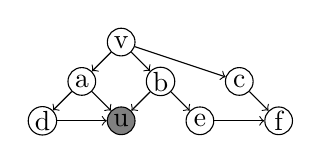
\begin{tikzpicture}[baseline=0pt]
			\begin{scope}[every node/.style={circle,draw,inner sep=0.5pt,minimum size=10pt}, treenode/.style = {circle,draw,inner sep=0.5pt,minimum size=10pt,fill=gray}]
			    \node (d) at (0,0) {d};
			    \node [treenode] (u) at (1,0) {u};
			    \node (e) at (2, 0) {e};
			    \node (f) at (3,0) {f};
			     \node (a) at (0.5, 0.5) {a};
			    \node (b) at (1.5, 0.5) {b};
			    \node (c) at (2.5, 0.5) {c};
			    \node (v) at (1, 1) {v};
			\end{scope}
			\begin{scope}[
			             every node/.style={fill=black,circle},
			              every edge/.style={draw=black}]
			    \path [->] (v) edge  (a);
			    \path [->] (v) edge  (b);
			    \path [->] (v) edge  (c);
			    \path [->] (a) edge  (d);
			    \path [->] (a) edge  (u);
			    \path [->] (b) edge  (e);
			    \path [->] (b) edge  (u);
			    \path [->] (c) edge  (f);
			    \path [->] (d) edge  (u);
			    \path [->] (e) edge  (f);
			\end{scope}
		\end{tikzpicture}
\end{filecontents*}

\begin{filecontents*}{temp3.tikz}
		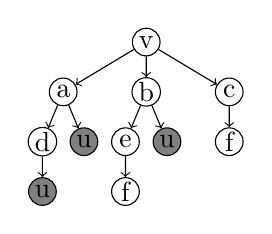
\begin{tikzpicture}[baseline=0pt,->,
		level/.style={sibling distance = 3em/#1,level distance = 1.8em}, 
		interestnode/.style = {circle,draw,fill=gray,inner sep=0.5pt,minimum size=10pt},
		treenode/.style = {circle,draw,inner sep=0.5pt,minimum size=10pt}] 
		\node [treenode] {v}
		    child{ node [treenode] {a} 
		             child{ node [treenode] {d} 
									child{ node [interestnode] {u}}			
		            }
		            child{ node [interestnode] {u}}                    
		    }
		    child{ node [treenode] {b}
		            child{ node [treenode] {e} 
									child{ node [treenode] {f}}			
		            }
		            child{ node [interestnode] {u}}
		    }
		    child{ node [treenode] {c}
		    	  child{ node [treenode] {f} 
		     }
			  }
		; 
		\end{tikzpicture}
\end{filecontents*}

\begin{filecontents*}{temp4.tikz}
  \begin{tikzpicture}[auto, 
%fill=white,
node distance=4cm,
%minimum width=3cm,
font=\small]
  
  
\node[initial,state] (A)                                    {$G_0$};
\node[ellipse (4 and 5), minimum=3cm]         (B) [above right of=A]                 {$G_1$};
\node[ellipse (3 and 2) minimum=2cm]         (C) [below right of=A]                 {$G_2$};
\node[state, minimum=1cm]         (D) [below right of=B]                 {$G_3$};
\node[state]         (E) [above right of=D]                 {$s_4$};
\node[state]         (F) [below right of=D]                 {$s_5$};

 

  \end{tikzpicture}
\end{filecontents*}


\begin{filecontents*}{temp5.tikz}
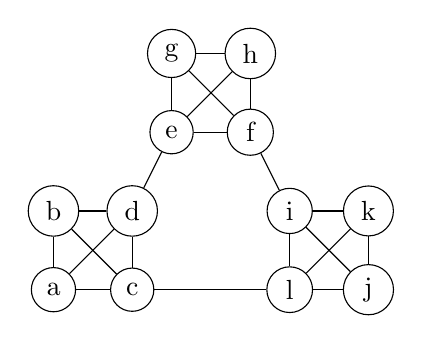
\begin{tikzpicture}
\tikzset{vertex/.style = {shape=circle,draw,minimum size=10 pt}}
\tikzset{edge/.style = {-,> = latex'}}
% vertices
\node[vertex] (a) at  (0,0) {a};
\node[vertex] (b) at  (0,1) {b};
\node[vertex] (c) at  (1,0) {c};
\node[vertex] (d) at  (1,1) {d};

\node[vertex] (i) at  (3,1) {i};
\node[vertex] (j) at  (4,0) {j};
\node[vertex] (k) at  (4,1) {k};
\node[vertex] (l) at  (3,0) {l};

\node[vertex] (e) at  (1.5,2) {e};
\node[vertex] (f) at  (2.5,2) {f};
\node[vertex] (g) at  (1.5,3) {g};
\node[vertex] (h) at  (2.5,3) {h};
%edges
\draw[edge] (b) to (a);
\draw[edge] (b) to (c);
\draw[edge] (a) to (d);
\draw[edge] (b) to (d);
\draw[edge] (c) to (a);
\draw[edge] (c) to (d);

\draw[edge] (e) to (h);
\draw[edge] (e) to (f);
\draw[edge] (e) to (g);
\draw[edge] (f) to (h);
\draw[edge] (f) to (g);
\draw[edge] (g) to (h);

\draw[edge] (i) to (l);
\draw[edge] (i) to (k);
\draw[edge] (i) to (j);
\draw[edge] (l) to (k);
\draw[edge] (l) to (j);
\draw[edge] (j) to (k);


\draw[edge] (f) to (i);
\draw[edge] (d) to (e);
\draw[edge] (c) to (l);
\end{tikzpicture}
\end{filecontents*}

\begin{filecontents*}{temp7.tikz}
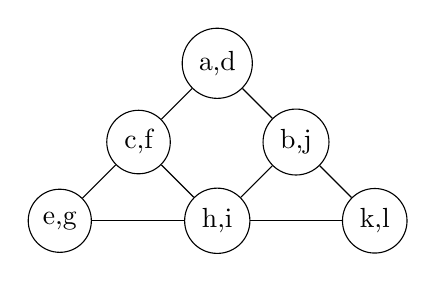
\begin{tikzpicture}
\tikzset{vertex/.style = {shape=circle,draw,minimum size=10 pt}}
\tikzset{edge/.style = {-,> = latex'}}
% vertices
\node[vertex] (a) at  (2,2) {a,d};
\node[vertex] (b) at  (1,1) {c,f};
\node[vertex] (c) at  (3,1) {b,j};
\node[vertex] (d) at  (0,0) {e,g};
\node[vertex] (e) at  (2,0) {h,i};
\node[vertex] (f) at  (4,0) {k,l};

%edges
\draw[edge] (a) to (b);
\draw[edge] (a) to (c);
\draw[edge] (b) to (d);
\draw[edge] (b) to (e);
\draw[edge] (c) to (e);
\draw[edge] (c) to (f);
\draw[edge] (d) to (e);
\draw[edge] (e) to (f);
\end{tikzpicture}
\end{filecontents*}

\begin{filecontents*}{temp6.tikz}
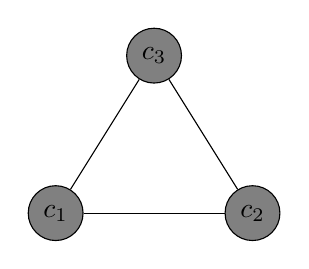
\begin{tikzpicture}
\tikzset{vertex/.style = {shape=circle,draw,minimum size=10 pt, fill=gray}}
\tikzset{edge/.style = {-,> = latex'}}
% vertices
\node[vertex] (a) at  (0,0) {$c_1$};
\node[vertex] (b) at  (2.5,0) {$c_2$};
\node[vertex] (c) at  (1.25,2) {$c_3$};
%edges
\draw[edge] (b) to (a);
\draw[edge] (b) to (c);
\draw[edge] (a) to (c);
\end{tikzpicture}
\end{filecontents*}
%%%%%%%%%%%%%%%%%%%%%%%%%%%%%%%%%%%%%%%%%%%%%%%%%%%%%%%%%%%%%%%%%%%%%%%%%%%%%%%
\begin{document}

%%%%%%%%%%%%%%%%%%%%%%%%%%%%%%%%%%%%%%%%%%%%%%%%%%%%%%%%%%%%%%%%%%%%%%%%%%%%%%%

% 制作国家图书馆封面(博士学位论文才需要)
%\makenlctitle
% 制作中文封面
\maketitle
% 制作英文封面
\makeenglishtitle


%%%%%%%%%%%%%%%%%%%%%%%%%%%%%%%%%%%%%%%%%%%%%%%%%%%%%%%%%%%%%%%%%%%%%%%%%%%%%%%
% 开始前言部分
\frontmatter


%%%%%%%%%%%%%%%%%%%%%%%%%%%%%%%%%%%%%%%%%%%%%%%%%%%%%%%%%%%%%%%%%%%%%%%%%%%%%%%
% 论文的中文摘要
\begin{abstract}
在基于图计算的数据分析应用中,如何衡量图中顶点之间的相似度是一个非常重要的课题,在很多领域有广泛的应用。
SimRank是近年来比较流行的相似性度量,相比于其它相似度指标,它能更好地反映图的拓扑结构信息。
然而它的计算代价较高,传统计算方法已经不适用于规模越来越大的图数据。
另一方面,Spark作为一种分布式计算平台能够简化用户编写分布式应用的逻辑,自问世以来迅速在学术界和产业界得到广泛的使用。
因此,基于Spark或类似平台设计高效的大规模图数据中点对SimRank相似度的分布式计算方法,有着重要的现实意义。
本文针对上述问题展开了深入的研究,取得的主要成果有:
\begin{enumerate}
 \item 针对单源点SimRank相似度计算问题,提出并实现了一种基于随机游走模型的分布式算法。
 算法通过减少随机游走的数量以及紧凑的中间数据表示来降低计算的时间和空间复杂度,通过将游走的匹配计算过程分发至整个集群
 达到高并行度,同时设计了动态规划技巧加速匹配过程。
实验结果表明,算法将随机游走的数量降低了数百倍以上,同时表现出近乎线性的可扩展性。
 
 \item 提出并实现了一种基于模块度优化的多层次分布式图划分方法,算法在划分过程中较好地保留了图中的稠密子结构,
 在考虑划分约束条件的情况下保证了顶点的均衡划分,并力求最小化各个分块之间的边割权重。
 实验结果表明,算法的划分质量可以媲美经典算法METIS,同时有较好的可扩展性。
 
 \item 针对图中全点对相似度计算问题,提出并实现了一种基于分治思路的计算方法。
 该算法通过分别计算分块内点对的相似度以及分块本身的相似度,来计算所有点对的全局相似度。
 实验结果表明,我们的方法在有效性上完全可以媲美SimRank,但计算效率得到了数倍至数十倍(3-16倍)的提高。
\end{enumerate}

% 中文关键词。关键词之间用中文全角分号隔开,末尾无标点符号。
\keywords{图数据;SimRank相似度;分布式计算;Spark}
\end{abstract}

%%%%%%%%%%%%%%%%%%%%%%%%%%%%%%%%%%%%%%%%%%%%%%%%%%%%%%%%%%%%%%%%%%%%%%%%%%%%%%%
% 论文的英文摘要
\begin{englishabstract}
In graph-based data analysis applications, how to measure similarity between vertices in a graph is a
very important research topic which has a wide range of applications in many fields.
Among all the measures, SimRank is the one with growing popularity in recent years.
Compared with others, SimRank is able to capture the topology of the  graph. 
However, computation of SimRank is costly in both time and space, making traditional computing methods
failing to handle graph data with ever-growing size.
On the other hand, as today's popular big data computing engine, Apache Spark significantly simplifies user's programming logic
with the interface it provides when developing distributed applications. 
Therefore, to design an efficient distributed algorithm to compute SimRank similarity for vertex pair in large-scale graphs
based on Spark or other systems is of great significance.

This article addresses the above problems and our main contributions are summarized as follows:
\begin{enumerate}
 \item To compute the single-source SimRank similarity, we proposed and implemented an algorithm based on the random-walk model.
 The algorithm reduces time complexity by producing less random walks, 
 reduces space complexity by compressing the representation of intermediate data,
 achieves high parallelism by distributing the matching process of random walks to the whole cluster.
 Experiments on real-world data show that the number of random walks has a decrease of two or more orders of magnitude,
 and the running time achieves near-linear scalability.
 \item We proposed a distributed multi-level  partitioning algorithm based on modularity maximization for large graphs.
 In the processing of partitioning, the local dense subgraphs are well preserved within blocks.
 Load balance of vertices is carefully maintained with respect to specific constraints, 
 and efforts are made to minimize the edge cut weights between blocks. 
 Experiments show that the algorithm achieves good partition quality comparable to METIS, and good scalability.
 \item With the help of the above graph partitioning scheme, we proposed an divide-and-conquer algorithm to 
 compute the all-pair SimRank similarity.
 The algorithm partitions the graph into blocks, obtains similarity of each node-pair within blocks, then treats each 
 block as a new vertex forming a coarsening graph to get the similarity between each block. 
 A global similarity for all vertex pairs is computed based on these two similarities.
 Experiments show that the effectiveness of our algorithm is comparable to SimRank,
 while the computing efficiency is increased by several to tens of times(3-16x).
 \end{enumerate}

% 英文关键词。关键词之间用英文半角逗号隔开,末尾无符号。
\englishkeywords{Graph Data, SimRank Similarity, Distributed Computing, Spark}
\end{englishabstract}

%%%%%%%%%%%%%%%%%%%%%%%%%%%%%%%%%%%%%%%%%%%%%%%%%%%%%%%%%%%%%%%%%%%%%%%%%%%%%%%
% 论文的前言,应放在目录之前,中英文摘要之后
%

%%%%%%%%%%%%%%%%%%%%%%%%%%%%%%%%%%%%%%%%%%%%%%%%%%%%%%%%%%%%%%%%%%%%%%%%%%%%%%%
% 生成论文目次
\tableofcontents

%%%%%%%%%%%%%%%%%%%%%%%%%%%%%%%%%%%%%%%%%%%%%%%%%%%%%%%%%%%%%%%%%%%%%%%%%%%%%%%
% 生成插图清单。如无需插图清单则可注释掉下述语句。
%\listoffigures

%%%%%%%%%%%%%%%%%%%%%%%%%%%%%%%%%%%%%%%%%%%%%%%%%%%%%%%%%%%%%%%%%%%%%%%%%%%%%%%
% 生成附表清单。如无需附表清单则可注释掉下述语句。
%\listoftables

%%%%%%%%%%%%%%%%%%%%%%%%%%%%%%%%%%%%%%%%%%%%%%%%%%%%%%%%%%%%%%%%%%%%%%%%%%%%%%%
% 开始正文部分
\mainmatter

%%%%%%%%%%%%%%%%%%%%%%%%%%%%%%%%%%%%%%%%%%%%%%%%%%%%%%%%%%%%%%%%%%%%%%%%%%%%%%%
% 学位论文的正文应以《绪论》作为第一章
\chapter{绪论}\label{chapter_introduction}
\iffalse
本章阐明本文研究工作的背景与意义,并回顾SimRank相似度计算与图划分这两个课题近年来的研究现状,然后陈述本文的主要研究成果。
本章还对Spark平台及其所提供的编程接口进行简单的介绍,旨在让读者更好地理解本文算法的设计思路与实现方案。
\fi
\section{研究背景与意义}
图(graph)作为一种能够刻画实体之间关系的抽象结构,在很多领域中有着重要的应用。
例如,电子商务中商品与用户之间的交易行为,科研著作中各类论文之间的相互参考引用,
Web中个网页之间的链接,以及社交网络中用户之间的交流传播等等行为,本质上都可以
通过基于图来建模。 从图中挖掘出深层次的信息也成了学术界以及产业界的一个重要课题。

相似性度量,即比较不同对象之间的相似度,是一个经典的问题。
在推荐系统\cite{fouss2007random}领域,人们关心哪几类商品一定程度上是相似的;
在信息检索\cite{dean1999finding}领域,人们关心如何从WWW找出相似的网页或文章,并对其聚类;
在实体解析\cite{bhattacharya2006entity}领域,人们关心如何从从复杂网络中推测出不同角色是否在真实世界代表着同一个真实实体。
可以看出,现实生活中对相似度的使用无处不在。

为了准确度量出“相似性”这一概念,学者们提出了各式各样的相似度指标。
其中,SimRank\cite{jeh2002simrank}是近年来比较流行的一种度量图中节点相似性的模型。
与传统方法不同的是,它考虑了图的拓扑结构,其基本思想与著名的网页排序算法PageRank\cite{page1999pagerank}有相似之处:
如果两个顶点的邻居顶点非常相似,那么这两个顶点也相似。
SimRank相似度可以通过随机游走模型解释,拥有坚实的理论基础,近年来在很多领域中得到了广泛的应用。

传统的SimRank计算,可以归为三类问题:1)单顶点对(single-pair)的相似度计算;
2)单源点(single-source)的相似度计算; 3)全点对(all-pair)的相似度计算。
这三个计算任务的复杂度依次增加,由计算图中某一对顶点的相似度,到图中某顶点到其它所有顶点的相似度,再到计算图中所有顶点对的相似度。
正因为SimRank试图充分利用图数据的拓扑信息,它的计算过程具有较高的时间复杂度和空间复杂度。
然而随着互联网技术的发展,人类已经跨入大数据时代。
社交网络用户呈现出爆发性地增长,电子商务正在日益普及,万维网上网络数据也不断增多,现实生活中图数据的规模越来越大。
传统的SimRank相似度计算方法已经无法适用于当下的大规模图数据。

另一方面,在大数据时代诸如MapReduce\cite{DBLP:conf/osdi/DeanG04}、Spark\cite{DBLP:conf/hotcloud/ZahariaCFSS10}等通用式分布式计算平台日益流行。
这些计算平台充分发挥了分布式集群的威力,谋求计算能力在横向上扩展(Scale Out)而不是在纵向上提高(Scale Up),使得原来难以完成的计算分析任务成为可能。
基于这些平台,用户可以使用其提供的编程接口专注于自己的计算任务,快速部署出自己的解决方案,
而无需关心分布式平台底层的复杂网络通信、资源分配、资源调度等问题。

目前现有的分布式计算方法主要是按照Map-Reduce编程范式的直接计算,或是基于矩阵计算,而对于顶点数超过百万的大图,其邻接矩阵的元素规模超过万亿。
面对如此庞大的输入规模,传统基于矩阵计算的方法根本无法满足需求。
因此,面向日益增长的大规模图数据处理的需求,设计新的分布式SimRank相似度计算方法就显得非常必要。


\section{研究现状}
\subsection{SimRank计算研究现状}
如何衡量实体之间的相似性一直是各领域研究的热点,许多研究在特定应用领域提出了各式各样的相似度度量标准。
例如Jaccard similarity \cite{jaccard1901etude}, cosine similarity \cite{baeza1999modern}, Dice similarity\cite{dice1945measures}等等。
反映在图数据中,这些相似度的核心思想都是“如果两个顶点拥有越多共同的邻居顶点,那么它们越相似”。
显然,这些度量没能够反映出图的拓扑信息。最简单的反例是,对于没有共同邻点的点对,上述度量会简单认为它们没有丝毫的相似度。
\begin{figure}[h]
  \centering
  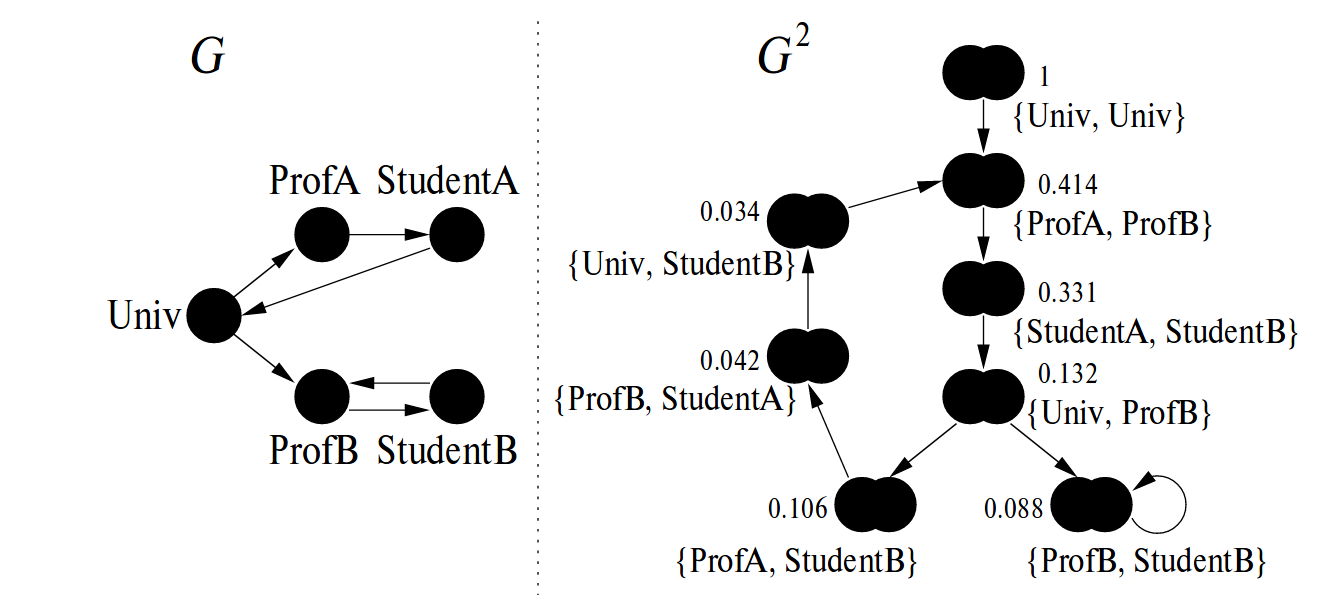
\includegraphics[width= 0.75\textwidth]{figure/simrank.png}\\
  \caption{一个简单图的SimRank计算结果。左边为原图,右边为原图的平方图(product graph)以及点对之间的相似度数值}
  \label{fig:simrank_example}
\end{figure}

SimRank\cite{jeh2002simrank}最早被用于衡量图中顶点所处于的结构上下文之间的相似性。
SimRank的核心理念借鉴了PageRank\cite{page1999pagerank},即“如果两个对象都与相似的对象相关,那么它们越相似”。
更具体地说,如果实体$a$和$c$有关联,实体$b$和$d$有关联,而且$c$和$d$有较高相似性,那么$a$和$b$也相似。
它的有效性可以由图论中的随机游走模型直观地解释,又因为它基于图这种可以刻画各种关系的离散结构,
因此自提出以来,SimRank在很多不同的领域都有广泛的应用。
图\ref{fig:simrank_example}展示了一个学校两位教授ProfA和ProfB,他们的学生StudentA和StudentB的个人主页,以学校Univ的主页之间的引用关系。
应用SimRank解释如下:因为ProfA和ProfB的主页都引用了Univ的主页,可以认为他们具有某种程度上的相似性;又因为他们分别引用了StudentA和StudentB的主页,因此StudentA和StudentB
之间也有了相似性。图中右半部分是基于SimRank计算出的具体相似度。

SimRank的计算过程具有较高的时间和空间复杂度。
为了能够处理规模日益增长的图数据,近年来学术界提出了很多致力于提高SimRank计算效率的方法。
典型的加速技巧包括快速矩阵乘法\cite{yu2012space},减少生成随机游走数量的蒙特卡罗抽样方法\cite{kusumoto2014scalable},
通过线性化的代数方法消除计算递归性\cite{DBLP:journals/corr/MaeharaKK14},
基于分布式计算的算法\cite{cao2012delta}等等。
这些算法面向特定场景,或多或少地提高了计算效率。
然而这些方法中单计算节点算法在处理超大规模的图数据时无能为力,而已有的少数分布式算法在计算效率与可扩展性上仍然存在着较大的提升空间。
另一方面,一些致力于改进SimRank有效性的新相似性度量也相继被提出,典型的有coSimRank\cite{DBLP:conf/acl/RotheS14},
SimRank++\cite{DBLP:journals/pvldb/AntonellisGC08},
P-Rank\cite{DBLP:conf/cikm/ZhaoHS09}等等。
此外,一些工作研究如何将SimRank拓展到特殊的图数据上,例如如何在不确定图\cite{DBLP:conf/icde/ZhuZL16}(uncertain graph)上衡量点对的相似性。

\subsection{图划分研究现状}
图划分是一个经典的NP完全问题。典型图划分问题的主要优化目标包括:划分结果力求均衡,即每个分块中的顶点数目大致相等;
最小化横跨不同分块的边的数量。图\ref{fig:partition}展示了对同一个图的两种划分结果。
从图中可以很直观地区分出划分质量的好坏。

\begin{figure*}[h]
\centering
\begin{subfigure}[b]{0.45\textwidth}
	\center	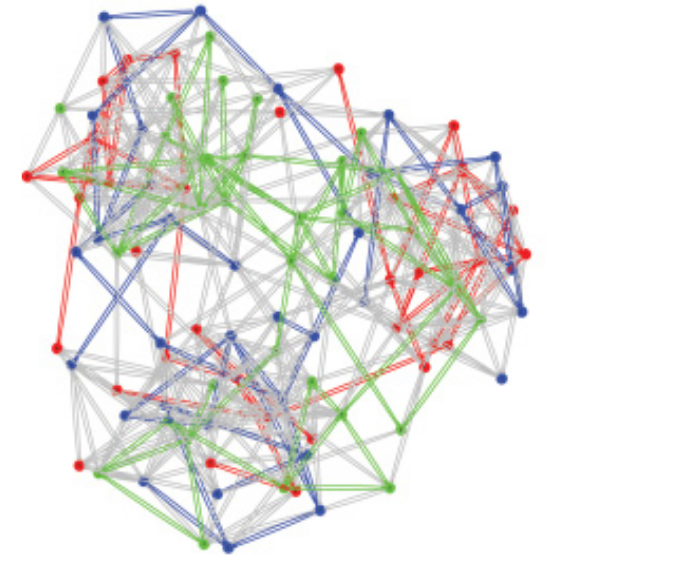
\includegraphics[width=1\textwidth]{figure/partition_a.png}
	\label{fig:p_1}
	\caption{随机划分}
\end{subfigure}
\begin{subfigure}[b]{0.45\textwidth}
	\centering
	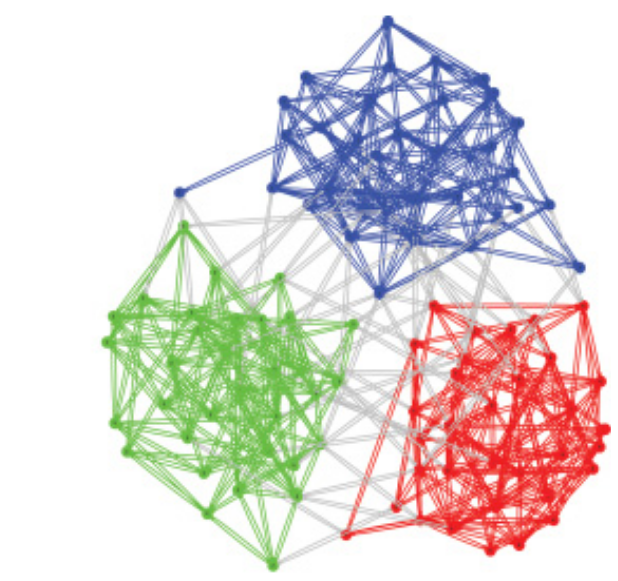
\includegraphics[width=1\textwidth]{figure/partition_b.png}
	\caption{高质量划分}
	\label{fig:p_2}
\end{subfigure}
\caption{对同一个图的两个划分。 左图是随机划分结果,其边割集较大;右图划分质量高,其边割集较小,并且图中的稠密子图得到了保留}
\label{fig:partition}
\end{figure*}

目前国内外对图划分问题进行了广泛而深入的研究。
传统的划分方法可以分为以下几种:谱方法、启发式算法、智能优化算法、多层次划分算法等。
谱方法\cite{DBLP:journals/siamsc/HendricksonL95}最早应用于图的二划分,
其基本思想是利用图的拉普拉斯矩阵的第二大特征值和特征向量来实现图的划分,它的计算开销非常大;
启发式方法基于图中局部的启发信息对问题进行求解,典型的代表有KL\cite{kernighan1970efficient}算法和FM\cite{fiduccia1988linear}算法,它们能处理的图规模非常有限;
智能方法典型的有遗传算法\cite{bui1996genetic}、模拟退火\cite{johnson1989optimization}等,它们通过对自然界的一些行为进行仿生模拟对划分问题进行优化,
其划分结果有一定概率陷入局部最优解;
多层次图划分的算法的典型代表是METIS\cite{Karypis95metis}。它通过塌缩-初始化分-恢复的迭代过程首先将图的规模降低到可以接受的范围,
再基于一定的优化思想给出该小规模图的划分,最后将划分投影成原始图上的划分。多层次方法可以处理更大规模的图数据,
其思想受到了很多其它方法的借鉴。

但总的来说,相比于如今大数据时代庞大的数据规模,上述这些方法能处理的图数据的规模仍然比较小。
随着网络中用户规模的不断扩大,一些网络图动辄有数十亿个顶点和上万亿条边,
普通的计算机由于内存的限制根本无法处理,这给常见的图计算任务带来巨大的挑战。
在此背景下,设计开发高效的分布式图数据划分方法是未来的主要方向。

\section{技术背景}
\iffalse
对分布式算法而言,其实际的运行效率与底层计算平台密不可分,甚至计算平台的一些机制会成为算法设计过程中的主要着眼点。
本文所有的算法都基于分布式计算平台Spark以及构建在Spark之上的图计算平台GraphX实现,本节粗略介绍它们的背景知识。
\fi
\subsection{Spark背景介绍}
Aparch Spark\cite{DBLP:conf/hotcloud/ZahariaCFSS10}是由UC Berkeley AMP Lab开发的通用分布式计算平台,
目前它已经成为Apache Software Foundation下大数据开源项目中最流行的项目之一。
Spark遵循类似于MapReduce的编程范式,它引入了RDD(弹性分布式数据集)的概念,可以表达更丰富的语义。
在执行效率上,它改进了Hadoop\cite{DBLP:conf/osdi/DeanG04}批处理框架在迭代计算、交互式处理方面的不足,
允许应用在内存中保存工作集以便高效地重复利用,应用程序的性能得到数十倍甚至百倍的提升;
在用户易用性上,Spark提供了更灵活的编程API,方便用户对数据进行更灵活的操控。
在通用性上,Spark针对不同的开发需求提供了高阶的库,包括SQL查询,流式计算,机器学习以及图计算等等。
开发者可以根据自己的需要,单独或组合使用这些库来处理复杂的数据分析任务。
\begin{figure}[h]
  \centering
  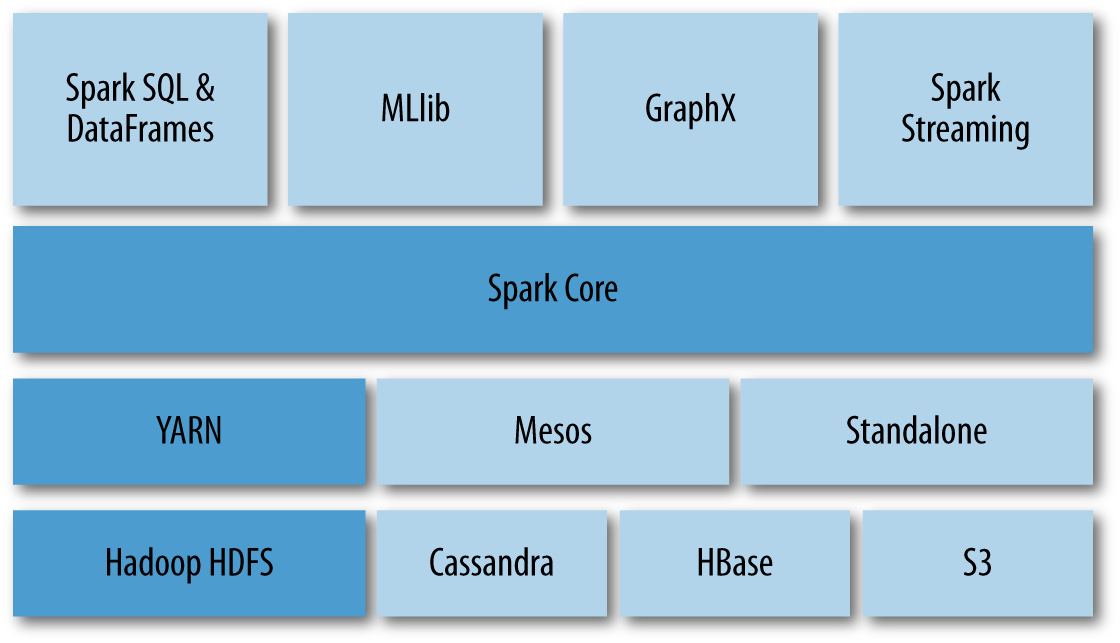
\includegraphics[width= 0.8\textwidth]{figure/spark_ssstack.png}\\
  \caption{Spark生态圈}
  \label{fig:spark_stack}
\end{figure}

目前,Spark已经成长为包含Spark SQL,Spark Streaming, MLlib, GraphX等多个子项目的完善的生态系统。
使用Spark,用户只需调用编程接口来实现自己的数据计算任务,而无需关心数据的具体分布、并行调度策略、集群节点之间的数据传送与错误恢复等复杂的底层细节。
凭借其高效、用户友好、通用的优点,Spark在学术界和工业界得到了广泛的实际应用。


如图\ref{fig:spark_components}所示,一个典型的Spark集群通常包括以下几个核心组件:
\begin{enumerate}
 \item Driver Program。 每一个Spark应用程序都包含一个驱动程序,它执行用户的main函数,并负责在集群调度所有的并行化操作。
当应用程序刚从客户端提交上来的时候,驱动程序连接到负责整个集群资源分配分配的Cluster Manager,并向其请求集群上可用的Executor。 
\item Cluster Manager。 它是负责处理集群中各种资源申请要求的一个服务。Spark支持Mesos,YARN等模式。
\item Executor。 它运行在集群中每一个Worker Node上,负责本节点上所有的计算任务。Executor通常以多线程方式并行计算具体的计算任务。

\end{enumerate}

\begin{figure}[h]
  \centering
  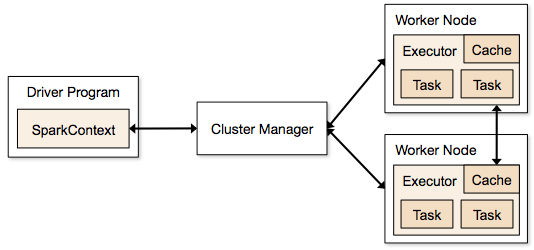
\includegraphics[width= 0.7\textwidth]{figure/spark_components.png}\\
  \caption{Spark系统架构}
  \label{fig:spark_components}
\end{figure}
%\subsection{Spark数据模型}
Spark采用了一种被称为弹性分布式数据集\cite{DBLP:conf/nsdi/ZahariaCDDMMFSS12}(RDDs, Resilient Distributed Datasets)的分布式数据抽象。
RDD是一种只读不可变的对象,并且天然就是分布式的,数据分布在整个集群中,更具体地说是执行上下文即Executor所在的JVM中。
但这一点对用户来说是透明的,对用户而言,操作RDD和操作list,map等经典的数据结构没有太大的不同。
RDD中的数据元素是有绑定类型的,通常它们存放在内存中,但Spark也提供了其它的持久化选项。
RDD通过记录创建RDD的一系列操作(lineage),也就是记录RDD如何从原始数据演变成当前状态来实现容错机制。

Spark提供了两种类型的操作:转换(transform)和动作(action)。 
转换操作在已有的RDD上执行数据变换,返回一个新的RDD,典型的转换包括filter,map,union,flatMap等。
动作则在RDD上触发实质的计算,通常是为了返回结果给调用方或者将计算结果写入到稳定的存储介质(比如磁盘)中,典型的动作包括count,saveAsTextFile,collect等。
一般可以根据返回类型来判断一个操作是转换还是动作。
转换最重要的特点是它是一种惰性操作(lazy operation),真正的变换逻辑只有在调用动作的时候才会真正发生。
当动作被触发时,Spark检查RDD的lineage,并使用这些信息构建一个操作流图(graph of operations),然后执行这些计算流程得到最终的RDD。

\iffalse
\begin{figure}[htbp]
  \centering
  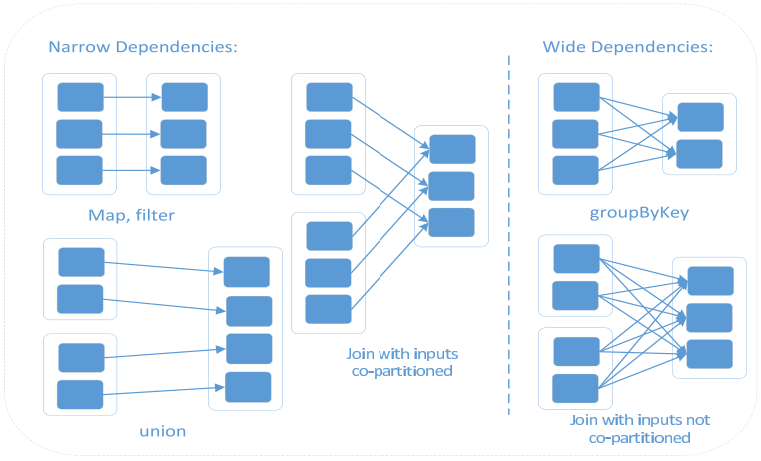
\includegraphics[width= 0.7\textwidth]{figure/rdd_dependency.png}\\
  \caption{Spark系统架构}
  \label{fig:rdd_dependency}
\end{figure}
%\subsection{Spark常用编程接口}

Spark提供的编程接口,主要包括两类:转化和动作。
其中,典型的转化包括以下几类: 
\begin{enumerate}
 \item {\asciifamily map}一个RDD可以通过map将RDD中的每一个元素通过用户指定的函数转化为另一种类型的元素,
 也就是将原来的RDD转变为指定类型的RDD。map函数接受的参数是一个函数算子。
 \item {\asciifamily mapValues}与map类似,mapValues用于类型为(key, value)的PairRDD。不同的是mapValues不改变元素的key而只改变元素的value,
 因此新的RDD会保留原RDD的partitioner。
 \item {\asciifamily mapPartitions}与map类似,它的第一个参数是一个函数,但mapPartitions是对原RDD的每一个partition而不是每一个element实施这个函数;它的第二个参数是一个Boolen类型,当原RDD的元素类型为(key, value)键值对,并且mapPartitions操作不会改变元素的key时,
 将第二个参数设为true告诉Spark不要改变RDD的partitioner。
\item {\asciifamily filter}一个RDD可以通过filter对RDD中的所有元素按照一定条件进行过滤,过滤后的元素组成一个新的RDD。因此,filter函数接受的参数是一个返回类型为Boolean的函数,这个函数指明一个元素能不能通过筛选。
\item {\asciifamily join}两个元素类型为(key, value)的PairRDD可以通过join操作将双方key相同的元素合并,返回一个新的RDD。
\item {\asciifamily union}两个RDD可以通过union操作合并为一个RDD。
\item {\asciifamily reduceByKey}一个PairRDD调用这个操作可以将原RDD中key相同的若干元素规约为一个元素,返回一个新的RDD。它的第一个参数是一个函数,这个函数相当于元素之间的运算符;第二个可选的参数可以指定新RDD的partition个数。类似于Hadoop中的combiner,spark在shuffle之前会首先对每个计算节点本地的元素先进行合并,从而减小shuffle的开销。
\end{enumerate}
典型的动作包括以下几类:
\begin{enumerate}
 \item {\asciifamily reduce} 它的参数是一个满足交换律、结合律的二元运算符,原RDD的所有元素经过这个运算符计算,返回一个最终值。
 \item {\asciifamily collect} 它将RDD中所有元素从集群上以一个数组的形式返回到Driver Program。collect是一个开销非常大的操作,只适合在小数据集上调用。
\end{enumerate}
还有一种比较特殊的广播操作。通常来说,当集群中的某个节点计算过程中发现需要使用用户自定义的变量时,会向driver program请求将该变量传送到该节点,每一个节点单独地对本地的变量副本进行计算,计算过程中对该副本做出的改动并不会反映到driver program。Spark提供了一种广播变量(broadcast variable), 
它允许开发者主动地将可能在在节点用到的变量广播到集群中的每个节点上,而不用在程序执行过程中当特定节点发现要使用这个变量再从driver program发送到这个节点上。Spark在传送广播变量时使用了一些高效的算法,减少了广播过程中的通信开销。文献[15]表明,在进行迭代计算时,广播变量能极大地提高整体性能。
\fi

\subsection{GraphX背景介绍}
GraphX\cite{DBLP:conf/osdi/GonzalezXDCFS14}是Spark生态圈中的一个核心组件, 主要用于图并行计算。
它为图计算和图挖掘任务提供了简洁易用的接口,极大的简化了用户对图计算任务的编程。
GraphX通过引入一个新的图抽象来拓展Spark中的RDD: Resilient Distributed Property Graph,一种点和边都附带属性的有向多重图。
这里的属性(property)指的是用户自己定义的描述边或顶点某些性质的对象。
一个典型的属性图中包含了描述节点信息的VertexRDD和描述边信息的EdgeRDD。
图\ref{fig:property_graph}描述了一个表示反映科研工作者人事关系的图,以及改图在GraphX对应的属性图的底层存储。
\begin{figure}[h]
  \centering
  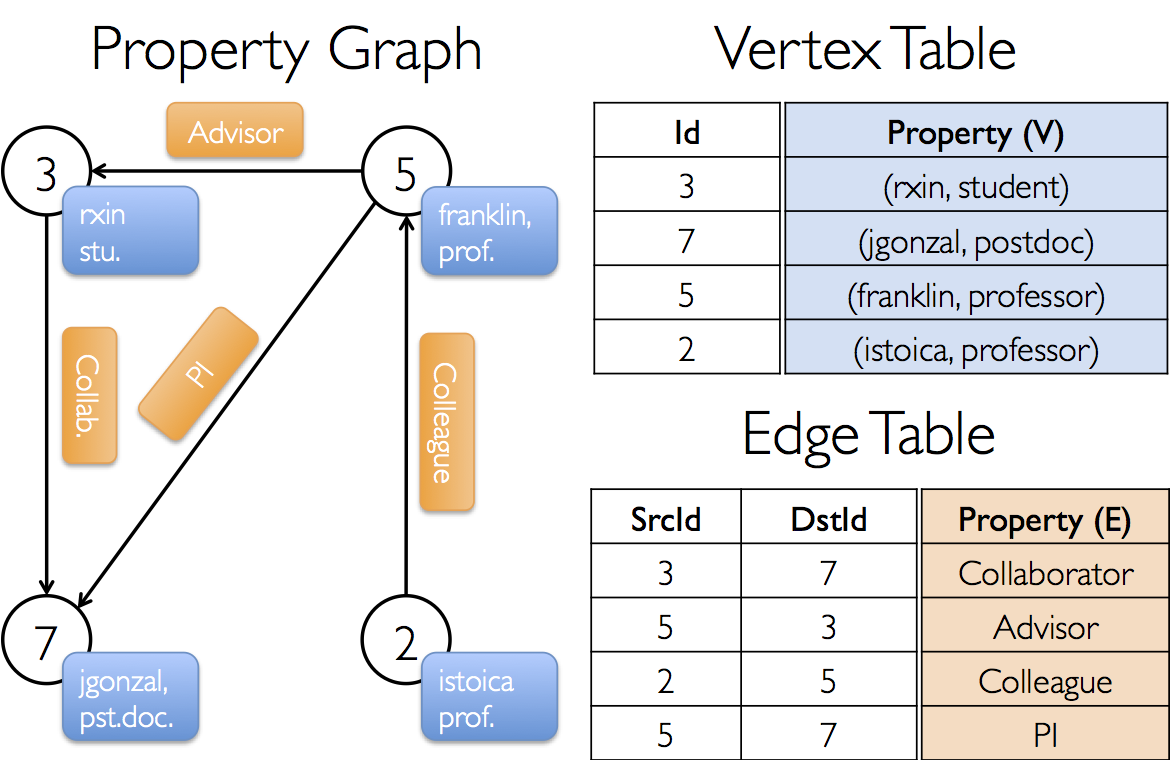
\includegraphics[width= 0.7\textwidth]{figure/property_graph.png}\\
  \caption{一个简单的属性图。左图为图的拓扑信息及其关联的属性;右图为该属性图底层存储的RDD}
  \label{fig:property_graph}
\end{figure}

和RDD一样,属性图是不可变的、分布式的、容错的。
对图的内容或者结构的改变需要生成一个新的图来实现。
对属性图的所有操作,最终都会转换成其关联的VertexRDD和的EdgeRDD上的相关操作。
这样一个图计算任务在最终都等价于一系列RDD的转换过程。
其中,原始图的不受影响的部分都可以在新图中重用,用来减少这种固定功能的数据结构的成本,这对用户是透明的。
除了属性图的顶点和边视图,GraphX也包含了一个三元组视图。
三元视图逻辑上将顶点和边的属性保存为一个RDD[EdgeTriplet[VD, ED]],它包含EdgeTriplet类的实例,具体细节如图\ref{fig:triplet}所示。

%\subsection{GraphX编程范式}
\begin{figure}[h]
  \centering
  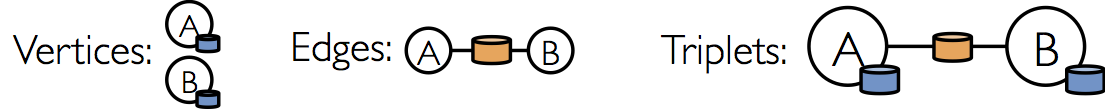
\includegraphics[width= 0.7\textwidth]{figure/triplet.png}\\
  \caption{GraphX的提供的三种视图对比:顶点,边,三元组}
  \label{fig:triplet}
\end{figure}

GraphX通过类Graph来暴露核心的编程接口。
图\ref{fig:Graph}展示了Graph的定义及其能提供的核心操作(为了展示效果内容有所筛选),这些方法在本文算法的实现中都有大量运用。
\begin{figure}[h]
  \centering
\begin{lstlisting}
/** Summary of the functionality in the property graph */
class Graph[VD, ED] {
  // Information about the Graph 
  val numEdges: Long
  val numVertices: Long
  val degrees: VertexRDD[Int]
  // Views of the graph as collections 
  val vertices: VertexRDD[VD]
  val edges: EdgeRDD[ED]
  val triplets: RDD[EdgeTriplet[VD, ED]]
  // Transform vertex and edge attributes 
  def mapVertices[VD2](map: (VertexID, VD) => VD2): Graph[VD2, ED]
  def mapEdges[ED2](map: (PartitionID, Iterator[Edge[ED]]) => Iterator[ED2]): Graph[VD, ED2]
  def mapTriplets[ED2](map: EdgeTriplet[VD, ED] => ED2): Graph[VD, ED2]
  // Aggregate information about adjacent triplets 
  def collectNeighborIds(edgeDirection: EdgeDirection): VertexRDD[Array[VertexID]]
  def collectNeighbors(edgeDirection: EdgeDirection): VertexRDD[Array[(VertexID, VD)]]
  // Basic graph algorithms 
  def pageRank(tol: Double, resetProb: Double = 0.15): Graph[Double, Double]
  ...
}

\end{lstlisting}
  \caption{类Graph包含的部分属性与方法}
   \label{fig:Graph}
\end{figure}
\section{本文主要研究工作}
分析已有的计算方法我们发现,传统的单机SimRank计算方法对于大规模的图数据无能无力,
现有的分布式算法基本采用了直接计算或矩阵计算的思路。
而对于一个顶点数目为百万级别的图,其矩阵的元素基本在万亿级别以上。
面对如此大的计算规模,即便分布式矩阵处理也无能为力。
在此背景下,本文针对大规模图数据中点对SimRank相似度的分布式并行计算问题,进行了深入的研究。
本文的主要研究成果具体如下:
\begin{enumerate}
\item 针对单源点SimRank相似度的计算,提出并实现了一种基于随机游走模型的分布式计算方法。
整个算法包含三个步骤:首先生成随机游走,再对游走进行匹配计算其对应概率,
最后汇总得出相似度。
针对计算本身的高时间复和空间复杂度,本文设计了一系列方法来提高计算效率,包括减少随机游走的数量,使用更紧凑的数据结构来压缩中间数据,以及通过动态规划
的技巧加速随机游走的匹配计算。
本文还对算法的复杂度给出了详尽的分析。
在真实数据集上的实验结果表明,算法对随机游走的数量降低了数百倍以上,
同时表现出近乎线性的可扩展性。

\item 针对大规模图数据,提出一种分布式图划分方法。
该算法能够在保留图中稠密子结构的同时,对图中顶点进行尽量均匀的划分,同时最小化划分之间边的数量(或权重)。
实验结果表明该划分方法在划分质量上可以媲美经典的METIS,同时有较好的可扩展性。

\item 基于上述的图划分方法,进而提出一种计算所有顶点之间相似度的分布式计算方法。
该方法使用分而治之的思想,将所有点对的计算问题划分为若干个子问题,最后再基于子问题的解聚合出原始问题的解。
具体地说,算法首先对图进行划分,然后对每个分块内的顶点对计算局部相似度,然后将各个分块抽象为新的顶点形成一个粗化的加权图并计算各个分块之间的相似度,
最后通过局部相似度和分块相似度共同计算出所有点对的全局相似度。
实验结果表明,我们的方法在有效性上完全可以媲美SimRank,但计算效率得到了数倍至数十倍(3-16倍)的提高。

\item 对上述计算方法,我们分别在流行的通用计算平台Spark上给出其分布式实现,并使用真实的数据集
在验证算法的精度、效率,以及可扩展性。

\end{enumerate}
\section{论文结构}
本文一共5个章节,每个章节的安排如下:

第一章:绪论。 分别论述了研究背景和意义、研究现状以及现阶段研究尚存在的问题、技术背景、本文的主要研究工作和文章总的框架结构。

第二章:分布式单源点SimRank相似度算法。 
该章首先对SimRank构建基于随机游走的模型,然后提出算法的框架以及算法中的若干设计思路,接着基于Spark平台实现算法,
最后用实验验证算法各方面的性能。

第三章:基于模块度优化的分布式图划分方法。 该章首先分析了典型的图划分过程的目标和难点,然后对比社区发现与图划分这两个任务的异同,
提出了使用基于模块度的社区发现算法来进行图划分任务。 接着提出算法的主要流程,包括塌缩、初始化分、恢复三个步骤。
我们基于Spark平台给出算法的总体实现,最后通过实验验证算法各方面的性能。

第四章:分布式全点对相似度算法。 该章首先将全点对的相似度计算划分为两个层面的相似度:分块内相似度和分块间相似度。
然后分别给出了这两个相似度的具体计算方法。接着提出了基于上述两个相似度来计算全局相似度的方法。
我们基于Spark平台给出算法的总体实现,最后通过实验验证算法各方面的性能。

第五章:总结与展望。总结本文阐述的算法,并对下一步工作做出展望。


%%%%%%%%%%%%%%%%%%%%%%%%%%%%%%%%%%%%%%%%%%%%%%%%%%%%%%%%%%%%%%%%%%%%%%%%%%%%%%%
\chapter{分布式单源点相似度算法}\label{chapter_sssSimRank}
\iffalse
本章关注单源点SimRank相似度计算问题:给定一个查询顶点$u$,计算$u$与图中所有其它顶点$v$之间的相似度$s(u,v)$。
本章首先对SimRank基于随机游走建模,并从该模型出发,优化每个步骤的时间复杂度、空间复杂度、可并行度,进而提出一个分布式计算方法。
\fi
\section{概述}
SimRank是一个基于结构上下文的相似度模型,它的核心思想是:如果两个顶点的邻居顶点非常相似,那么这两个顶点也相似。
单源点SimRank相似度计算问题,相比于的单点对和全点对的相似度计算,单源点问题的计算复杂度正好居于它们二者之间,
它在实际问题中运用的最多。
这是因为对于大规模图数据而言,尤其是对于类似社交网络这样的拓扑结构无时无刻都在变化的图来说,频繁计算所有点对的相似度开销过于巨大。
另一方面,每次只计算单点对相似度又显得粒度过细。
单源点问题的另外一种常见变种是相似度的top\string-k查询问题,即如何选取与$u$最相似的$k$个其它顶点。
诸如此类的查询在各个领域有大量的实际应用。

为了方便描述,首先给出一些通用的符号定义。本文使用关系$(V, E)$表示一个有向图,其中 $V$是图的顶点集合,
$E \subseteq V \times V$ 是图中边的集合。
$n$ 和 $m$分别是图中顶点的个数、边的个数。顶点$u$ 称作顶点 $v$的入邻点(或出邻点),当且仅当$(u, v)$(或$(v,u)$) 是 $G$中的一条边。
顶点$u$ 的所有入邻点用符号 $I(u)=\{v: (v, u) \in E\}$ 表示,所有出邻点用符号 $O(u)=\{v: (u, v) \in E\}$表示。
图中所有顶点的平均入度(同样也是出度)用符号$d$表示。
顶点$u, v$间的SimRank相似度由$s(u, v)$表示,相应地,所有点对的相似度可以写作 $n\times n$的相似度矩阵$S$,并且有$s(u, v)=s_{uv}$。
顶点$u, v$间的相似值用数学公式如下表达:
\begin{equation}
s(u, v) = \left\{
        \begin{array}{ll}
	1 & \quad u = v  \\
	\displaystyle\frac{c}{|I(u)||I(v)|}\displaystyle\sum_{u^\prime \in I(u), v^\prime \in I(v)} s(u^\prime, v^\prime) & \quad u \ne v
        \end{array}
    \right.
	\label{eq:one}
\end{equation}
其中,$0 < c < 1$是衰减系数,用以提高邻近处结构对最终相似性的贡献权重,同时降低偏远处结构的贡献权重。
文献\cite{jeh2002simrank}证明了上面的式子总是存在唯一的解,并且基于SimRank的定义,提出了一种基于矩阵乘法的迭代算法。
设 $S^k$是相似度矩阵$S$在第$k$轮迭代中的计算结果,$S^0$为矩阵初始值,并且如果有$u = v$那么有$S^0_{uv} = 1$,否则$S^0_{uv} = 0$。
则矩阵$S^{k+1}$的计算方式如下:
\begin{equation}
S^{k+1}_{uv} = \left\{
        \begin{array}{ll}
	1 &\hspace{-0.5em}  \! u = v  \\
	\displaystyle\frac{c}{|I(u)||I(v)|}\displaystyle\sum_{u^\prime \in I(u), v^\prime \in I(v)} S^{k+1}_{u^\prime v^\prime}  & \hspace{-0.5em} u \ne v
        \end{array}
    \right.
	\label{eq:two}
\end{equation}
文献\cite{jeh2002simrank}已经证明,$\lim_{k\to\infty}S^k_{uv} = s(u,v)$。可以看出,该算法的时间复杂度为$O(n^2)$,空间复杂度为$O(kn^2d^2)$。

\section{相关工作}
目前学术界对单源点SimRank点对的相似度计算问题的研究,可以概括为如下几类:

\textbf{单节点串行算法。 }Jeh和Widom\cite{jeh2002simrank}首先对SimRank完成了基于随机游走的建模:图中顶点$u$,$v$的相似性,
可以解释为以顶点$u$和顶点$v$分别为初始点同步移动的随机游走第一次在某个顶点相遇的概率的期望值。
文献\cite{fogaras2005scaling}给出了一个基于随机游走的算法,该算法首先为$N$个随机游走建立一个大小为$O(nN)$的索引,然后基于索引查询点对的相似性。
该算法可以给出理论上的结果误差分析,然而建立索引过程需要大量预处理时间。
SLING\cite{DBLP:conf/sigmod/TianX16}也采用了类似的思路,它构建了专门用于加速相似度计算的索引结构,然而索引的代价非常高昂,
其空间复杂度超过图本身的空间复杂度一个量级。
文献\cite{kusumoto2014scalable}提出一种方法对随机游走使用采样技巧计算点对的相似性,该方法在允许一定程度精度损失的情况下提高了计算效率。
文献\cite{lee2012top}研究了图中top-$k$个最相似点对的查询问题,该方法把点对相似度查询转变为顶点规模为$n^2$的乘积图$G^2$上的查询问题,
由于$k$往往是一个非常小的值,该问题是单源点相似度计算的一个子集。

\textbf{分布式并行算法。 }
文献\cite{DBLP:journals/pvldb/LiFLCCL15}提出了一种并行化蒙特卡罗采样的分布式计算方法,该方法打破了计算点对相似性之间的递归依赖关系:首先线下计算一个不变矩阵$D$,然后线上根据$D$使用
蒙特卡罗方法快速给出查询。该算法的优点是它是一种通用的方法,可以同时应对单点对、单源点、全点对的相似度计算问题。
然而,$D$的计算被当做一个解线性方程组的过程,这在分布式环境下非常低效,因此虽然算法线上查询的效率很高,
但线下预处理的时间开销非常巨大。它可以处理十亿级别的大规模图,但是在一个拥有10个计算节点且总内存高达3.77TB的集群中,需要大约110小时的预处理时间。
\section{算法基本框架}
%本节首先对SimRank基于随机游走建模,并从该模型出发,优化每个步骤的时间复杂度、空间复杂度、可并行度,进而提出一个分布式计算方法。
\subsection{基于随机游走的SimRank建模}
SimRank相似度可以基于随机游走进行建模。
序列$W=v_0v_1v_2\dots v_l$ 如果对任意$0 \leq i \leq l-1$都满足 $(v_i, v_{i+1})$ 是 $G$ 中的边,
则称其为 $G$中的一个游走。如果$W$还满足以下的Markov条件,即对所有的$i \geq1$ ,   $v_0, v_1, \dots, v_i \in V$,有:
\begin{eqnarray}
\label{eq:three}
  Pr(X_i = v_i|X_{0} = v_{0},\dots, X_{i-1}  = v_{i-1}) \nonumber \\  
 =  Pr(X_i = v_i|X_{i-1} = v_{i-1})
\end{eqnarray}
则称其为随机游走。
其中,$X_i$ 表示在第$i$步游走正好到达的顶点。
对任意$ u,v \in V$, $Pr(X_i=v|X_{i-1}=u)$表示在第$i-1$步到达顶点$u$的随机游走将在第$i$步到达顶点$v$的条件概率。
对于SimRank问题,每一条随机游走从某个顶点出发,然后顺着图$G$中的逆边,每一个步骤随机走向该顶点的某一个入邻点,那么其转移概率为:
\begin{equation}
Pr(X_i=v_i|X_{i-1}=v_{i-1}) = \left\{
        \begin{array}{ll}
	\frac{1}{|I(v_{i-1})|} & \quad (v_i, v_{i-1}) \in E \\
	0  &\quad otherwise
        \end{array}
    \right.
	\label{eq:four}
\end{equation}
相应地,一条随机游走的概率,定义为:
 \begin{equation}
Pr(W) = \prod_{i=1}^{l}Pr(X_i=v_i|X_{i-1}=v_{i-1})
	\label{eq:seven}
\end{equation}
现在假设图$G$中有两条随机游走分别从顶点$u$和顶点$v$同时出发,顺着图中的逆边以相同速度移动,
如果这两条随机游走在同一个顶点$x$相遇并且为它们的初次相遇,我们就把这两条终止在顶点$x$的游走称作“匹配游走”。
每一对匹配游走的长度就等于随机游走的步骤数。我们基于此定义相遇概率:
 \begin{equation}
Pr\big((W_u, W_v)\big) = Pr(W_u)Pr(W_v)
	\label{eq:five}
\end{equation}
文献\cite{jeh2002simrank}表明,节点$u,v$之间的相似度$s(u,v)$等于服从上面概率分布的若干匹配游走的期望:
 \begin{equation}
s(u,v) = \sum\limits_{W_u, W_v} c^lPr\big((W_u, W_v)\big)
	\label{eq:six}
\end{equation}
其中, ($W_u$, $W_v$) 是一对任意的匹配游走,$l$是游走的长度,$c$是前文定义的衰减系数。
显然考虑的游走的长度越长,最后计算得到的相似性越精确。
然而想要枚举出任意长度(包括正无穷)的随机游走显然是不可行的。在现实应用中,我们考虑长度为$k < 10$的游走得到的数值可以满足一般应用。

文献\cite{li2010fast}提出了一个计算单点对SimRank相似度的算法spSimRank。算法的核心思想是两个随机冲浪者分别从顶点$u,v$出发,
每一步顺着所在顶点的入边移动,并且每经过一个顶点$t$,原来的随机游走会产生$|I(t)|$ 个新的游走。这样的话经过$k$移动之后,总共会产生
$O(d^k)$ 个不同的游走,每条随机游走的长度不超过$k$。
这些游走被保存在叫做Path-Tree的数据结构中。算法然后对两个path-Tree中的所有随机游走
进行匹配,找出其中的匹配游走,计算相遇概率并得到最终的相似度。
与基于矩阵迭代计算的计算方式相比,该算法“求近舍远”,只考虑对相似度贡献最大的那些游走,而不需要考虑图中所有的节点。
如果我们从这个算法出发,可以轻易得出一个通过暴力枚举求单源点SimRank相似度的方法,如算法\ref{algo:nssSimRank}所示。

\begin{algorithm}[h]
\captionof{algorithm}{Naive Single-source SimRank:nssSimRank}
\label{algo:nssSimRank}
\begin{algorithmic}[1]
\Procedure{SingleSourceSimRank}{$G, u, k$}
	\For{$ l =1$ to $k$}
		\State $W_u[l] \gets $ all walks of length $l$ starting from $u$;
	\EndFor
	\For {$v \in V(G)$}
		\State $s(u,v)\gets$  \Call{spSimRank}{$G, W_u[], v, k$};
	\EndFor
	\State \textbf{return} $s(u, *)$.
\EndProcedure
\Procedure{spSimRank}{$G, W_u[], v, k$}
\State $s(u, v) \gets 0$;
\For{$ l =1$ to $k$}
	%\State $W_u[l] \gets $ all walks of length $l$ starting from $u$;
	\State $W_v[l] \gets $ all walks of length $l$ starting from $v$;
	\State $s_l(u, v) \gets 0$;
	\For{ $w_u$ in $W_u[l]$}
		\For{ $w_v$ in $W_v[l]$}
		\If {$w_v$ and $w_u$ first meet at index $l$}
			\State add  $score(w_u, w_v)$ to  $s_l(u, v)$;
			\State {\Comment{According to Eq. (\ref{eq:six})}}
		\EndIf
		\EndFor
	\EndFor
	\State add $s_l(u, v)$ to $s(u, v)$;
\EndFor
\State \textbf{return} $s(u, v)$.
\EndProcedure
\end{algorithmic}
\end{algorithm}

这个算法简单将单源点相似度求解暴力分解为单点对相似度计算。
然而经过简单分析,我们可以发现这种方式有以下的缺点:
\begin{enumerate}
\item 随机游走的数量过大。 算法总共生成了$O(nd^k)$个游走,但其中的大多数都无法顺利相遇即匹配。
\item 空间复杂度较高。 尽管Path-Tree这种数据结构已经非常高效,但是如果生成$n$个Path-Tree,空间复杂度仍然比较高。
不难想象,这些Path-Tree中一定存在很多重叠的子树结构,全部存储所有Path-Tree存在较大冗余。
\item 在最后的匹配过程,同一长度的任意随机游走是以暴力方法匹配的,时间复杂度较高。
\end{enumerate}
本文针对上述三个问题分别给出其解决方案,它们是算法设计思路的重要依据。 基于它们本文提出一个高效的分布式单源点SimRank计算方法。

\subsection{减少随机游走的数量}
如果直接使用spSimRank算法,总共会生成$O(nd^k)$条随机游走,如果可以将因子$n$减少到某个值$c$使得$C \ll n$,那么游走的数量会极大地减少。
\begin{definition}[倒序游走]
 给定单源点相似度问题的查询顶点$u$,在生成游走的过程中,从$u$点出发的游走被叫做“主游走”,其余游走叫做“从游走”。 
 并且我们称随机游走的顶点序列的倒序序列为“倒序游走”。
\end{definition}
显然,原始的随机游走与其倒序游走存在一一对应关系。注意到顺序游走在$G$中跟随入边移动,相应地,倒序游走跟随出边移动。
并且,倒序游走的转移概率需要调整为:
\begin{equation}
Pr(X_i=v|X_{i-1}=v_{i-1}) = \left\{
        \begin{array}{ll}
	\frac{1}{|I(v_{i})|} & \quad (v_{i-1}, v_i) \in E \\
	0  &\quad otherwise
        \end{array}
    \right.
	\label{eq:eight}
\end{equation}
基于上述倒序游走的定义,可以观察到有下列事实:
\begin{fact}
假设两个分别从顶点$u, v$开始的随机游走$W_u, W_v$经过$l$步后在顶点$x$相遇,那么如果我们从顶点$x$ 出发生成所有长度为$l$的倒序游走,
$W_u, W_v$ 的倒序游走一定也在其中。
\end{fact}
\begin{fact}
 假设$W_u=uw_1w_2\dots w_l$是一条主游走,则所有有可能与$W_u$在 $l$步相遇的从游走,只能在$\{w_1, w_2, \dots, w_l\}$中的任意一点相遇。
 也就是说,设$Nei$是顶点$u$在$k$部可达的点集,那么只要生成从$Nei$中所有顶点出发的所有倒序游走就足够计算$s(u,*)$。
\end{fact}
以上两个事实的正确性是显然的。可以看出,总共需要生成的倒序游走的数量大约在$O(|Nei|d^k)$而不是暴力算法的$O(nd^k)$。
事实上, $|Nei|$ 的复杂度为$O(d^k)$,远比图$G$中顶点数目$n$小,并且$|Nei|$与$n$不存在相关性,也就是说需要生成的倒序游走的数量与图$G$的顶点数无依赖关系。
\iffalse
\begin{figure}[h]
\centering
\label{fig:graph1}
\resizebox{!}{!}{\begin{tikzpicture}
    \matrix(dict)[matrix of nodes, %below=of game,
        nodes={align=center,text width=20em,text height=5em},
        %row 3/.style={nodes={text height =1em}},
        %column 1/.style={nodes={text width=10cm,align=right}}
    ]{
        $u, w_1, w_2, w_3, \dots, {x}, \dots$ & $x, \dots, w_3, w_2, w_1, u, \dots$ \\
       $v, w^\prime_1, w^\prime_2, w^\prime_3, \dots,{x}, \dots$  & $x, \dots, w^\prime_3, w^\prime_2, w^\prime_1, v, \dots$ \\
       %(a): walk starting from u and v & (b) reversed walks starting from x \\
       %(a) & (b) \\
    };
\end{tikzpicture}
}
\caption{The left are two walks starting from $u$ and $v$ respectively, first meeting at $x$; the right are reversed walks starting from $x$, passing $u$ and $v$ respectively.}\label{fig:one}
\end{figure}

\begin{table}[h]
\caption{所有长度为3的游走}
\label{tab:dataset1}
\centering
\begin{tabular}{|l|r|r|r|r|}
\hline
\textbf{数据集} & \textbf{顶点数} & \textbf{边数} & \textbf{顶点平均度数} & \textbf{大小} \\
\hline
p2p-gnutella08 \footnotemark[1]  & {6301}         & \num{20777}                   & 3.29                & 215.2KB\\
\hline
wiki-vote \footnotemark[2]    & 7115 	& \num{103689}                           &14.57                & 1.1MB  \\
\hline
%wiki-talk            & \num{2394385} & \num{5021410}          &2.10                   & 66.5MB\\
%\hline
eu-2005       \footnotemark[3]     & \num{862664}  & \num{19235140 }          & 22.29             & 256.4MB\\
\hline
ljournal-2008  \footnotemark[4] & \num{5363260} & \num{79023142}         & 14.73            &1.2GB\\
\hline
arabic-2005 \footnotemark[5]   & \num{22744080} & \num{639999458}      & 28.14           & 10.9GB\\
%\hline
%twitter-2010    & \num{41652230 } & \num{1468365182} & 26.1GB\\
\hline
\end{tabular}
\end{table}
\fi
\subsection{压缩中间数据的表示}
尽管需要生成的游走数量减少了很多,但是$O(d^k)$复杂度依旧很高。
而这些游走序列之间的前缀子序列高度重合,如果单独地保存每一条游走,那么整个存储会有非常大的冗余。
为了解决这个问题,对$|Nei|$中的每一个顶点$v$,我们并不使用任何特别设计的数据结构单独存储从$v$的所有随机游走,
而是直接使用从$v$开始顺着逆边经过$k$步可达的一个邻域$N_{G}(v, k)$。
严格的说,$N_{G}(v, k)$是顶点$v$顺着逆边$k$步可达的节点集合在$G$中的导出子图(induced subgraph)。
\begin{figure}[h]
    \centering
    %\subfig[fjalkf]
    \begin{subfigure}[b]{0.49\linewidth}        %% or \columnwidth
        \centering
        \label{fig:match_walks_one}
	\resizebox{!}{!}{  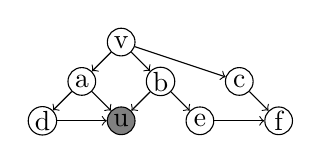
\begin{tikzpicture}[baseline=0pt]
   \begin{scope}[every node/.style={circle,draw,inner sep=0.5pt,minimum size=10pt}, treenode/.style = {circle,draw,inner sep=0.5pt,minimum size=10pt,fill=gray}]
       \node (d) at (0,0) {d};
       \node [treenode] (u) at (1,0) {u};
       \node (e) at (2, 0) {e};
       \node (f) at (3,0) {f};
        \node (a) at (0.5, 0.5) {a};
       \node (b) at (1.5, 0.5) {b};
       \node (c) at (2.5, 0.5) {c};
       \node (v) at (1, 1) {v};
   \end{scope}
   \begin{scope}[
                every node/.style={fill=black,circle},
                 every edge/.style={draw=black}]
       \path [->] (v) edge  (a);
       \path [->] (v) edge  (b);
       \path [->] (v) edge  (c);
       \path [->] (a) edge  (d);
       \path [->] (a) edge  (u);
       \path [->] (b) edge  (e);
       \path [->] (b) edge  (u);
       \path [->] (c) edge  (f);
       \path [->] (d) edge  (u);
       \path [->] (e) edge  (f);
   \end{scope}
  \end{tikzpicture}
}
	\caption{$N_G(v, 4)$.}
	
	\end{subfigure}
    \begin{subfigure}[b]{0.49\linewidth}        %% or \columnwidth
     \centering
	\resizebox{!}{!}{  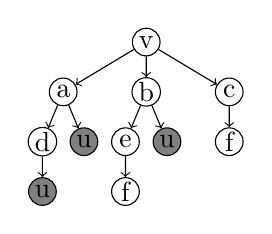
\begin{tikzpicture}[baseline=0pt,->,
  level/.style={sibling distance = 3em/#1,level distance = 1.8em},
  interestnode/.style = {circle,draw,fill=gray,inner sep=0.5pt,minimum size=10pt},
  treenode/.style = {circle,draw,inner sep=0.5pt,minimum size=10pt}]
  \node [treenode] {v}
      child{ node [treenode] {a}
               child{ node [treenode] {d}
         child{ node [interestnode] {u}}
              }
              child{ node [interestnode] {u}}
      }
      child{ node [treenode] {b}
              child{ node [treenode] {e}
         child{ node [treenode] {f}}
              }
              child{ node [interestnode] {u}}
      }
      child{ node [treenode] {c}
         child{ node [treenode] {f}
       }
     }
  ;
  \end{tikzpicture}
}
	\caption{Path-tree of $N_G(v, 4)$.}
	\label{fig:match_walks_two}
    \end{subfigure}
    \caption{左图是 $v $的一个邻域,右图由该邻域展开得到的path-tree}
    \label{fig:match_walks}
\end{figure}

图\ref{fig:match_walks}中展示了$v$的一个邻域以及它所对应的path-tree,灰色的顶点是查询顶点$u$。
path-tree中从根节点到每一个其它节点之间的路径都对应一条游走。
可以看到,这些长短不一的游走之间存在高度重合。相比于path-tree,$N_{G}(v, k)$自己本身就是一种更紧凑的存储随机游走的数据结构。
显然,我们没有显式地表示出每一条游走,那么在后面过程中必然要通过某种方式将它们表达出来。
本文采用$N_{G}(v, k)$这种数据结构有以下原因:
\begin{enumerate}
 \item 在分布式环境中,为了生成游走计算节点需要进行消息传递来获取非本地的图结构信息,
大量的随机游走需要在网络上传送。
因而使用什么样的数据结构表示它们直接关系到计算过程中的中间传输数据量,其所带来的网络开销会极大地影响算法的最终性能。
\item 因为$N_{G}(v, k)$包含了从顶点$v$出发的所有游走,那么在后续的匹配过程中,可以把邻域当做最小的匹配单位。
这意味着在分布式环境下,我们把对应于不同$v$的邻域$N_{G}(v, k)$以$v$为key分发到集群中(例如通过Spark的HashPartitioner),
剩下的匹配过程就可以在所有计算节点上分布式地并行计算,从而整个算法具有高并行度。
\item 本文在下一节会详细叙述如何基于动态规划技巧直接在邻域$N_{G}(v, k)$上进行高效地匹配计算,而无需将随机游走从$N_{G}(v, k)$重新提取出来。
\end{enumerate}

\subsection{使用动态规划技巧加速随机游走的匹配}
当$Nei$中的每个顶点$v$收集到了从它自己开始的倒序游走$N_{G}(v, k)$之后,这些从游走需要与所有的主游走$N_{G}(u, k)$进行匹配,从而计算匹配概率。
由于代表所有主游走的邻域$N_{G}(u, k)$只有很小的空间开销($O(d^k)$),我们可以把它预先广播(broadcast)到分布式集群中的每一个计算节点上。
所有的从游走$N_{G}(v, k)$按照$v$作为key被分发到不同的节点上,每个计算节点可以直接在本地进行匹配过程。
这样,算法中最耗时的匹配计算被分发到每个计算节点上进行的,使得算法具有极佳的并行性。

为了方便叙述,我们以在顶点$v$第一次相遇的随机游走为例。
我们任务是:给定主游走$N_{G}(u,k)$,在邻域$N_{G}(v, k)$中找出所有能够匹配的(主游走,从游走)对。
注意到我们只对与主游走在$v$相遇,但是之后再也不和主游走有任何共同顶点的逆序游走感兴趣。
例如,在\ref{fig:match_walks_two}中,路径$vau$和$vbe$是一对对计算$s(u,e)$有意义的匹配游走。
同理,和$vau$能匹配上的随机游走还包括$vcf$。
但是,$vad$和$vau$不是一对合法的匹配游走,因为它们首次在节点$a$而不是$v$首次相遇。实际上,
$vad$和$vau$对$s(d,u)$的计算做出了贡献,但是在分布式环境下,它们的匹配计算过程发生在$N_{G}(a, k)$所在的计算节点上。

基于以上的简单观察,可以发现以下事实:
\begin{fact}
如果我们的查询顶点$u$处于某个Path-Tree的某一层里,那么那一层的其它任一满足$LCA(u, w)=v$的顶点$w$都会点对$u,w$的相似度$s(u,w)$的计算做出
大小为$c^{l}Pr(W_u)Pr(W_w)$的贡献,其中$LCA$指的是最近公共祖先(Lowest Common Ancestor),
$W_u, W_w$是由对应Path-Tree展开的root-to-node路径。
\end{fact}
基于以上事实,我们把匹配游走这一问题看做是一个动态规划(Dynamic Programming)问题,
通过Memorization的技巧来降低匹配的时间复杂度。
对每一个$1 \leq l \leq k$,我们使用DFS算法在邻域$Nei_G(v,k)$搜索长度为$l$的匹配游走。
在DFS过程中,每一条root-to-node路径的概率被记录下来。
当DFS的深度达到$l$时,对应逆序游走的概率被保存在一个HashMap中。
当再次匹配长度为$l+1$的主游走时,就不再需要从根节点$v$开始DFS过程,因为该Path-Tree中长度小于等于$l$的逆序游走的概率之前已经全部计算过了。
例如,在图\ref{fig:match_walks_two}中,能和游走$vbdu$匹配的唯一游走是$vbef$,而计算$vbef$的概率时,我们只需要从节点$e$开始DFS过程,
因为$vbe$的概率在之前搜索$vae$的匹配游走时已经被计算过并保存了。

\begin{algorithm}[h]
\captionof{algorithm}{Dynamic Programming Path Matching}
\label{alg:dp}
\begin{algorithmic}[1]
\Procedure{LevelMatch}{$W_l, N, v, M_{l^\prime}, M_l, \delta$}
	\For {$p \in W_l$}
		\State {$br \gets$ second last vertex of $p$};
			\For {$t \in (v_N.neighbors - br)$ \& $t \notin M_l$}
				
					\If {$!M_{l^\prime}$.contains$(t)$}
						\State \parbox[t]{\dimexpr\linewidth-\algorithmicindent} {\Call{DFS}{$N, t, l, M_l,\delta, t, 1, 1$};}	
					\Else 
						\For {$w \in M_{l^\prime}$}
							\For {$nei \in w_N.neighbors$}
								\State \parbox[t]{\dimexpr\linewidth-\algorithmicindent}{\Call{DFS}{$N, nei, l,M_l,\delta,br,w.mul, l^\prime$};}
							\EndFor
						\EndFor
					\EndIf			
				
			\EndFor
	\EndFor
	\State \textbf{return} $M_l$.
	%\State \textbf{return} $results$.
\EndProcedure
\Procedure{DFS}{$N, v, l, M,\delta ,br ,mul,depth$}
	\State {$mul \gets mul * v_N.indegree$};
	\If {$mul > \delta$}
		\State \textbf{return;} \Comment{Early termination.}
	\EndIf
	\If {$depth = l$}
		\State {add $(v, mul)$ to $M(br)$};  \Comment{Record  probability.} %to the branch it resides in.}
	\Else
		\For {$nei \in v_N.neighbors$}
			\State \parbox[t]{\dimexpr\linewidth-\algorithmicindent} {\Call{DFS}{$N, nei, l, M,\delta, br,mul$, $ depth+1$};}
		\EndFor
	\EndIf
	\State \textbf{return} $M$.
\EndProcedure
\end{algorithmic}
\end{algorithm}
算法的具体细节在\ref{alg:dp}中列出。
程序LevelMatch展示了如何在邻域中寻找一个长度为$l$的主游走的所有相匹配的从游走。
各参数的意义如下:$W_l$是长度为$l$的主游走的集合;$N$是从顶点$v$开始展开的邻域;$M_{l^\prime}$ 
保存了之前调用LevelMatch函数来匹配长度为$l^\prime$主游走得到的匹配概率,具体地说它是一个(key,value)形式的HashMap,
其中key是$v$的邻居顶点,用以区分该KV元素保存的是以Path-Tree中第二层哪一个节点为根节点的子树中的信息,
value是一串元素,每个元素记录着以$key$为根节点的子树中所有游走的终止顶点及其对应的概率;
类似地,$M_l$是一个将要被填充的空的HashMap,保存匹配长度为$l$的游走的匹配概率;
最后一个参数$\delta$是一个概率阈值,其具体的含义将在下一节给出。
我们首先循环$W_l$中的每一条主游走$p$,并且知道该主游走在Path-Tree中的哪一棵子树中(第2-3行),如果$M_l$中没有记录该子树中匹配游走的概率,
就开始DFS过程(第4行)。
我们先检查$W_l{\prime}$中是否有记录该子树的信息,如果有的话就直接从记录的游走的终止节点开始调用DFS(第5-6行),
否则就需要从该子树的根节点开始DFS。
通过对所有的$W_l (l \leq k)$运行LevelMatch算法,所有游走的匹配概率都可以高效地计算出来。

\subsection{使用概率阈值剔除极小的概率}
很多现实的大图都是scale-free\cite{li2005towards}的,这意味这图中的极小比例的顶点会有极高的度数。
而我们的算法的性能与顶点的度数紧密相关,因为在生成游走过程中每条游走每经过一个度数为$d$的顶点,都会在那个顶点分裂为$d$条更长的游走。
因此,我们使用一个阈值\cite{lizorkin2008accuracy}$\delta$来删除那些包含多个拥有极高度数的顶点的游走,
因为根据公式\ref{eq:seven},这些游走的概率非常之小,对最终计算精度的影响基本可以忽略不计。
$\delta$的使用展示在算法\ref{alg:dp}的14-15行。
$\delta$的具体取值应在算法的精度与时间、空间复杂度之间取得平衡,更大的$\delta$意味着更低的精度,但是算法
整体的时间复杂度和空间复杂度更低,反之反是。
\subsection{算法的复杂度分析}
源点$u$可达的顶点数目大约为$O(d^k)$,
而对于其中的每一个可达顶点,都拥有一个大小为$O(d^k)$,隐式包含$O(d^k)$条逆序游走信息的邻域,
因此,总的空间复杂度为$O(d^{2k})$。因为这个过程中所有产生的游走都需要通过网络传输,所以通信开销也是$O(d^{2k})$。
在对游走进行匹配时,对每一个邻域,大约有$O(d^k)$个游走被匹配了,所以总的计算复杂度为$O(d^{2k})$。
可以看到,算法总的复杂度与整个图的规模$O(n+m)$没有依赖关系。
\section{基于Spark平台的算法实现}
基于Spark平台的算法实现可以概括为4个步骤:
\begin{enumerate}
 \item 找出从顶点$u$出发顺着入边经过$k$步可达的邻域$Nei$,同时记录所有的主游走。然后将所有的主游走广播到集群所有计算节点上。
 \item 从$Nei$中每一个顶点$v$出发,顺着出边找出其$k$步可达的邻域,这些邻域看做一个以$v$为key的key-value对,分发到集群中。
 \item 将上面每一个$v$的邻域和第一步中的$Nei$进行匹配,计算相遇概率。这一过程是分布式的。
 \item 聚合所有的相遇概率得出最终的相似度$s(u,*)$。
\end{enumerate}
上述四个步骤中第1个和第2个很相似,区别只是要获得邻域的顶点的数量(1 vs $|Nei|$)。
因此我们重点描述第2、 3、 4步骤在Spark平台上的实现。

我们首先将表示图的原始文本数据上传至分布式文件系统HDFS上,然后Spark读入图数据,生成对应的RDD。
在计算过程中,由于需要迭代计算,所以需要使用Spark提供的cache机制将RDD内容缓存在内存中,这样可以极大地提高迭代计算的效率。
计算过程还需要使用Spark的broadcast机制将所有主游走广播到集群中每一个计算节点上。broadcast适合传输规模小、不会改变的数据。
\subsection{邻域收集步骤}
\begin{algorithm}[h]
\captionof{algorithm}{Collect Neighborhood}
\label{algo:nei_collect}
\begin{algorithmic}[1]
	\Procedure{Collect}{$edgeRDD, Nei, k$}
		\State {$graphRDD \gets edgeRDD$}
		\State {\qquad .{\asciifamily reduceByKey}$()$.{\asciifamily cache}$()$};
		\State {$nbrhdRDD \gets graphRDD$.{\asciifamily map}$()$.{\asciifamily cache}$()$};
		\State {$nbrRDD \gets graphRDD$.{\asciifamily filter}$()$.{\asciifamily cache}$()$};
		\For{$ l =2$ to $k$}
			\State {$nbrRDD \gets  nbrRDD$}
			\State {\qquad.{\asciifamily join}$(graphRDD)$.{\asciifamily map}$()$};
			\State {$nbrhdRDD \gets nbrhdRDD$}
			\State {\qquad .{\asciifamily leftOuterJoin}$(nbrRDD)$.{\asciifamily map}$()$};
		\EndFor
	\State \textbf{return} $nbrhdRDD$.
	\EndProcedure
\end{algorithmic}
\end{algorithm}
算法\ref{algo:nei_collect}展示了生成邻域的具体细节。
算法总共接受3个参数:$edgeRDD$表示从HDFS读入的、每个元素代表图中一条边的RDD,$Nei$是要生成邻域的出发顶点集合,$k$是游走的最大长度。
首先我们把图从按照边存储的格式变为邻接表这种格式,并存储在$graphRDD$中(第2-3行),
然后我们从$graphRDD$生成$nbrhdRDD$(第4行),这个RDD里面存放着所有的邻域。
$nbrRDD$表示所有邻域的最外面一层,初始化时它就是集合$Nei$的直接邻居顶点(第5行)。
接下来算法以迭代方法不断纳入新的边来对$nbrhdRDD$进行扩张,即把之前邻域最外围的顶点$nbrRDD$的邻居节点纳入到邻域中。
每一次扩张也代表着游走的最大长度增加了一步,这个操作是通过Spark中的连接(join)操作完成的。
每次扩张时通过$nbrRDD$与$graphRDD$做连接操作得到最新的最外围顶点(第7-8行),
再通过$nbrhdRDD$与$nbrRDD$做连接操作把这些顶点纳入到邻域中(第9-10行)。

\subsection{匹配游走步骤}

\begin{algorithm}[t]
\captionof{algorithm}{Compute SimRank}
\label{algo:match}
\begin{algorithmic}[1]
\Procedure{Compute}{$nbrhdRDD, MW,  u, k$}
	\State {$simRankRDD \gets hbrhdRDD$}
	\State {\qquad .{\asciifamily flatMap}$((v, nbrhd) \Rightarrow\{$}
	\State {\qquad \qquad create $MP$};
	\State {\qquad \qquad \textbf{for} $W_l$ in $MW$ \textbf{do}}
	\State {\qquad \qquad \qquad $M \gets$ \Call{LevelMatch}{$W_l, \dots $}};
	\State {\qquad \qquad \qquad extend $MP$ with all elemetns in $M$};
	\State {\qquad \qquad \textbf{for} $(v, score(u,v))$ in $MP$ \textbf{do}}
	\State {\qquad \qquad \qquad yield $(v, score(u,v))$};
	\State {\qquad $\})$}
	\State {$s(u,*) \gets simRankRDD$.{\asciifamily reduceByKey}$()$.{\asciifamily collect}$()$};
	\State \textbf{return} $s(u, *)$.
\EndProcedure
\end{algorithmic}
\end{algorithm}


当所有邻域全部生成完毕后,我们开始匹配主游走和从游走。具体细节如算法\ref{algo:match}所示。
程序接受4个参数:$nbrhdRDD$表示算法\ref{algo:nei_collect}的返回结果;$MW$表示被广播到集群各个计算节点上的所有主游走,
其数据结构是一个由$key-value$对组成的HashMap,其中$key$是每个主游走的终止顶点(因此$key \in Nei$),
$value$是所有以$key$终点的随机游走;剩下两个参数$u$和$k$分别是查询节点和游走的最大长度。
对$nbrhdRDD$中的每个元素$(v,nbrhd)$,我们调用算法\ref{alg:dp}计算$nbrhd$中所有游走的相遇概率。
注意到$nbrhdRDD$中的所有元素以$v$为$key$被Spark默认的Partitioner均匀分布在集群中,因此整个计算过程是分布式的。
计算出的结果被组装成一个列表(第7行),然后经flagmap操作发射出去(第8-9行),
最后经由reduceByKey操作将属于不同$v$的相似度$s(u,v)$聚集起来,并送至Driver Program(第11-12行)。

	

\section{实验评估}
本章使用真实的数据集综合评定算法的性能,主要的考察点包括:算法的有效性,计算结果的收敛性质,参数对算法效率的影响,算法的计算效率和算法的可扩展性。
\subsection{实验环境}
集群包括6个计算节点,每个节点处理器为12核的Intel Xeon E-2650,频率为2.1GHz,
内存为64GB,硬盘为1TB。 节点之间由千兆网卡连接。操作系统为Ubuntu 16.04。 
Spark运行版本为1.6.2, 底层分布式文件系统HDFS的版本号为2.6.0。
所有的节点都配置为slave节点,其中一个节点被额外配置为master节点。 
在Spark运行时,我们为每个executor分配10GB内存。
\subsection{实验数据集}
我们一共使用了5个真实的图数据来评估算法的性能。 数据集的具体细节如表\ref{tab:dataset1}。
其中,p2p-gnutella08是一个P2P文件分享网络的结构;
wiki-vote是一个反映维基百科用户竞选社区管理者而相互投票情况的数据;
eu-2005是一个从.eu域名爬取的小部分网页链接数据;
ljournal-2008是一个虚拟社交网络。
每个图初始时为普通的文本格式,每一行代表图中的一条边。
在开始实验前,所有的数据集都预先上传到分布式文件系统HDFS上。
\begin{table}[h]
\caption{数据集描述}
\label{tab:dataset1}
\centering
\begin{tabular}{|l|r|r|r|r|}
\hline
\textbf{数据集} & \textbf{顶点数} & \textbf{边数} & \textbf{顶点平均度数} & \textbf{大小} \\
\hline
p2p-gnutella08 \footnotemark[1]  & \num{6301}         & \num{20777}                   & \num{3.29}               & \num{215.2}KB\\
\hline
wiki-vote \footnotemark[2]    & \num{7115} 	& \num{103689}                           &\num{14.57 }              & \num{1.1}MB  \\
\hline
%wiki-talk            & \num{2394385} & \num{5021410}          &2.10                   & 66.5MB\\
%\hline
eu-2005       \footnotemark[3]     & \num{862664}  & \num{19235140 }          & \num{22.29}             & \num{256.4}MB\\
\hline
ljournal-2008  \footnotemark[4] & \num{5363260} & \num{79023142}         & \num{14.73}            &\num{1.2}GB\\
\hline
arabic-2005 \footnotemark[5]   & \num{22744080} & \num{639999458}      & \num{28.14}           & \num{10.9}GB\\
%\hline
%twitter-2010    & \num{41652230 } & \num{1468365182} & 26.1GB\\
\hline
\end{tabular}
\end{table}
\footnotetext[1]{https://snap.stanford.edu/data/p2p-Gnutella08.html}
\footnotetext[2]{https://snap.stanford.edu/data/wiki-Vote.html}
\footnotetext[3]{http://law.di.unimi.it/webdata/eu-2005/}
\footnotetext[4]{http://law.di.unimi.it/webdata/ljournal-2008/}
\footnotetext[5]{http://law.di.unimi.it/webdata/arabic-2005/}
\subsection{实验参数设置}
根据文献\cite{lizorkin2008accuracy}中的描述,通常算法所需要的最大迭代次数$k$是由衰减系数$c$和最终结果所要求的精度决定的。 
如果希望最终误差 $s^*(u,v) - s^k(u,v)$小于某个$\epsilon$,那么$k$至少要被设置为$k=\lfloor \log_c \epsilon \rfloor$。
在我们的实验中,我们选取$\epsilon=0.01$,因为这样的精度可以满足大多数实际应用。 
$c$被设置为0.5,相应地,$k$被设置为$k=6$。
此外,用于过滤掉极小概率的游走的阈值被设置为$\delta=0.002$。注意到这里的$\delta$指的是一个随机游走的概率阈值,
根据公式\ref{eq:five},对于一对匹配好的游走,其对应的匹配概率相应的阈值变成${\delta}^2$。
如果再考虑到因子$c^l$,那么这个概率是极端小的,完全可以忽略。

算法精度的测试方法是多次实验取平均值,每次实验时随机选取图中的某个顶点为查询顶点。
对于小图(大小<10MB),我们重复实验1000次计算其平均值;对于更大的图,重复次数设为10000。
\subsection{算法有效性}
\begin{figure}[h]
\centering
\begin{subfigure}[b]{0.48\textwidth}
	\center
	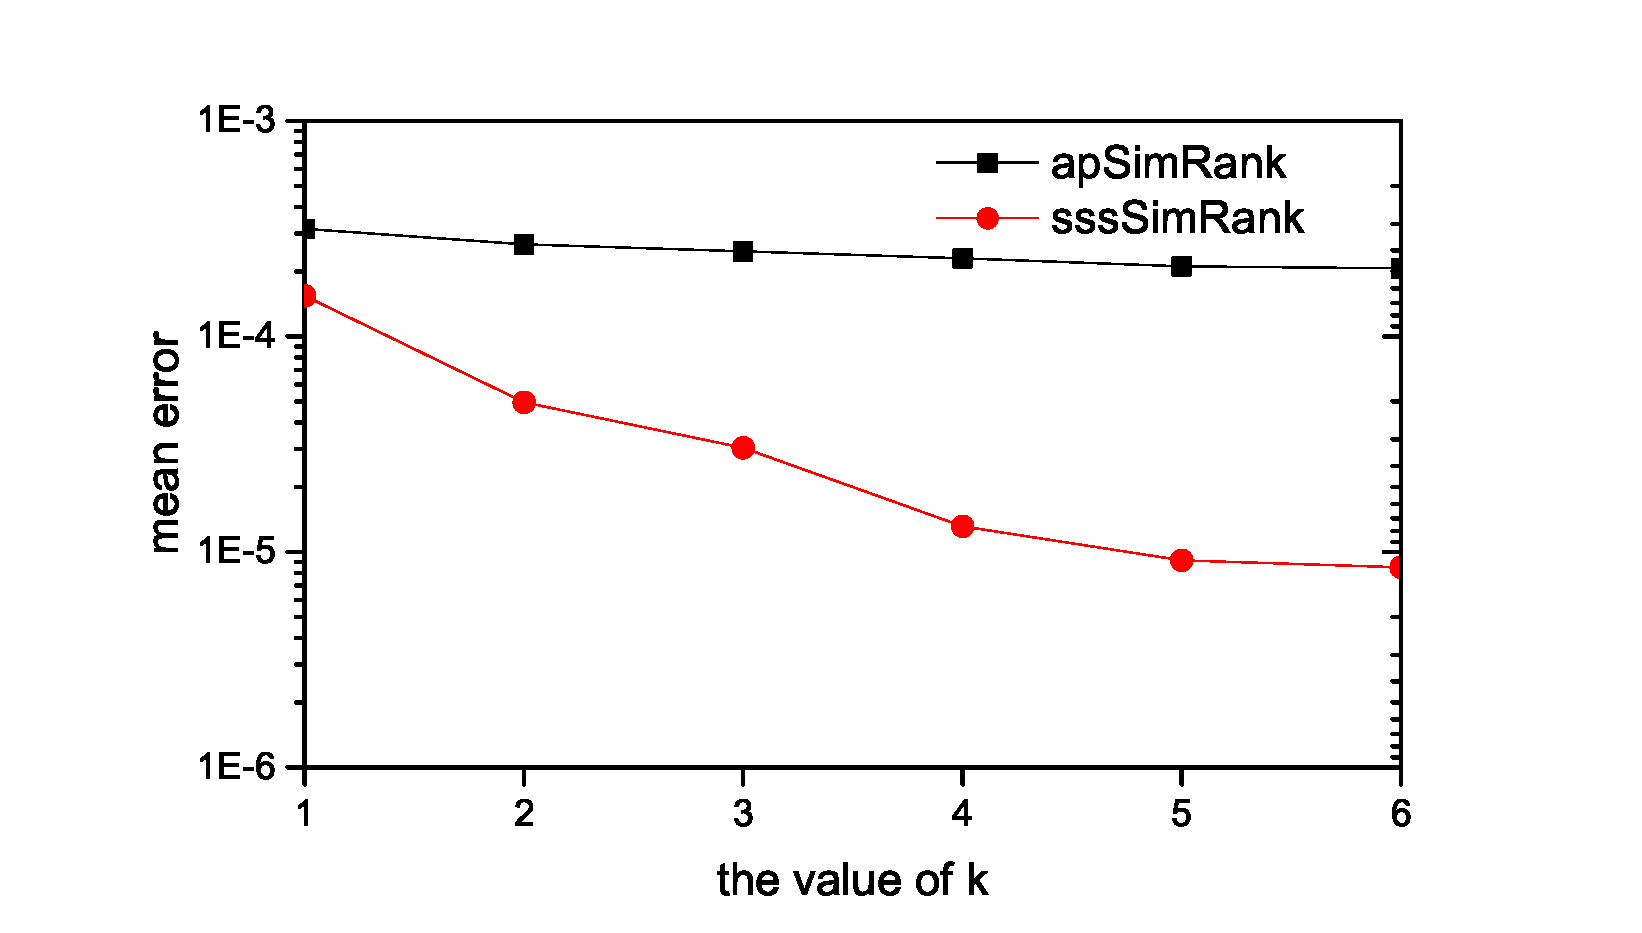
\includegraphics[width=1\textwidth]{figure/accuracy1.eps}
	\caption{p2p-gnutella08}
	\label{fig:ch1:effec:one}
\end{subfigure}
\begin{subfigure}[b]{0.48\textwidth}
	\centering
	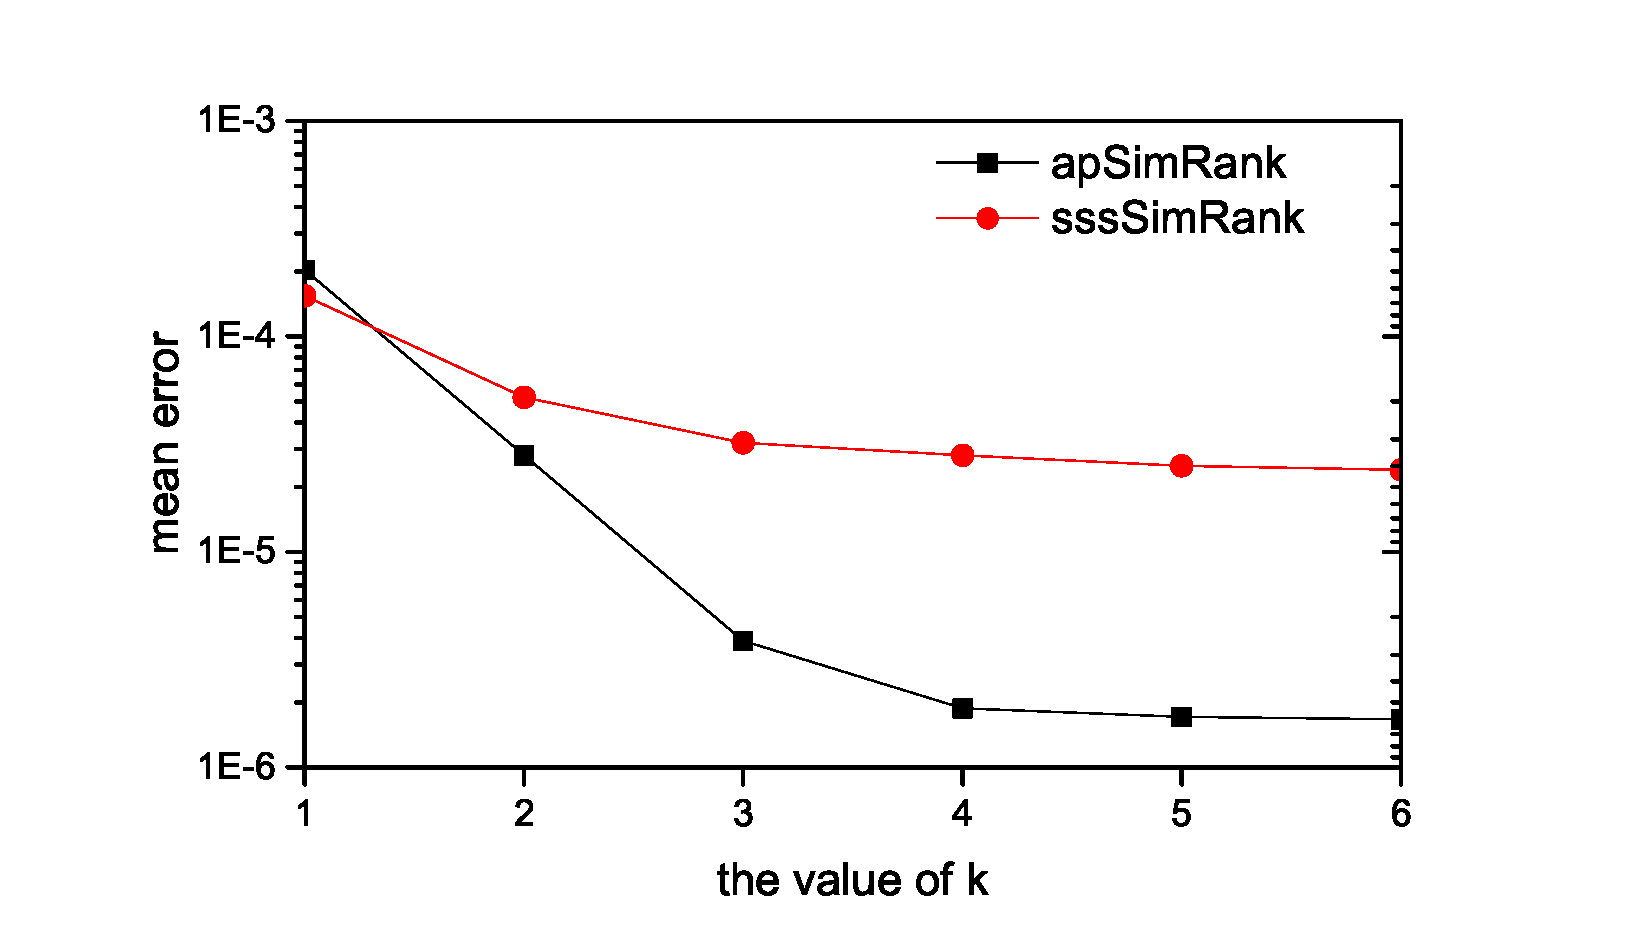
\includegraphics[width=1\textwidth]{figure/accuracy2.eps}
	\caption{wiki-vote}
	\label{fig:ch1:effec:two}
\end{subfigure}
\caption{标准计算方法和sssSimRank的相似性误差随迭代次数的变化曲线比较}
\label{fig:ch1:effect}
\end{figure}
首先比较我们的算法sssSimRank和标准计算方式apSimRank的时间收敛速度。
选取的误差指标为平均误差(mean error),即$ME = \frac{1}{n}\sum_{v \in V}{\left|s(u,v) - s^k(u,v)\right|}$,
其中$s(u,v)$为根据公式\ref{eq:two}迭代计算至完全收敛的真实相似性,$s^k(u,v)$为我们算法迭代$k$次后的相似性。
我们在两个小图上进行实验。其中p2p-gnutella08是个比
较稀疏的图,平均顶点度数$d=3.29$;而wiki-vote是一个更加稠密的图,平均顶点度数为$d=15.57$。
图\ref{fig:ch1:effect}为最终的比较结果。
从图中可以看到,二者在6次迭代以内精度都得到了收敛, 我们的算法sssSimRank有更好的收敛速度,三次迭代之后平均误差就在$10^{-4}$以内。
这是因为我们的算法“抓大放小”剔除了小概率游走,而apSimRank仍然需要继续计算它们。
另一个现象是在图\ref{fig:ch1:effec:one}中sssSimRank的平均误差与apSimRank的差距比图\ref{fig:ch1:effec:two}更小,
这是因为我们的算法中使用了概率筛除的缘故。对于同一个概率阈值$\delta$,图的平均顶点度数越大,则小概率游走越多, 相应地,被剔除的小概率游走越多,
所以对最终精度的影响越大。 
本质上,$\delta$的作用是牺牲一定的精度来换取计算效率的提高。
即便如此, sssSimRank的相似性误差仍然非常小($<10^{-4}$), 完全可以满足大部分应用的精度需求。
\subsection{算法的效率}
为了比较算法的运行效率,我们分别基于Spark平台实现了分布式的全点对算法apSimRank, 算法\ref{algo:nssSimRank}所示的nssSimRank,以及本文提出的算法sssSimRank。
直接比较这三个算法的运行时间非常困难,因为apSimRank以及nssSimRank实际运行非常耗时,
在规模最小的图p2p-gnutella08上, apSimRank需要运行2.1个小时才能完成计算,而nssSimRank需要计算1.2个小时。
因为对于基于随机游走模型的算法而言,其运行效率主要取决于所生产的随机游走的数量,进一步地说,取决于需要从多少个邻域$Nei$来展开生成随机游走。
因此,我们比较sssSimRank和nssSimRank算法中生产$Nei$的数量。结果如图\ref{fig:ch1:runtime}所示。
\begin{figure}[h]
  \centering
  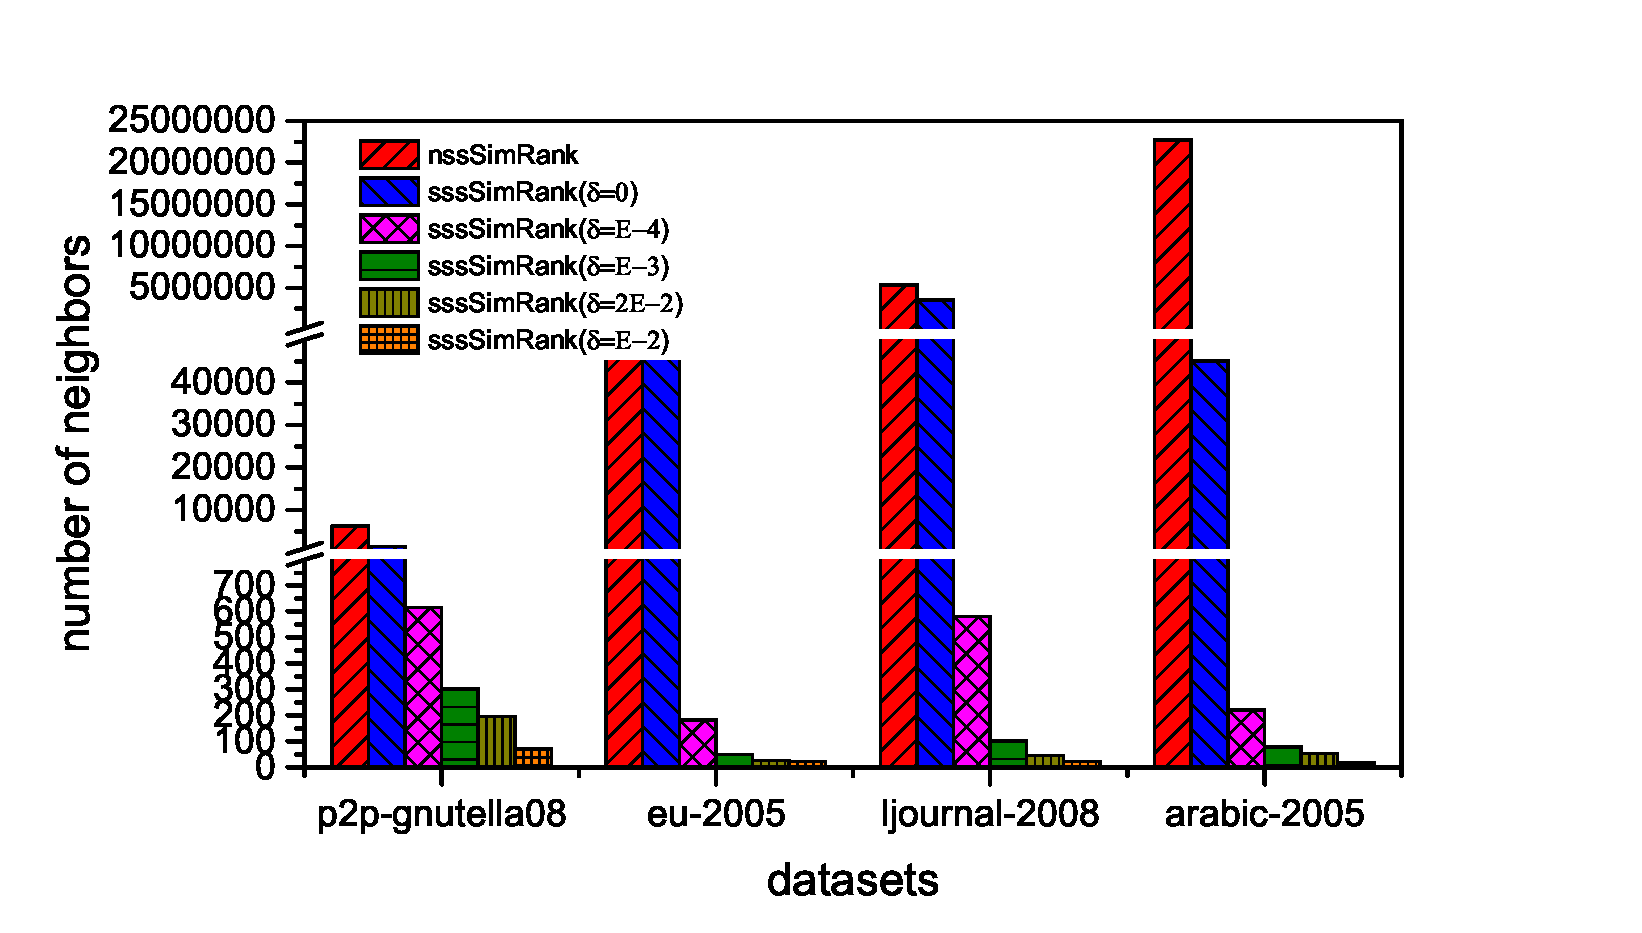
\includegraphics[width= 1\textwidth]{figure/neighborhoods.eps}\\
  \caption{生成邻域数量的比较}\label{fig:ch1:runtime}
\end{figure}
从图中可以看出,sssSimRank极大地减少了生成邻域的数量。
当$\delta=0$时,即算法没有筛除概率极小的游走时,邻域数量减少了大约1500x倍。
从图中还可以观察到邻域数量与概率阈值$delta$之间的关系。
当$\delta$越来越大时,意味着概率“筛子”的“孔”变得越来粗,幸存的随机游走会越来越少。
图\ref{fig:ch1:runtime}还表明,我们的算法在数据集eu-2005和arabic-2005减少邻域的比例比图p2p-gnutella08和ljournal-2008要大很多,
这一观察同样表明算法中的概率筛子对稠密的图能更好地提高性能。
\subsection{算法的可扩展性}
我们考察分布式环境下算法的可扩展性。 首先考察算法运行时间随着输入图的大小的变化关系,结果如图\ref{fig:ch1:data_scalable}所示。
图中展示了当集群计算节点数目固定时,对于不同的$\delta$,运行时间随输入图规模大小变化的情况。 
可以看出,输入图的规模从215KB增长到10.9GB,而对应的运行时间基本上近似的随着输入规模大小线性的变化,
这一结论对不同的$\delta$都成立。这展示出sssSimRank良好的数据可扩展性。
\begin{figure}[h]
  \centering
  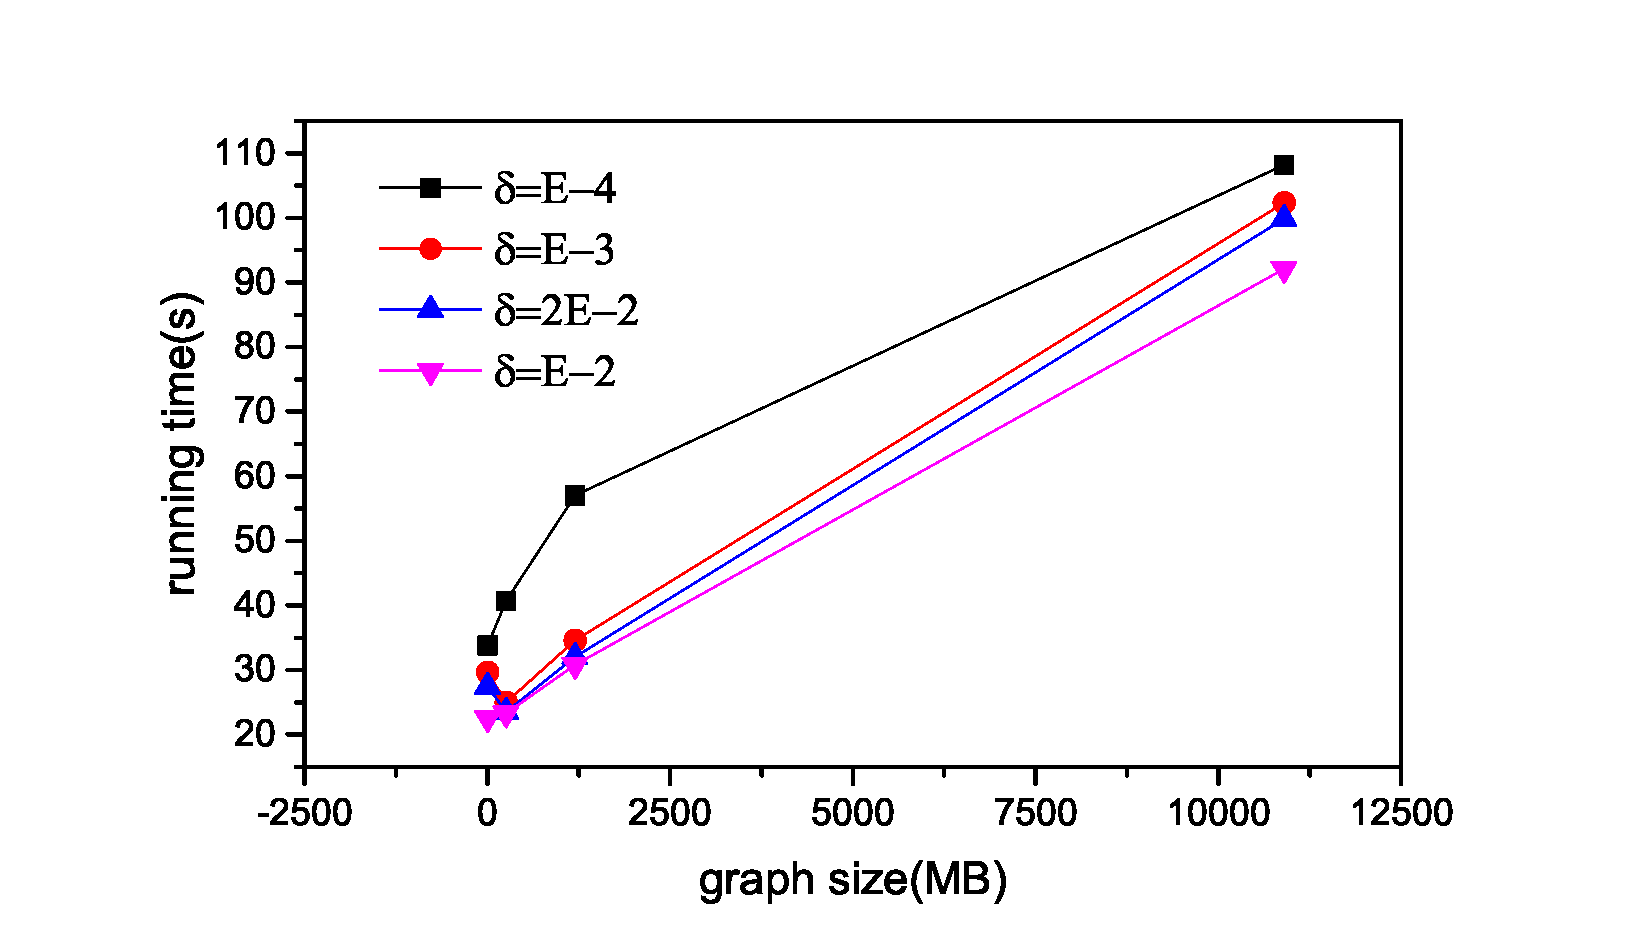
\includegraphics[width= 1\textwidth]{figure/data_scalability.eps}\\
  \caption{算法运行时间与输入图大小的变化关系}\label{fig:ch1:data_scalable}
\end{figure}

我们还考察了当输入图的规模固定时,算法运行效率随集群中计算节点数量变化的情况。
所有的输入图使用同样的参数配置,$k=6$, $\delta=10^{-4}$。 计算节点数量从2增加到6。
注意到我们把$\delta$取得非常小,是因为$delta$越小,算法剔除的游走越少,总的计算量越大,
这样更能体现计算量较为饱和的情况下算法的节点可扩展性。实验结果如图\ref{fig:ch1:node_scalable}所示。
从图中可以看到,对不同规模的输入图,算法的运行时间随集群计算节点的增加而近乎线性的减少,
这表明我们的分布式计算方法具有良好的节点可扩展性。
\begin{figure}[h]
  \centering
  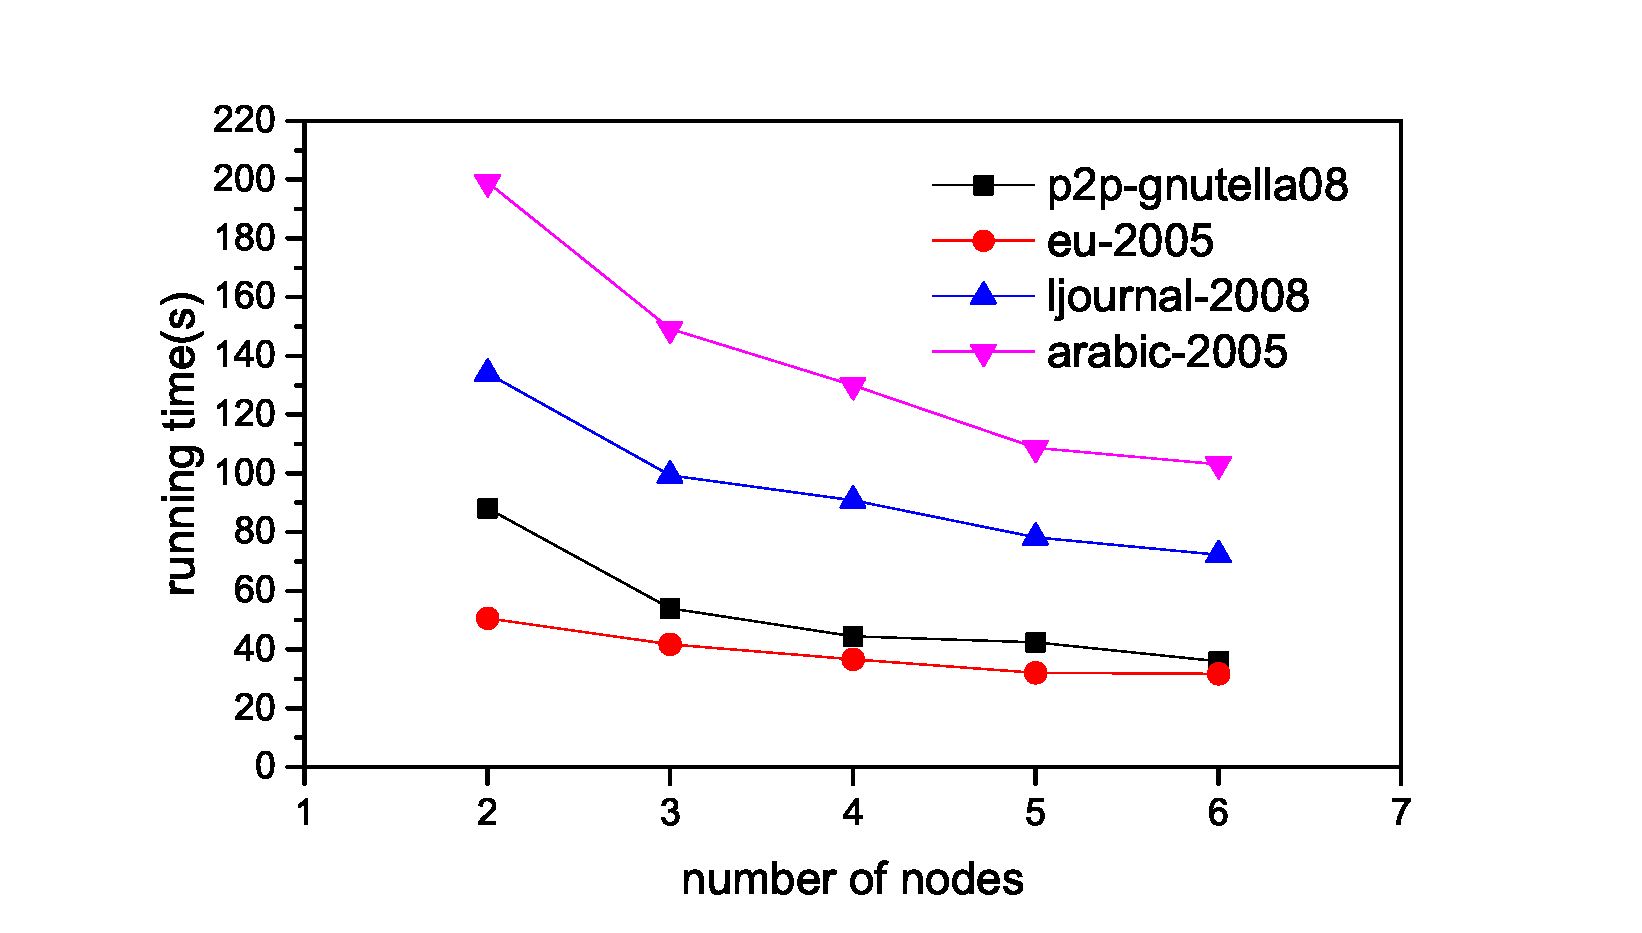
\includegraphics[width= 1\textwidth]{figure/node_scalability.eps}\\
  \caption{算法运行时间与集群计算节点数量的变化关系}\label{fig:ch1:node_scalable}
\end{figure}

\section{本章小结}
本章针对图数据中单源点SimRank相似度计算问题,提出了一种基于随机游走的分布式算法。
整个算法包含三个步骤:首先生成随机游走,再对游走进行匹配计算其对应概率,
最后汇总得出相似度。
针对计算本身的高时间复和空间复杂度,本文设计了一系列方法来提高计算效率,包括减少随机游走的数量,使用更紧凑的数据结构来压缩中间数据,以及通过动态规划
的技巧加速随机游走的匹配计算。
本章给出了算法在Spark平台上的实现,基于真实数据的实验结果验证了算法的计算效率、有效性和可扩展性。
%%%%%%%%%%%%%%%%%%%%%%%%%%%%%%%%%%%%%%%%%%%%%%%%%%%%%%%%%%%%%%%%%%%%%%%%%%%%%%%
\chapter{基于模块度优化的分布式图划分方法}\label{chapter_graphpartition}
\section{概述}
随着现实生活中数据规模的不断扩大,与之对应的图数据网络结构愈加复杂,规模也不断增大,典型的大图甚至有数十亿个顶点和上万亿条边。
普通的单台计算机由于运算内存的限制,远远无法胜任对大规模图数据的计算处理任务,
这给解决一些基于图计算的常见问题(如寻找连通分量\cite{DBLP:conf/sc/HongRO13}、
计算三角形\cite{DBLP:journals/corr/abs-1011-0468}、计算PageRank\cite{page1999pagerank}、
计算SimRank\cite{jeh2002simrank}等)带来了巨大的挑战。
因此,首先将图划分成多个子图装载到不同计算节点上中,然后再充分利用分布式平台进行后续的图分析、图信息挖掘任务,
是处理大规模图数据唯一可行的方案。

图划分按划分对象归类为为两类:切分边(edge cuts)和切分顶点(vertex cuts)。
前者以顶点为最小单位进行划分,划分后图中的一条边的两个端点可以处于不同的分块中;
后者以边为最小单位进行划分,划分后同一个顶点可以出现在多个分块中的多条边中。
图\ref{fig:partition_scheme}展示了两种不同的方法。
\begin{figure}[h]
  \centering
  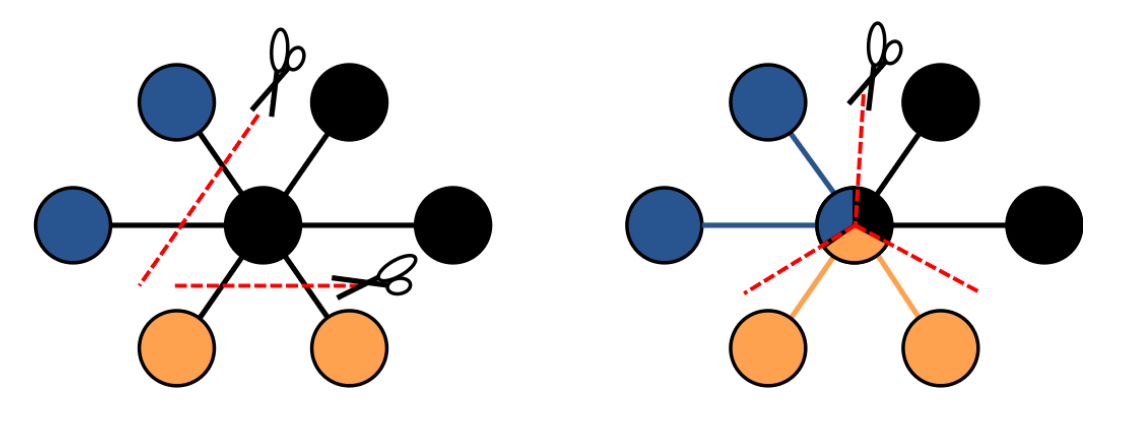
\includegraphics[width= 0.7\textwidth]{figure/partition_approach.png}\\
  \caption{两种划分方式。左图以顶点为基本划分单位,右图以边为基本划分单位}
  \label{fig:partition_scheme}
\end{figure}
这两种划分方法有各自适用的场景\cite{DBLP:conf/eurosys/ChenSCC15}:对于绝大多数顶点度数都很低的图,前者更合适,因为顶点存放在本地的邻接表规模较小;
而对于有很多极高度数的顶点的图,后者是更合适的选择,因为与这些顶点相关的计算可以分发到不同计算节点上去实现负载均衡。
本文关注以边为对象的划分方式,如无特殊说明,本文下面提到的图划分都是指对图中顶点的划分。

图划分问题可以用数学语言描述如下: 给定一个图$G(V, E)$,图的划分即将$V$划分为$k$个子集$(C_1, C_2, \dots, C_k)$,
使得对任意$1 \leq i,j \leq k$,满足下列约束:
\begin{equation}
\begin{aligned}
\label{eq:4-1}
 C_i \cap C_j=\emptyset \\
 \bigcup\limits_{i=1}^{k} C_{i} = V
 \end{aligned}
\end{equation}
通常,图划分问题往往还需要满足其它的约束条件,例如每个子集$C_i$的大小需要满足一定限制。
给定一个划分,两个端点分别处于不同子集的边的权重(或数量)称作边割(edge-cut)。
边割的大小揭示了划分是否最大程度地保留了原图中的稠密子结构,是衡量最终划分结果质量的重要标准,
通常图划分的目标函数里需要以某种形式最小化边割的大小。

作为图论领域的经典问题,目前已经有大量的工作对图划分做了各式各样的研究。 
文献\cite{garey1974somenp}证明,图划分是一个NP完全问题,通常无法在可接受的时间范围内找到其理论上的最优解。
对于大规模图数据而言,将图中的顶点划分为不同的分块并将其存储到集群中不同的计算节点上去,
这一过程中每个计算节点为了能够访问到非本地存储的拓扑信息,必然会产生网络开销。
因此,采用什么样的方法对图分割,对划分过程中的网络开销、分配均衡、划分质量有着决定性影响。
对超大规模图而言,其划分任务面临着新的挑战:
\begin{enumerate}
\item 算法需要有极好的可扩展性,这要求算法本身能够充分发掘划分过程的计算可并行性,可以通过堆砌计算节点获得更大的处理能力;

\item 划分结果需要较好地保留原图的语义。
现实生活中的图并不是随机生成的,它们的拓扑结构往往隐含着语义(semantic)层面的信息。好的划分算法应当尽量保留图中的语义信息。
\end{enumerate}

因而设计一个好的分布式图划分方法具有重要的显示意义。
针对以上问题,我们提出一种高效的分布式图划分算法,实验结果表明,该方法具有较高的效率以及较好的可扩展性。

\section{相关工作}
目前学术界对图划分问题做了大量的研究,概括地说,目前的划分方法主要有以下几种:

\textbf{单节点串行算法。 } 文献\cite{garey1974somenp}证明了图划分问题是一个NP完全问题。 
因此,早起很多工作都集中在设计一些近似算法以求得次优解。
文献\cite{kernighan1970efficient}提出了Kernighan-Lin(KL)算法,该方法首先将图初始划分为偶数个分块,
然后基于一些启发式信息不断交换不同分块中的顶点,直到不同划分之间的边割($edge-cut$)的权重之和达到最小。
KL算法每次迭代的时间复杂度为$O(n^3)$,它的划分质量较高,但是不能应用在超图(supergraph)上,而且对于规模稍大的输入图就显得无能为力。
FM算法\cite{fiduccia1988linear}改进了KL算法中的顶点交换策略,每次不再交换一堆顶点而是改为基于分割线使得顶点在分割线两侧移动。
顶点移动的标准是最大化划分的负载均衡度。FM算法的适用范围扩展到了超图,它的每次迭代拥有线性的时间复杂度。
还有一些基于模拟退火\cite{johnson1989optimization},遗传算法\cite{bui1996genetic}的解决方案。
这些方法的研究对象都是基于单节点内存存储的小图。

为了能够应对更大规模的图,一些多层次划分的方法相继被提出,包括 Metis\cite{Karypis95metis},Chaco\cite{leland1995chaco}
和Scotch\cite{pellegrini1996scotch}。
这些方法主要由三个步骤组成:图的塌缩(coarsening phase)、初始划分(initial partition phase)、恢复(uncoarsening phase)。
其中,塌缩是指将图中若干顶点变为一个顶点,同时减少边的个数,从而提取出整个图拓扑信息的“骨骼”并基于此构造一个更小的图; 
初始划分指的是经过多次塌缩过程后,在得到的小图上运行传统图划分算法得到一个原始划分;
最后恢复过程按照塌缩步骤的相反顺序逐渐将图恢复成原来的形状,将原始划分投影成原输入图上的最终划分。
这三个阶段缺一不可, 共同完成了从大规模图数据到简单小图再重新恢复的过程。
尽管可以处理的图规模有所扩大,目前这些软件包可接受的输入数据依然都是基于单节点存储的小图。

\textbf{单节点并行算法。 } 为了进一步充分利用现代CPU的多核特性,从以上这些单线程算法中演化出一些并行化算法,
典型的有ParMetis\cite{karypis1998parallel},Pt-Scotch\cite{chevalier2008pt}等。 
这些算法或多或少地挖掘出图划分问题本身潜在的计算可并行性,所以其能够处理的图的规模也获得了的提升。 
但总的来说这些方法仍然是基于单计算节点的,其计算能力受到有限的计算资源的限制,对规模更大的(上百万节点)图无能为力。

\textbf{分布式图划分。 } 近年来,一些专门用于图计算的分布式平台越来越流行,包括Pregel\cite{malewicz2010pregel},
Spark GraphX\cite{DBLP:conf/osdi/GonzalezXDCFS14}, Trinity\cite{shao2012trinity}等等。
这些平台的一个典型特点是支持以顶点为中心(vertex-centric)的编程范式,并且在系统层面拥有原生的顶点间消息通信机制。
然而上面几个流行的平台尽管也开放了一些接口支持用户按照需求设计自己的划分方法,但都没有提供一个直接可用的、高效的分布式图划分方法。
在读入输入数据时,它们往往使用随机划分的方法加载图数据,其划分质量没有任何保障。
以GraphX为例,它提供了几种简单的以边为划分对象的划分机制:EdgePartition2D, EdgePartition1D, RandomVertexCut,CanonicalRandomVertexCut。
第一种方式对图的邻接矩阵进行二维的划分,例如对9$\times$9的矩阵,将其均匀划分成9个3$\times3$的分块,再把这些分块划分到集群中的9个节点上去。
剩下三种方式都是按照边的两个端点的ID信息进行哈希从而将边划分到不同节点中去。

\textbf{流式图划分。} 文献\cite{DBLP:conf/wsdm/TsourakakisGRV14}\cite{DBLP:conf/kdd/StantonK12}研究了流式图的划分方法。
这种场景下图中的顶点以数据流的形式流入系统,算法无法感知图的全局拓扑结构。这类方法使用一些简单的局部启发式信息对图进行划分,因而划分质量往往不是最优。

\section{算法的基本框架}
我们从以下两方面来考虑图划分算法的优化目标:
\begin{enumerate}
 \item 划分结果顶点的分配均衡。 理想情况下,每个分块中顶点的数目应该尽可能相似。 
 如果用$bs$表示分块中顶点数目的上限,那么对划分$P=(C_1, C_2, \dots, C_n)$,应该有$\max\limits_{i}|C_i| \leq bs$。
约束条件$bs$的设置可以与具体情景有关,比如集群中计算节点的内存容量一定满足是$bs$的一个上限。
 \item 划分结果的质量。 理想情况下图划分算法应该可以把图中稠密的子图归类于一个分块中。
 但是图中稠密子图的规模天然是不均匀的,而划分过程中有负载均衡的限制,因此我们需要从整体考虑划分的质量。
 设$P$是图$G(V,E)$的一个划分,定义其边割(edge-cut)为
 $EC =\sum\nolimits_{e(u,v) \in E, u \in C_i, v \in C_j} w\big(e(u,v)\big)$,即所有连接不同分块的边的权重之和。
 理论上,$EC$应尽可能的小。
\end{enumerate}
我们的算法借鉴多层次划分(Multi-Level Partitioning)的思想,主要有下面三个步骤:
\begin{enumerate}
 \item 首先不断地通过塌缩步骤使原图的规模越来越小。
每次进行塌缩时,先对图做效果有限的简单划分,然后将划分结果的每一个分块当做一个新的顶点,分块之间的边当做一条新的边,形成一个规模小很多的图。
\item 经过多次迭代塌缩后,图的规模小到某个可以接受的阈值,再使用KL或FM等传统高质量单节点算法直接进行划分,得到初始划分的结果。
\item 最后将初始化分划直接投影到原图中,这样就得到了最终的划分结果。
\end{enumerate}
图\ref{fig:mlp_framework}揭示了多层次划分算法的大致框架,每一步的具体细节将在下文给出。

\begin{figure}[th]
  \centering
  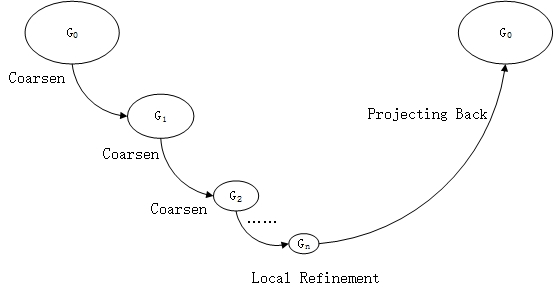
\includegraphics[width= 0.75\textwidth]{figure/coarsen.jpg}\\
  \caption{多层次图划分的算法框架}
   \label{fig:mlp_framework}
\end{figure}

\subsection{塌缩步骤}
设原始输入图为$G_{0}(E_0,V_0)$,迭代塌缩过程中产生的中间图由记号$G_1, G_2, \dots, G_t$表示。
相应地,由中间图产生的划分表示为$P_1, P_2, \dots, P_{t}$。
注意到迭代过程中图的划分与其输入图下标是对应的,即$G_{i-1} \rightarrow P_i \rightarrow G_i$。
我们首先给出塌缩的具体过程。
\begin{definition}
塌缩图的拓扑结构。 迭代塌缩过程中,给定图$G_i(V_i, E_i)$上的划分$P_i=(C_1, C_2, \dots, C_n)$,基于$P_i$上构造塌缩图$G_{i+1}(V_{i+1}, E_{i+1})$如下:
 令$V_{i+1} = P_i$,即$P_i$中的每一个划分对应$G_{i+1}$中的一个新顶点;边$(C_i, C_j) \in E_{i+1}$当且仅当$\exists
 u \in C_i, v \in C_j$ 并且 $(u, v) \in E_i$。
\end{definition}
通过这样的塌缩过程,显然有$|V_{i+1}| < |V_i|$,也就是说图的规模在迭代中不断变小。
经过反复塌缩后,图$G_i$的规模会降低到某个阈值以下。
\begin{definition}
塌缩图的权重。 设初始输入图$G_{0}(V_0,E_0)$中每个顶点有单位权重$w_u=1$,每条边$(u,v)$同样有单位权重$w_{u,v}=1$。
设迭代过程中基于图$G_i$构造塌缩图$G_{i+1}$,并且有$V_{i+1}=(C_1, C_2, \dots, C_n)$,
那么新的图中顶点$u$的权重定义为:
\begin{equation}
\label{eq:vertex_weight}
w(u) = \sum\limits_{v \in C_k} w(v)
\end{equation}
其中,$C_k$为图$G_{i+1}$中新顶点$u$在图$G_i$中对应的分块。
类似地,边$e=(C_i, C_j)$的新权重定义为:
 \begin{equation}
w(C_i, C_j) = \sum\limits_{(u,v) \in E_i, u \in C_i, v \in C_j} w(u,v)
\end{equation}
即塌缩图中的新顶点的权重为原图中对应分块中的所有顶点的权重之和,新边的权重等于该边在原图中代表的两个分块间所有相连接的边的权重之和。
\end{definition}
通过这样的权重赋值方式,保证了塌缩后的图具有如下特性:
\begin{enumerate}
 \item 边的权重赋值方式使得划分塌缩后的图所的边割代价与划分原图保持一致,这样可以保证图划分质量的一致性。
 \item 顶点的权重赋值方式使得划分塌缩后的图的负载均衡状况与划分原图保持一致,这样可以保证划分过程中负载均衡的一致性。
\end{enumerate}
\subsection{基于模块度优化的塌缩}
那么迭代过程中如何基于$G_{i-1}$生成划分$P_i$呢?
ParMetis\cite{karypis1998parallel}基于最大匹配(maximal match)来对图进行塌缩。
匹配指的是图中边集$E$的子集,其中每条边的端点两两不相交。如果一个匹配无法再加入其它边,那么这个匹配就是一个最大匹配。
ParMetis首先寻找图中的最大匹配,然后对匹配中的边直接将其两个端点融合成一个新的顶点;而不在匹配中的顶点继续保留,这样就可以产生塌缩后的图。
选择最大匹配的目的是最大程度地减小图的规模。
这是ParMetis实现$G_{i-1} \rightarrow P_i \rightarrow G_i$转换的主要逻辑。	

我们的塌缩过程借鉴了社区发现(Community Detection)的思想。
社区,从直观上来看指的是网络中的一些密集群体,每个社区内部的顶点间的连接相对紧密,但是各个社区之间的连接相对来说却比较稀疏。
社区发现任务与图划分任务的区别在于,前者不会固定社区的数量,因为具体社区的个数是由输入图的内在结构决定的;
而后者往往会设定需要划分的分块个数$\alpha$。
两者的相似之处在于,社区发现过程中图中局部联系紧密的子结构往往会共享同一个社区ID,这与图划分任务的内在要求相一致。
图\ref{fig:mlp_cd}展示了一个典型的社区发现结果。
从图中可以直观地看到算法总共检测到了4个社区。如果直接将其当做图的一个4划分$P=(C_1, C_2, C_3, C_4)$,其划分质量也是不错的。
\begin{figure}[h]
  \centering
  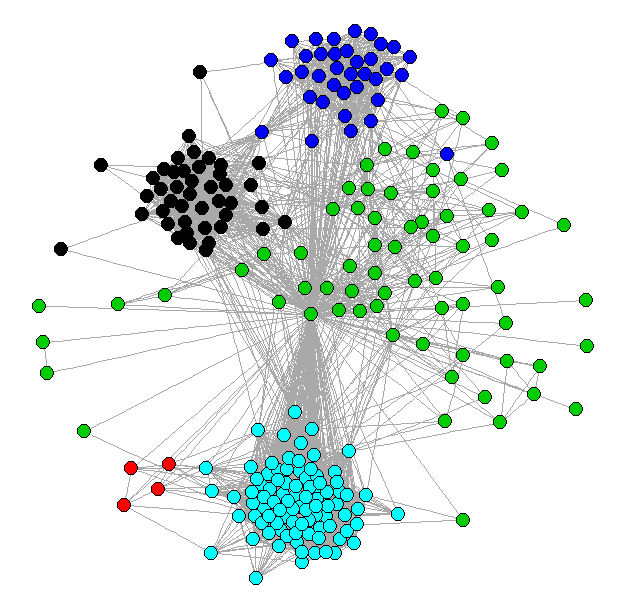
\includegraphics[width= 0.6\textwidth]{figure/lp.png}\\
  \caption{社区发现算法的结果,不同颜色代表不同的社区ID}
   \label{fig:mlp_cd}
\end{figure}

\iffalse
文献\cite{raghavan2007near}给出了一种基于标签传播(Label Propogation,LP)来解决社区发现问题的算法。
LP算法的思想非常简单:最初的时候我们为图中每个顶点分配一个单独的社区ID,
然后我们迭代式地为每个顶点更新社区ID。
每次迭代每个顶点将其邻居顶点所属社区ID出现次数最多的那个作为自己新的ID。
当$G$中每个顶点的社区ID基本上不再变动时,算法结束。
与其他图塌缩方法(例如最大匹配)相比,基于社区检测的方法能够更好地感知原图中的语义。
上述社区发现过程中,确定每个顶点所属的社区ID并没有使用$G$中任何的先验信息或者是既定的目标函数,
而只是利用了图中顶点与其邻居顶点的局部相似性原理。
\fi
本文借鉴了文献\cite{newman2006modularity}中模块度(modularity)最大化的思想,它是常见的社区检测方法之一。
模块度是常用的一种衡量网络中社区稳定度的方法。
简而言之,对于一个已经分配好社区(或划分)的图,分配在同一社区的边占总边数的比例,与对这些边随机分配得到的概率期望,这两者的差就是其模块度。
图\ref{fig:modu_paritition}比较了一个简单图上的基于最大匹配和模块度优化进行塌缩的结果,从中可以明显看出后者更好地保留了原图中的稠密子结构,
即更好地保留了图中的语义成分。

用数学预言描述,设$d_v$表示顶点$v$的度数, $C_v$表示节点$v$所在社区的ID,图的模块度定义如下:
\begin{equation}
\label{eq:mod}
Q = \frac{1}{2W}\sum\limits_{u, v \in V} \left[w_{u,v} - \frac{{d_u}{d_v}}{2W} \right]\delta \left(C_u, C_v\right),
\end{equation}
其中$\delta(C_u, C_v)$表示顶点$u, v$是否处于一个社区,即如果$C_v = C_u$那么$\delta(C_u, C_v)$等于1;否则为0。
$w_{u,v}$表示边$(u,v)$的权重,对于不带边权的图,可以认为如果$(u,v)\in E$那么$w_{u,v}=1$,
否则为0。$W$表示图中所有边的权重之和,即$W=\sum_{(u,v) \in E}w_{uv}$。
\begin{figure}[t]
    \centering
    %\subfig[fjalkf]
    \begin{subfigure}[b]{0.4\linewidth}        %% or \columnwidth
        \centering
        \label{fig:two:one}
	\resizebox{!}{!}{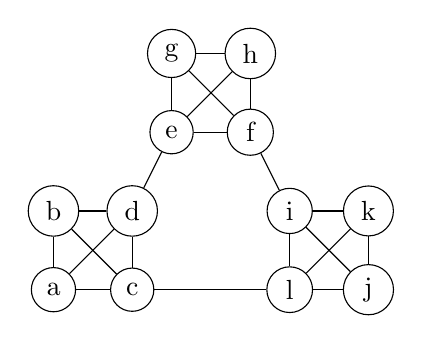
\begin{tikzpicture}
\tikzset{vertex/.style = {shape=circle,draw,minimum size=10 pt}}
\tikzset{edge/.style = {-,> = latex'}}
% vertices
\node[vertex] (a) at  (0,0) {a};
\node[vertex] (b) at  (0,1) {b};
\node[vertex] (c) at  (1,0) {c};
\node[vertex] (d) at  (1,1) {d};

\node[vertex] (i) at  (3,1) {i};
\node[vertex] (j) at  (4,0) {j};
\node[vertex] (k) at  (4,1) {k};
\node[vertex] (l) at  (3,0) {l};

\node[vertex] (e) at  (1.5,2) {e};
\node[vertex] (f) at  (2.5,2) {f};
\node[vertex] (g) at  (1.5,3) {g};
\node[vertex] (h) at  (2.5,3) {h};
%edges
\draw[edge] (b) to (a);
\draw[edge] (b) to (c);
\draw[edge] (a) to (d);
\draw[edge] (b) to (d);
\draw[edge] (c) to (a);
\draw[edge] (c) to (d);

\draw[edge] (e) to (h);
\draw[edge] (e) to (f);
\draw[edge] (e) to (g);
\draw[edge] (f) to (h);
\draw[edge] (f) to (g);
\draw[edge] (g) to (h);

\draw[edge] (i) to (l);
\draw[edge] (i) to (k);
\draw[edge] (i) to (j);
\draw[edge] (l) to (k);
\draw[edge] (l) to (j);
\draw[edge] (j) to (k);


\draw[edge] (f) to (i);
\draw[edge] (d) to (e);
\draw[edge] (c) to (l);
\end{tikzpicture}
}
	\caption{$G$}
	\label{fig:figure2:figure1} 
	\end{subfigure}
    \begin{subfigure}[b]{0.4\linewidth}        %% or \columnwidth
     \centering
	\resizebox{!}{!}{\input{temp7.tikz}}
	\caption{通过最大匹配塌缩后的图$G\prime$}
	\label{fig:figure2:figure2}
    \end{subfigure}
    \begin{subfigure}[b]{0.4\linewidth}        %% or \columnwidth
     \centering
	\resizebox{!}{!}{\input{temp6.tikz}}
	\caption{通过模块度优化塌缩后的图$G\prime$}
	\label{fig:figure2:figure2}
    \end{subfigure}
    \caption{(a)为一个简单的示例图$G$,(b)为$G$该通过最大匹配算法塌缩后形成的图$G\prime$, 每个顶点代表$G$中的一个划分,(c)为$G$通过模块度优化算法塌缩后形成的图$G\prime$, 每个顶点代表$G$中的一个划分}
    \label{fig:modu_paritition}
\end{figure}
这个定义表面模块度是一个取值在-1与1之间的标量,并且模块度越大,其社区划分的质量越高。
按照上面的定义,我们有如下的推论:
\theorem{根据上面的定义,我们实际上可以得到模块度$Q$定义的简单形式:
\begin{equation}
Q = \sum\limits_{c \in P} \left[\frac{I_c}{2W} - {\left(\frac{S_c}{2W}\right)}^2 \right]
\end{equation}
}
其中,$I_c$表示ID为$c$的社区中两个端点都在$c$中的边的权重之和,而$S_c$表示社区$c$中所有顶点的度数之和,
即$S_c = \sum_{v \in V} {d_v}$
\begin{proof}
根据\label{eq:modularity}的定义,如果顶点$u, v$属于不同社区的话,那么显然有$\delta(C_u, C_v)=0$,
因此只要考虑属于同一社区的点对,即我们可以把公式\ref{eq:mod}改写为:
\begin{equation}
\begin{aligned}
Q &= \frac{1}{2W}\sum\limits_{u, v \in V} \left[w_{uv} - \frac{{d_u}{d_v}}{2W} \right]\delta(C_u, C_v) \\
& = \frac{1}{2W}\sum\limits_{c \in P} {\sum\limits_{u, v \in c} { \left[w_{uv} - \frac{{d_u}{d_v}}{2W} \right]}} \\
& = \frac{1}{2W}\sum\limits_{c \in P} \left[{\sum\limits_{u, v \in c} { w_{uv} - \frac{\sum\nolimits_{u,v \in c}{{d_u}{d_v}}}{2W}}}\right] 
\end{aligned}
\end{equation}
注意到有$I_c=\sum\nolimits_{u, v \in c}  w_{uv}$, 
并且有$\sum\nolimits_{u,v \in c}{{d_u}{d_v}} =
\sum\nolimits_{u \in c}{d_u} \sum\nolimits_{v \in c}{d_v} = S_c S_c = {S^2_c}$。
因此,我们有如下的定理:
\begin{equation}
\begin{aligned}
Q &= \frac{1}{2W}\sum\limits_{c \in C} \left[I_c - \frac{S_c^2}{2W} \right] \\
& = \sum\limits_{c \in P} \left[\frac{I_c}{2W} - {\left(\frac{S_c}{2W}\right)}^2 \right]
\end{aligned}
\end{equation}
\end{proof}

我们下面给出基于模块度优化的图划分方法。
迭代初始化时每个顶点拥有一个单独的ID,考虑把某个顶点$u$重新放入到某个新的分块$C$后,整个图$G$的模量会发生变化,
我们用符号$\Delta Q_{u,C}$表示。
根据模量的定义,我们有:
\begin{equation}
\begin{aligned}
 \Delta Q_{u,C}=\left[ \frac{I_c+w_{u,C}}{2W} - {\left(\frac{S_C + d_u}{2W} \right)}^2 \right] -
 \left[ \frac{I_C}{2W} - {\left(\frac{S_C}{2W} \right)}^2 \right] - {\left(\frac{d_u}{2W}\right)}^2 
\end{aligned}
\end{equation}
其中,$w_{u,C}$指的是顶点$u$指向分块$C$的所有的边的权重之和。经过若干步骤的化简,最终我们可以得到模块度变化的简单形式:
\begin{equation}
\begin{aligned}
\label{eq:deltaQ}
 \Delta Q_{u,C}=\frac{w_{u,C}}{2W} - \frac{S_Cd_u}{2W^2} 
\end{aligned}
\end{equation}
上式告诉我们,将某个顶点从之前的分块移除并重新放入新的分块之中时,只需考虑图中的局部信息就可以计算出模块度的变化量,
而不需要按照式\ref{eq:mod}那样暴力遍历所有边。

因为Spark平台内部RDD的计算无法按照异步(asynchronize)方式生成,
Spark需要严格同步(synchronize)本轮迭代中所有线程的计算结果,才会进入下一步的迭代。
所以在第$t$轮迭代中计算维护图中顶点的相关信息只能基于第$t-1$轮迭代各顶点已有的信息。
基于这个特性,我们对图进行基于模块度优化的塌缩算法如\ref{alg:mlgp}所示。
算法包含三个参数,$\alpha, \beta, k$。
其中,$\alpha$指的是反复塌缩过程的目标划分数目,如果迭代过程中当前的划分数目大于$\alpha$,就继续迭代下去。
$\alpha$取值的具体设定与第二步中单节点图划分算法可以处理的输入图规模有关。
$\beta$指的是我们的塌缩方法(即基于模块度进行社区检测)的迭代次数。
参数$bs$代表图划分过程中每个分块可以包含顶点数目的上限。
如果$bs$设置得较大,那么最终每个分块规模会比较小,而分块数目较多;
如果$bs$设置得较小,那么每个分块规模可能较大,而分块数目较少。
首先初始时赋予图中每个顶点一个不同的ID(第2行)。
算法会一直迭代直到当前图的顶点数目小于$\alpha$(第3行),每次迭代过程中都会更新划分$P$并生成新的塌缩图(第17-18行)。
每次的迭代内部包含一个迭代$\beta$次的社区发现过程(第4-16行)。
如果模块度有增益,那么一个顶点会移入到其邻居顶点所属的社区中(第7-16行)。
注意到如果待加入的那个社区中包含的顶点权重之和(根据公式\ref{eq:vertex_weight},权重之和表示该社区在原输入图$G_0$对应的划分中的顶点数目)
已经超出了分块阈值$bs$,那么该社区不会接受新的顶点加入(第9行)。
这保证了最终分块的负载均衡,即每一个分块的顶点数目都不会超过$bs$。

%\begin{figure}[tbp]
\begin{algorithm}[h]
\captionof{algorithm}{Modularity-based Graph Coarsening}
\label{alg:mlgp}
\begin{algorithmic}[1]
\Procedure{GraphCoarsening}{$G, \alpha, \beta, bs$}
  %\State {Set block size threshold $bs \gets |V|/k$};
  \State Initialize partition $P$, which assigns each vertex a unique partition ID;
      \While{$|V| \ge \alpha$} \Comment{\#Paritions greater than  $\alpha$}
	  \State $W \gets \sum\nolimits_{u,v \in V} w_{u,v}$; 
	  \For{$i=1$ to $\beta$}
	    \For { $u \in V$}
		\State{$maxGain \gets -1$};
		\For{ $v \in Nei_u$}  \Comment{Loop $u$' neighbors}
		  \If {$|C_v| \ge bs$} \Comment{Partitions with size smaller than $bs$}
		     \State $\Delta Q_{u,C_{v}} \gets \frac{w_{u,C_v}}{2W} - \frac{S_{C_v}d_u}{2W^2}$;
		     \If {$\Delta Q_{u,C_{v}} > maxGain$}
		      \State $maxGain \gets \Delta Q_{u,C_{v}}$
		      \State $newPartition \gets v$
		     \EndIf
		   \EndIf
		\EndFor
		\If {$maxGain > 0$}
		    \State $C_{newPartition} \gets C_{newPartition}\cup\{u\}$;
		    \State $C_{u} \gets C_{u} - \{u\}$;
		    
		\EndIf	
	    \EndFor
	  \EndFor
	  \State update $P$
	  \State {$G \gets $ the coarse-grained graph constructed from $P$}
	\EndWhile
\State \textbf{return} $G$.
\EndProcedure
\end{algorithmic}
\end{algorithm}
%\end{figure}

\subsection{初始划分与恢复步骤}
经过反复塌缩后,原图$G_0(V_0,E_0)$变成了规模足够小的图$G_t(V_t,E_t)$,其中$|V_t| < \alpha$。
此时$G_t$中每个顶点$u$都对应原图$G_0$中的若干紧密连接的顶点集合$C_u$,$u$的权重对应$|C_u|$;
$G_t$中的每条边$(u,v)$都对应$G_0$中横跨集合$C_u$与$C_v$之间的边,$(u,v)$的权重对应边割集中边的数目。
因此,对$G_t$的划分$P_t$可以一一对应到对$G_0$的划分$P^\star$。
并且,顶点$u \in V_t$是$P_t$的最小划分单元,而对应到$G_0$中,集合$C_u$才是$P^\star$的最小划分单位。
$C_u$中的顶点是不可重新进行划分的,因为它们的分块在之前的塌缩过程中就已经由基于模块度的社区发现逻辑决定了。

我们直接使用METIS软件包提供的单节点算法求解$G_t$的划分$P_t$。
具体求解时,仍然按照之前的目标:即顶点数目的划分均衡以及边割权重的最小化。
因为METIS只能处理规模较小的图,所以$\alpha$的值应当设置在合理的范围内。

恢复过程比较简单,对$P_t$中的每个顶点$u$,直接把其在$G_0$中一一对应的顶点集合$C_u$中的所有顶点的分块号,
设置为$u$在$P_t$中的分块号即可。

\iffalse
\begin{algorithm}[H]
\captionof{algorithm}{Multi-Level Graph Partitioning}
\label{alg:mlgp}
\begin{algorithmic}[1]
\Procedure{MultiLevelGraphPartition}{$G, \alpha, \beta, k$}
	\While{\#partitions $\ge \alpha$}
		\State $P \gets $ results of modularity-based community detection for $\beta$ iterations;
		\State Construct $G\prime$ from $P$; \Comment{Coarsen.}
	\EndWhile  
	\State $P_1 \gets $ Run local graph partitioning on $G\prime$. \Comment{Final refinement.}
	\State restore partition $P\prime$ from $P_1$ \Comment{Project back to the orignal graph.}
\EndProcedure
\end{algorithmic}
\end{algorithm}
\fi
\section{基于Spark平台的算法的实现}
我们基于Spark提供的分布式图计算框架GraphX来实现算法的逻辑。
首先给出顶点的定义,如图\ref{fig:node_struct}所示。
可以看到,Node这个结构记录了顶点的ID、所属分块ID、权重、顶点到所属分区的连接数、顶点到邻居分区的连接数等信息。
这些信息在计算过程中会不断的在顶点之间传输、交换、维护。
\begin{figure}[h]
  \centering
\begin{lstlisting}
class Node extends Serializable{
    val vID:Long
    val pID:Long
    var weight:Double = 1.0,
    var pWeightSum:Double = 0.0,
    var nbrPWeightSum:Double = 0.0
    var modularity:Double
    ...
}
\end{lstlisting}
  \caption{Node结构体}
   \label{fig:node_struct}
\end{figure}
\subsection{塌缩过程}
迭代的总流程分为两个阶段,具体如图\ref{fig:coarse}所示。
在Map阶段,所有顶点向其邻居顶点发送描述自己本身信息的消息,
这些消息结构中包含(srcID, dstID);在Reduce阶段(第3行),发送至同一目的地的若干消息被组装为一个消息列表,
目标顶点收到这些消息后,在本地进行必要的计算获得周围顶点的全部信息,然后就可以根据公式\ref{eq:deltaQ}计算出$\Delta Q$的大小。
根据计算出来的模块度增量,顶点更新自己所属的分块(第4行)。
当$\beta$次迭代过程结束后,开始一次塌缩过程(第9行)。
\begin{figure}[H]
  \centering
\begin{lstlisting}
var graph = Graph(vertexRDD, edgeRDD)
for (iter <- 1 to beta) {
    var newVertexRDD = graph.aggregateMessages()
    Graph = Graph(newVertexRDD, graph.edges)
    // ...
    //send info to neighbors  
}
var edges = generateEdges(graph)
graph = Graph(newVertexRDD, edges)
\end{lstlisting}
\caption{一次塌缩过程}
   \label{fig:coarse}
\end{figure}

其中,generateEdges方法具体描述了塌缩过后重新生成规模更小的图的过程,具体细节如图\ref{fig:smaller_graph}所示。
\begin{figure}[t]
  \centering
\begin{lstlisting}
graph.triplets.map{
  t => Edge(t.srcAttr.pID, t.dstAttr.pID, t.attr)
	.flatMap {
	    e => {
	      ...
	      List()
	    }
	}.reduceByKey()
	 .map{
	    e => Edge(new Node(), new Node()) //construct new edge
	    }
}
\end{lstlisting}
\caption{由中间划分生成更小的图}
   \label{fig:smaller_graph}
\end{figure}
首先统计有哪些边在当前图中横跨了不同的分块(第2-7行),然后使用reduceByKey操作把这些边变成一条新的边(第8-9行),
这个过程中边的数量得到减少,并且新边拥有新的权重,以及两边端点的新权重。
\subsection{初始划分与恢复过程}
为了能够将原始图的划分恢复出来,塌缩过程中每生成一个规模更小的图$G_i \rightarrow G_{i+1}$,
我们都单独使用一个RDD以KV对的方式记录$V_i$与$V_{i+1}$中顶点的对应关系,其中$key$是
$V_i$中顶点的ID,$value$是该顶点在$V_i$中的分块ID,同时也是$V_{i+1}$中的某个顶点ID。
这样如果迭代了$t$次就有$t$个单独的$RDD_{1}, RDD_{2}, \dots, RDD_{t}$。
当图的规模达到可以接受的范围之后,我们使用collect操作将其收集到Driver Program,使用单节点算法直接对其划分。
然后再使用parallelize方法将划分结果重新变成一个元素类型为(vertexID, partitionID)的RDD数据,记其为$RDD_{t+1}$。
恢复过程的具体细节如图\ref{fig:restore}所示。
对$t+1$个$RDD$,我们取最后一个$RDD_{t+1}$(第1行),将它与互换过KV(即由原来的$(key,value) \rightarrow (value, key)$,第3行)的$RDD_{t-1}$做join操作得到$V_t$与$V_{t-1}$中顶点的对应关系(第4行),
再与交换过KV的$RDD_{t-2}$做join操作就得到$V_t$与$V_{t-2}$中顶点的对应关系,如此循环下去,直到得到$V_t$与$V_0$中顶点的对应关系。
最后对生成的$resultVertexRDD$中元素进行互换(第6行),这样该RDD元素的点对就变成了(vertexID, partitionID)的格式,即得到了原图上的划分。
\begin{figure}[h]
  \centering
\begin{lstlisting}
var resultVertexRDD = rdds.last
for (i <- (1 until rdds.length).reverse) {
    coarsen_before = rdds(i-1).map(e => 
			  (e._2, e._1)) //swap key-value
    resultVertexRDD = resultVertexRDD.join(coarsen_before).map(...) 
}
//swap key-value
resultVertexRDD = resultVertexRDD.map(e => (e._2, e._1)) 
}
\end{lstlisting}
\caption{恢复过程}
   \label{fig:restore}
\end{figure}
\section{实验评估}
\subsection{实验环境及数据集}
我们采用的实验环境与上一章节完全一样。
在数据集方面,我们一共使用了三个真实的数据集。
其中,wiki-talk记录了维基百科用户共同编辑条目的关系;
cit-Patents记录了1963至1999年间美国所有记录在案的专利之间的互相引用情况;
ljournal-2008记录了一个虚拟社交网络中所有用户的交友关系。
每个图数据一开始为普通的文本格式,每一行代表图中的一条边。
在开始实验前,所有的数据集都预先上传到分布式文件系统HDFS上。
\begin{table}[h]
\caption{数据集描述}
\label{tab:dataset2}
\centering
\begin{tabular}{|l|r|r|r|r|}
\hline
\textbf{数据集} & \textbf{顶点数} & \textbf{边数} & \textbf{顶点平均度数} & \textbf{大小} \\
\hline
wiki-talk     \footnotemark[1]       & \num{2394385} & \num{5021410}          &\num{2.10}                   & 66.5MB\\
\hline
cit-Patents      \footnotemark[2]     & \num{3774768}  & \num{16518948 }          & \num{4.38}             & 203.4MB\\
\hline
ljournal-2008  \footnotemark[3] & \num{5363260} & \num{79023142}         & \num{14.73}            &1.2GB\\
\hline
%arabic-2005 \footnotemark[5]   & \num{22744080} & \num{639999458}      & 28.14           & 10.9GB\\
%\hline
%twitter-2010    & \num{41652230 } & \num{1468365182} & 26.1GB\\
%\hline
\end{tabular}
\end{table}
\footnotetext[1]{https://snap.stanford.edu/data/wiki-Talk.html}
\footnotetext[2]{https://snap.stanford.edu/data/cit-Patents.html}
\footnotetext[3]{http://law.di.unimi.it/webdata/ljournal-2008/}
%\footnotetext[5]{http://law.di.unimi.it/webdata/arabic-2005/}
\subsection{算法的有效性}
我们主要从划分结果的边割大小衡量算法的划分质量。
图 \ref{fig:partitionquality} 展示了我们的算法mod\string_MLP与其它相关算法的最终划分质量比较。
其中,METIS\cite{Karypis95metis}是经典的、久经改良的单节点图划分方法;
lp\string_MLP\cite{DBLP:conf/icde/WangXSW14}也是一种多层次划分方法,但是其塌缩步骤基于标签传播\cite{raghavan2007near}(Label Propogation,LP)算法实现;
Random指对图中顶点采取随机方式直接等概率分配分块ID。
具体运行时,上述四种算法的分块目标数被设为一样的数值$\alpha=300$,内部循环深度$\beta=5$,等到每个算法完全运行结束后再基于划分结果计算边割的大小。
METIS方法运行在一个拥有64G物理内存的计算节点上,
而mod\string_MLP以及lp\string_MLP都被实现为基于Spark的分布式算法。
\begin{figure}[h]
  \centering
  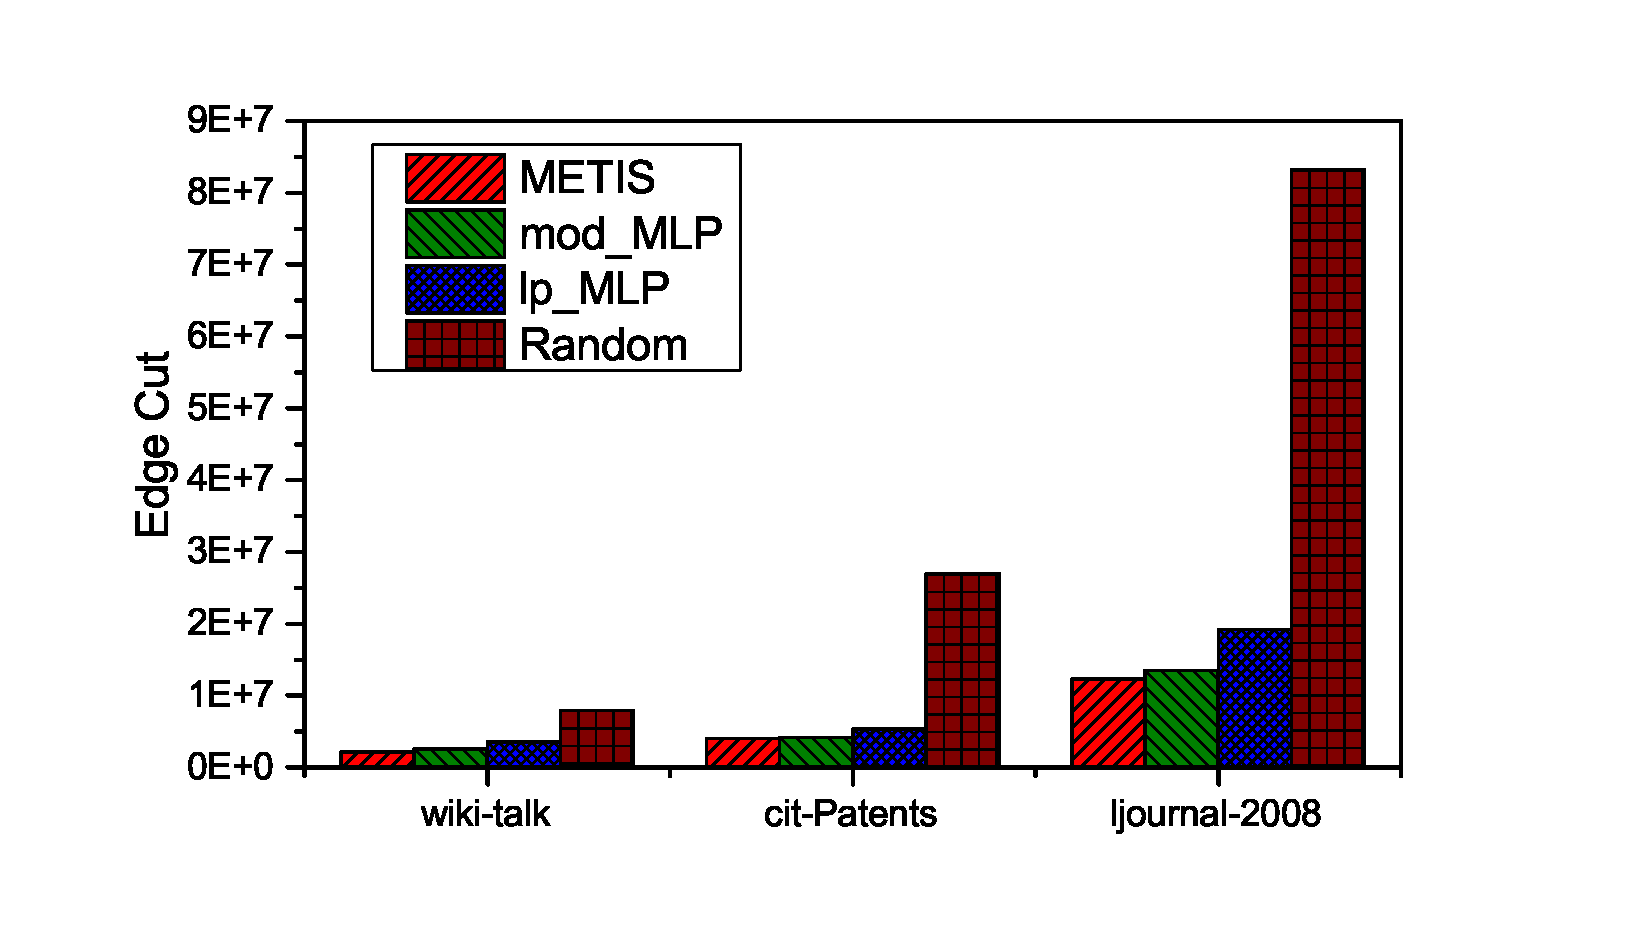
\includegraphics[width= 1\textwidth]{figure/p_quality.eps}\\
  \caption{划分质量对比}
   \label{fig:partitionquality}
\end{figure}

从图中可以看出,其余三种算法的划分质量都大大超过了随机划分。
在三个数据集上,mod\string_MLP都表现出了可以与METIS相媲美的效果。
同时可以看到mod\string_MLP的划分边割比lp\string_MLP要小,并且随着图规模的变大改进越明显。
这表明相比于标签传播仅仅利用了顶点之间的局部相似性,基于模块度最大化的塌缩过程使用了全局的模块度信息,
使得社区划分过程更好地向最优化方向前进,从而更好地保留了原图中稠密的子结构。
\subsection{算法的计算效率}
图\ref{fig:block_with_time}展示了在wiki-talk数据集上,mod\string_MLP运行过程中塌缩图$G_i$的顶点数目与运行时间的变化关系。
运行过程中我们不设置算法的目标分块数,试图让算法“自由”地运行下去。
从图中可以看出,分块数自然而然地随着计算过程的深入而逐渐减少。

图\ref{fig:partition_time}比较了METIS、lp\string_MLP和mod\string_MLP在三个数据集上的运行时间。
具体运行时,上述四种算法的目标分块数被设为一样的数值$\alpha=300$,等到每个算法完全运行结束后再统计各自的运行时间。
从图中可以看到两个分布式算法的计算效率都远远超过了单节点算法METIS。
另一方面,在所有数据集上mod\string_MLP都比lp\string_MLP提前了大约$20\%$到$27\%$的时间完成计算任务。
如果我们单纯考虑两者塌缩过程的区别,显然理论上lp\string_MLP算法中基于标签传播LP算法的单次迭代过程
是略微快于mod\string_MLP算法中基于模块度优化的单次塌缩过程的,
因为后者每个顶点需要从邻居顶点收集相关信息计算模块度的变化$\Delta Q$,而前者只要简单选择邻点所属的社区ID出现次数最多的那个即可。
但是基于模块度优化的过程比LP有更好的划分质量,因此如果从算法整体考虑,前者所需的迭代次数小于后者,从而减少了计算时间。
实验中,我们都设置塌缩过程中的内部迭代次数$\beta=5$,结果发现lp\string_MLP的总迭代次数超过mod\string_MLP的所需迭代次数的$20\%$左右。
这与图\ref{fig:partition_time}中算法的总体运行时间表现一致。

\begin{figure*}[t]
\centering
\begin{subfigure}[b]{0.48\textwidth}
	\center
	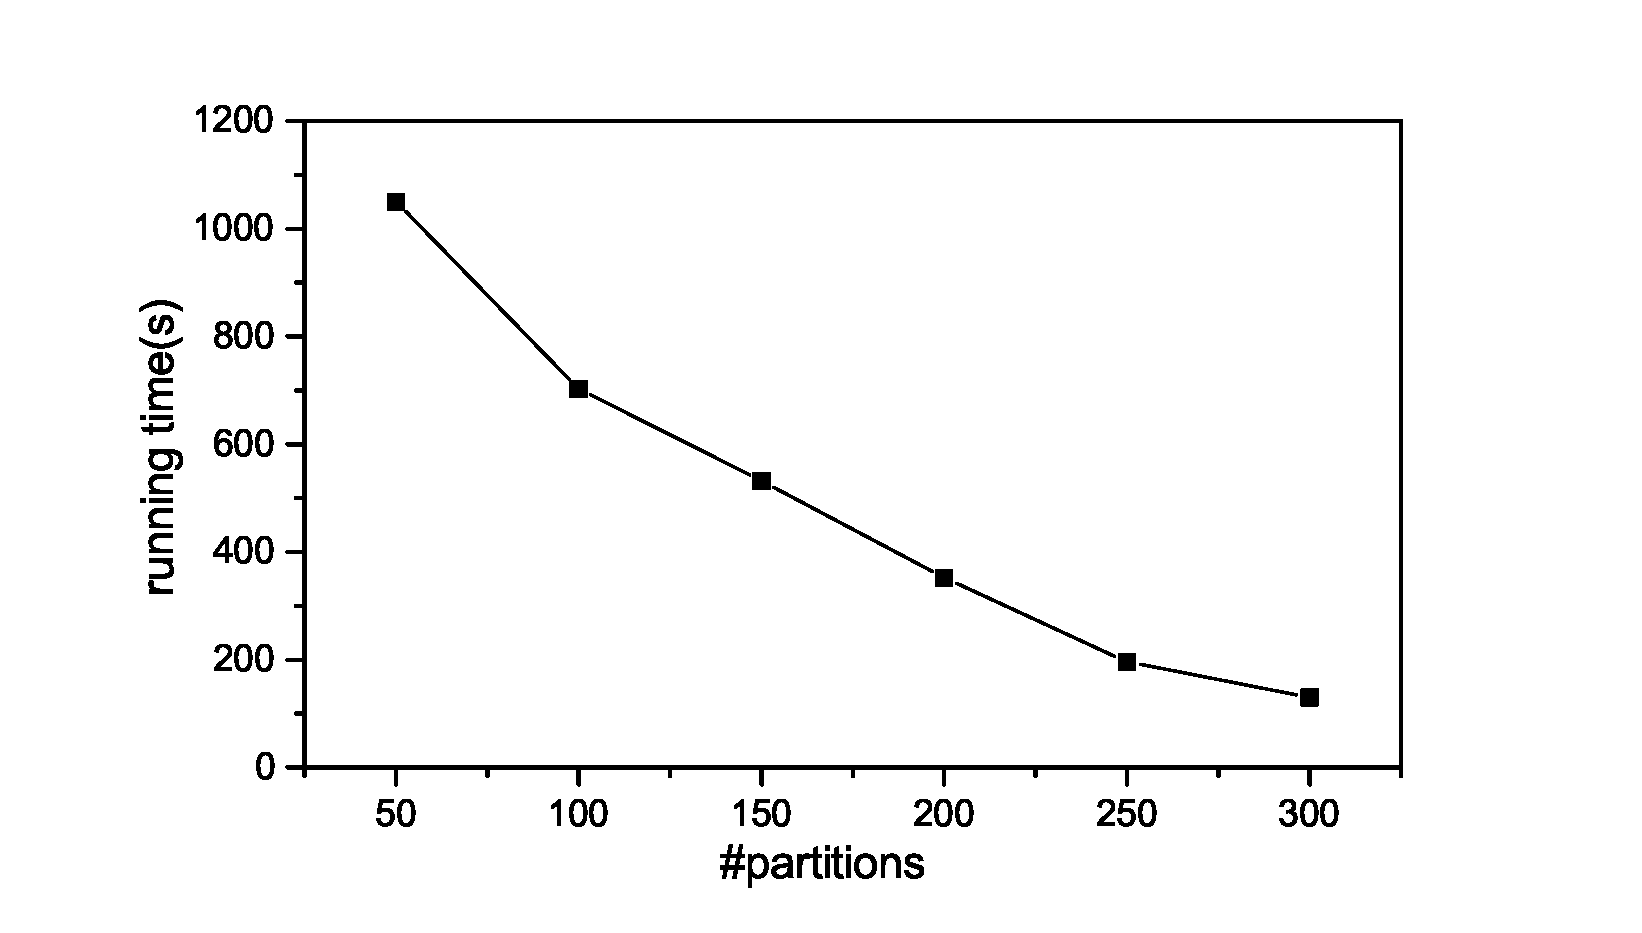
\includegraphics[width=1\textwidth]{figure/block_time.eps}
	\caption{wiki-talk上分块数与时间的变化关系}
	\label{fig:block_with_time}
\end{subfigure}
\begin{subfigure}[b]{0.48\textwidth}
	\centering
	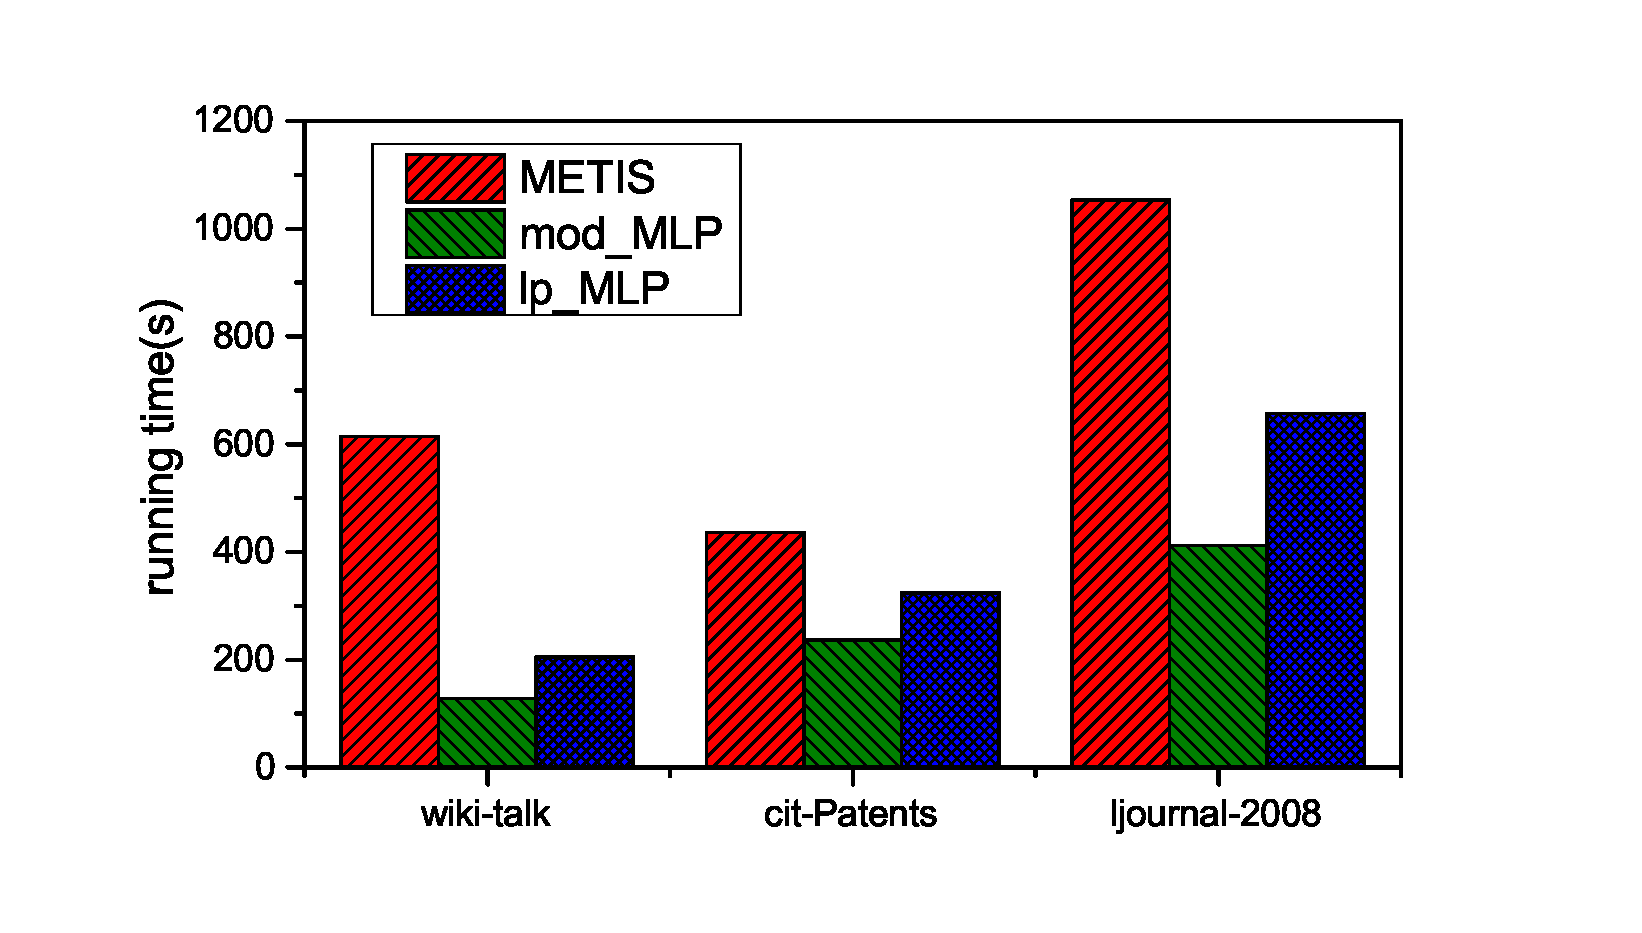
\includegraphics[width=1\textwidth]{figure/running_ti.eps}
	\caption{算法的运行时间比较}
	\label{fig:partition_time}
\end{subfigure}
\label{fig:running_cond}
\caption{左图为wiki-talk数据集上随着算法的运行分块数的变化情况;右图为不同算法在数据集上的运行时间比较}
\end{figure*}

\begin{figure}[h]
  \centering
  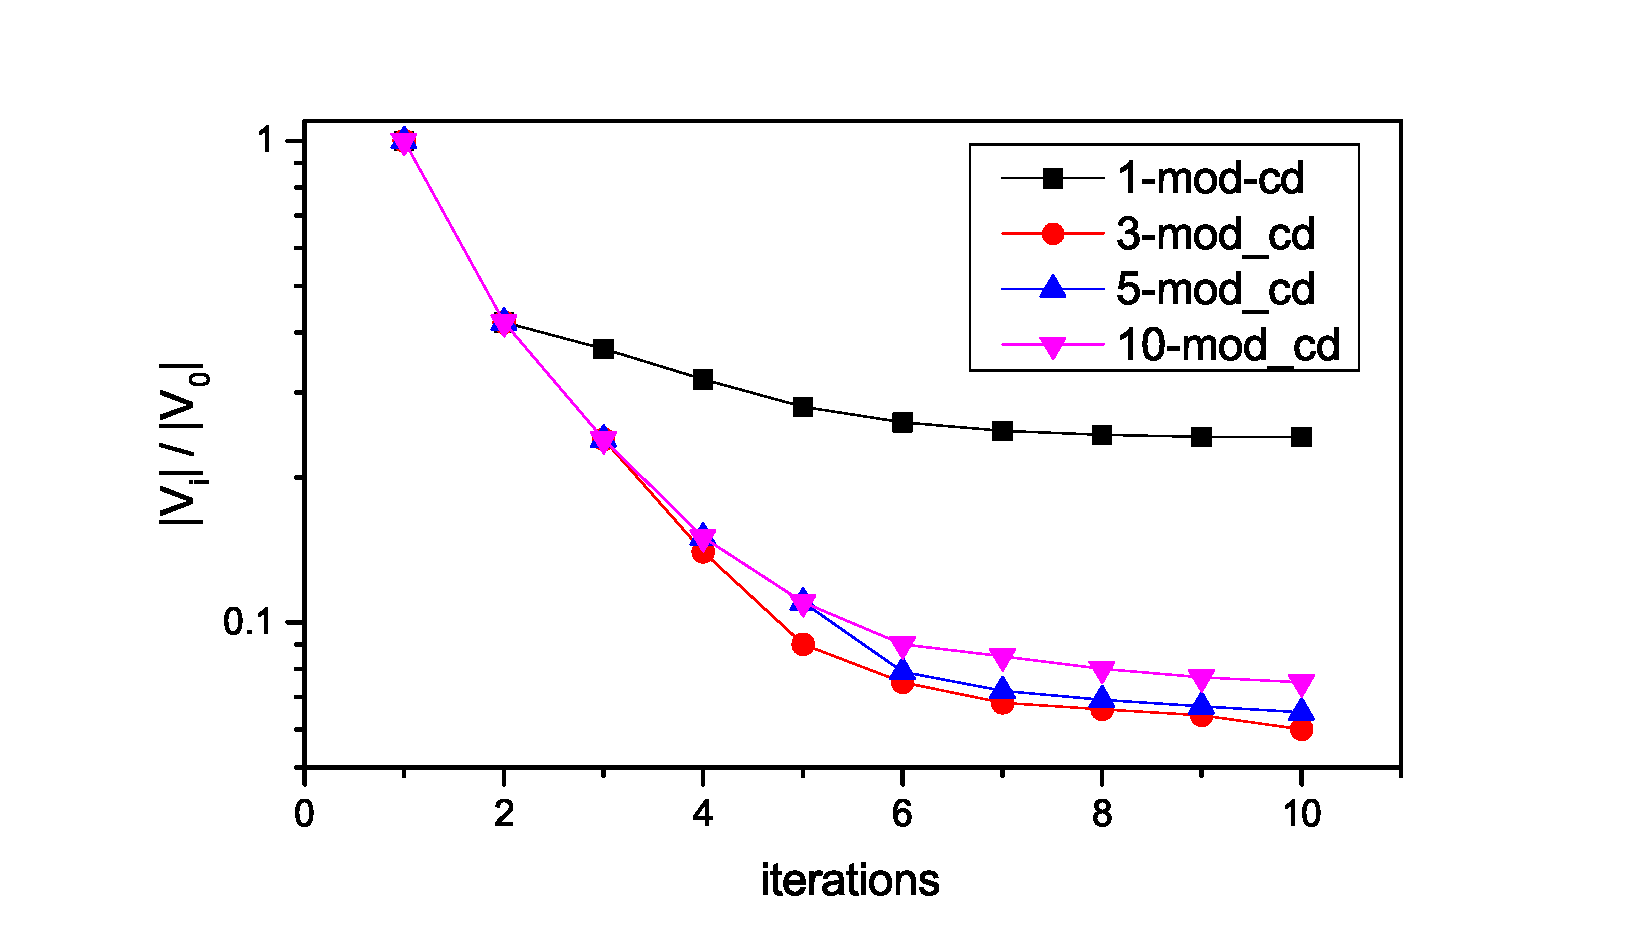
\includegraphics[width= 1\textwidth]{figure/conv_time.eps}\\
  \caption{参数$\beta$与运行过程中中间分块数目的关系}
   \label{fig:conv_time}
\end{figure}

图\ref{fig:conv_time}展示了参数$\beta$与mod\string_MLP塌缩过程中中间分块数目变化的关系。
注意到这里的分块数指的是内部迭代过程中社区发现算法所看到的社区数量。
我们设置$\beta$的值分别为1,3,5,10,例如图例“1-mod-cd”表示塌缩过程中采用内部迭代深度为1的基于Modularity的Community Detection算法,
并观察总共10次迭代过程(指内部迭代次数)以内分块数与$|V_0|$比例的变化。
从图中可以看出,当$\beta=10$时总的迭代次数为$1\times 10$,此时算法退化成一个社区发现过程;
当$\beta=1$时算法总的迭代次数为$10\times 1$,算法总共进行了10次塌缩过程,但是每次塌缩对图的规模改变极小。
$\beta=3$与$\beta=5$时的曲线较为类似,并且可以发现每隔$\beta$轮迭代后中间分块数相比于之前有更加明显的下降过程。
这是因为分块数的下降是由两个因素造成:$\beta$轮内部迭代中主要驱动因素是基于模块度最大化的社区发现,
而$\beta$轮迭代之后会刚好有一次塌缩步骤直接降低了图的规模。

\subsection{算法的可扩展性}
\begin{figure}[t]
\centering
\begin{subfigure}[b]{0.48\textwidth}
	\center
	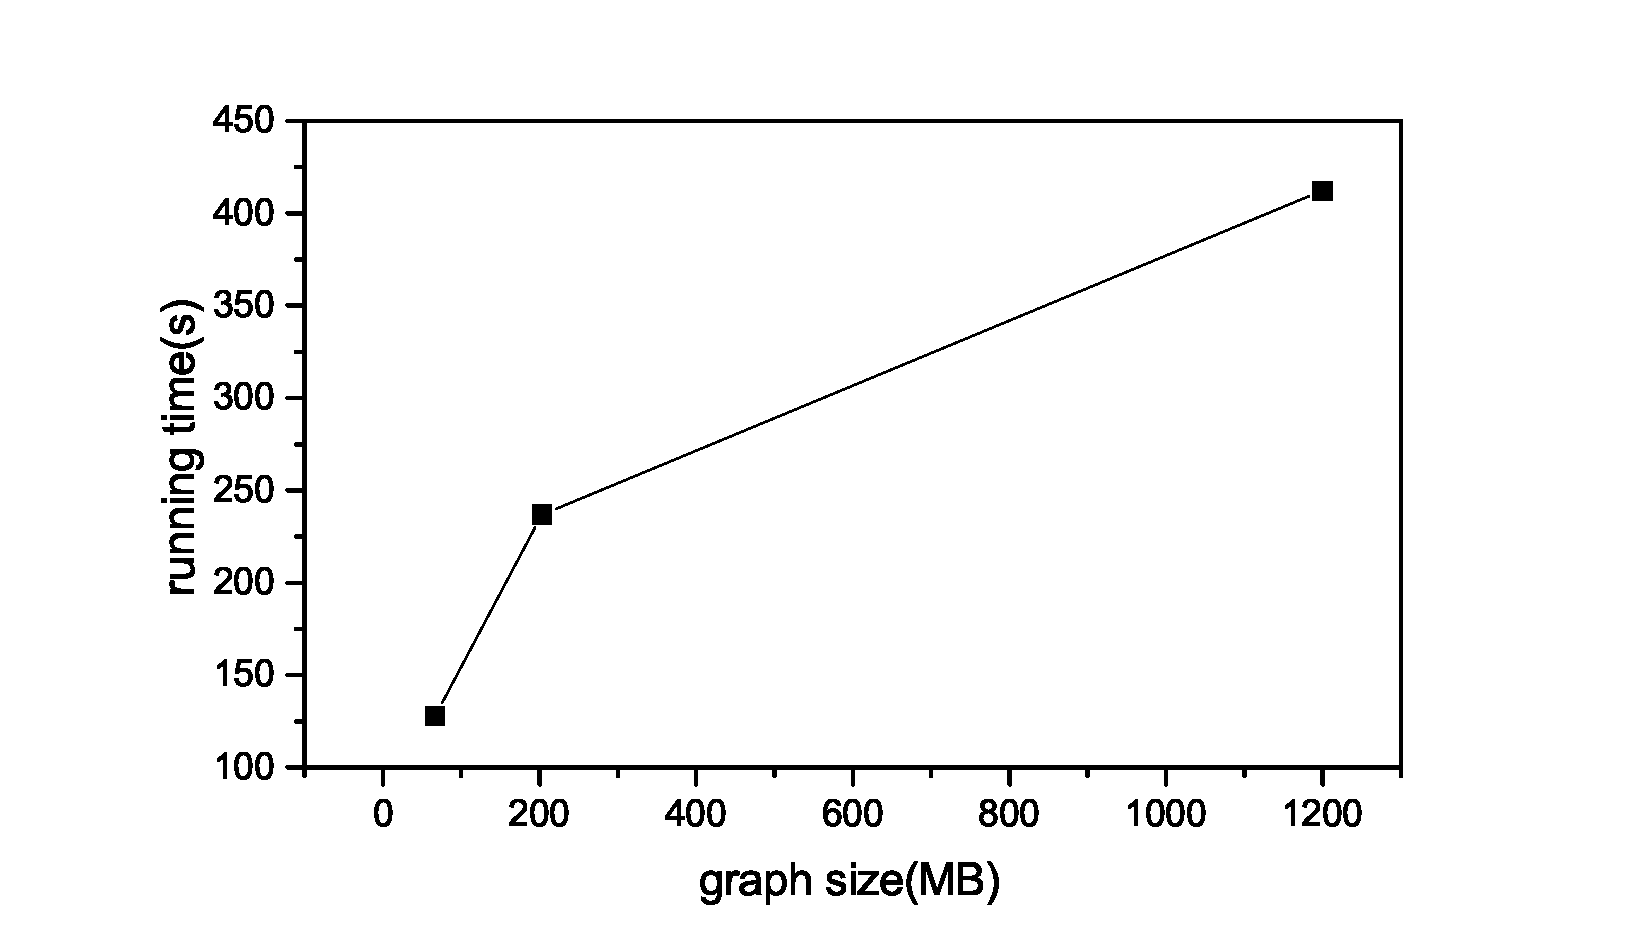
\includegraphics[width=1\textwidth]{figure/data_scala.eps}
	\caption{运行时间与输入图大小的变化关系}
	\label{fig:ch2:data_scalabity}
\end{subfigure}
\begin{subfigure}[b]{0.48\textwidth}
	\centering
	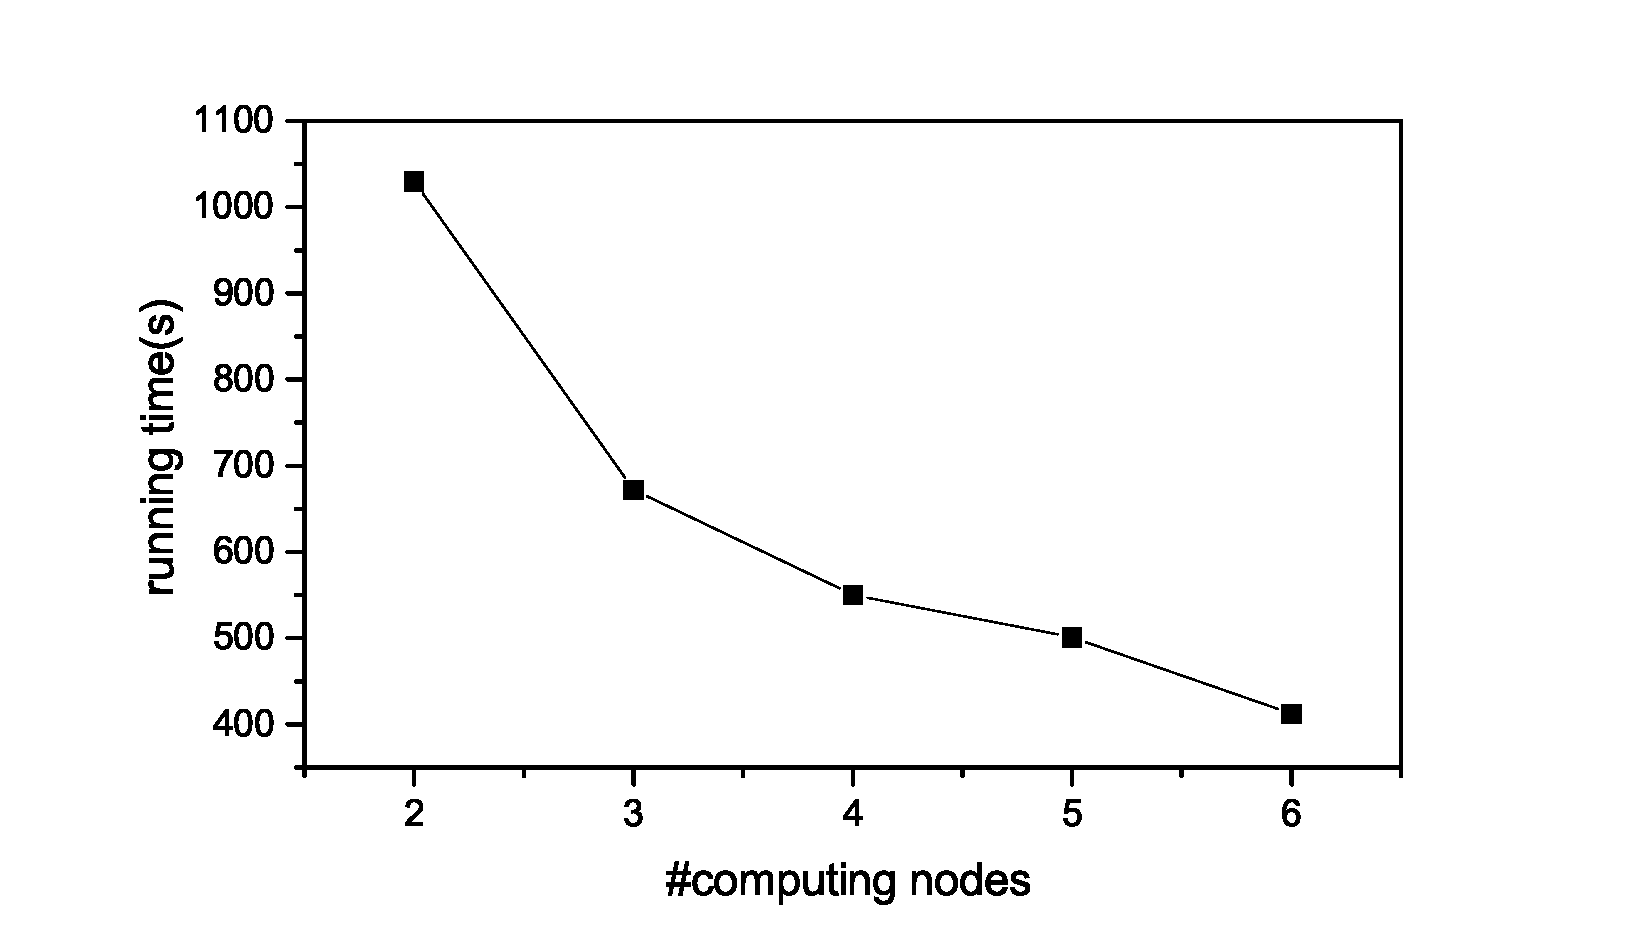
\includegraphics[width=1\textwidth]{figure/node_scalabity.eps}
	\caption{运行时间与计算节点数量的变化关系}
	\label{fig:ch2:node_scalabity}
\end{subfigure}
\caption{算法的可扩展性}
\label{fig:scalabityyy}
\end{figure}
图\ref{fig:scalabityyy}展示了算法的可扩展性。
首先考察算法运行时间随着输入图的规模大小的变化关系,结果如图\ref{fig:ch2:data_scalabity}所示。
图中展示了当集群计算节点数目固定时,对于不同的图数据,运行时间随输入图规模大小变化的情况。 
可以看出,输入图的规模从66MB增长到1.2GB,而对应的运行时间基本上近似地随着输入规模大小线性地变化,
这表明mod\string_MLP具有良好的数据可扩展性。
我们还考察了当输入图的规模固定时,算法运行效率随集群中计算节点数量变化的情况。
输入图为ljournal-2008,固定算法的参数为$\alpha=300$,$\beta=5$,计算节点数量从2增加到6。
实验结果如图\ref{fig:ch2:node_scalabity}所示。
从图中可以看到,对不同规模的输入图,算法的运行时间随集群计算节点的增加而近乎线性地减少,
这表明算法在分布式环境下具有良好的节点可扩展性。

\section{本章小结}
随着现实生活中数据规模的不断扩大,与之对应的图数据规模也不断增加。
普通的单台计算机由于运算内存的限制,远远无法胜任对大规模图数据的计算处理
任务。因此,将图划分成多个子图装载到不同计算节点上中,然后再利用分布式平台
进行后续的计算,是处理大规模图数据唯一可行的方案。

针对大规模图数据的分布式划分问题,本章分析比较了社区发现任务与图划分任务的异同,提出并设计了分布式多层次图划分方法。
算法包括三个典型的步骤:塌缩、初始化分和恢复。
在塌缩过程中,本章借鉴了社区发现的思路,基于模块度最大化进行分块的分配,从而较好地保留了图中的语义信息,即保留了图中的稠密子图结构。
与其它算法相比,本算法有较高的划分质量,同时有较好的可扩展性和计算效率。

%%%%%%%%%%%%%%%%%%%%%%%%%%%%%%%%%%%%%%%%%%%%%%%%%%%%%%%%%%%%%%%%%%%%%%%%%%%%%%%
\chapter{分布式全点对相似度算法}\label{chapter_allSimRank}
\section{概述}
前面章节介绍了计算单源点SimRank相似度的计算方法,如果进一步地考虑计算图$G$中全点对的相似度,
那么不管是直接根据SimRank的定义采用矩阵迭代计算的方法,还是将全点对计算问题简单看做$|V|$个单源点相似度计算问题,
整个计算的开销无疑是不可承受的。
考虑一个现实生活中的拥有数百万节点的大规模图,其邻接矩阵的元素规模达到万亿级别($|V|^2$),
涉及到这么大规模的矩阵乘法需要做复杂的算法设计和程序优化,甚至需要有专门的高性能超算平台来运行相关程序。
如果简单地将全点对相似度计算看做$|V|$个单源点计算问题,那显然没能够充分挖掘出问题内在的可并行性。
因此,需要重新设计高效的算法来计算图$G$中全点对的相似度。
针对此问题,本章采用“分而治之”的思想,将复杂的计算任务分解为规模更小、更容易处理的子任务。
我们首先对原图进行划分,然后计算每个分块内部点对的SimRank相似度;接着将各个分块当做单独的顶点,求取分块之间的相似度。
最后基于这两个中间结果计算出所有点对的全局相似度。
\section{相关工作}
目前学术界对全点对SimRank相似度计算问题的研究,可以概括如下:

\textbf{基于矩阵乘法的计算方法}。 
Jeh和Widom\cite{jeh2002simrank}提出了第一个基于矩阵乘法的SimRank迭代计算方法,它可以计算全点对的相似性,其复杂度为$O(kn^2d^2)$
文献\cite{lizorkin2008accuracy}随后通过剪枝、局部访问等技术在矩阵乘法层面将算法的时间复杂度降低到$O(kn^2d)$。
文献\cite{yu2012space}使用了快速矩阵乘法来加速计算过程。
文献\cite{yu2013towards}进一步将算法的时间复杂度降低到$O(kn^2d^{\prime})$,其中$d^\prime < d$。
文献\cite{li2010fast1}提出了一种基于Kronecker乘积和矩阵奇异值分解(SVD)的非迭代算法,
该算法首先在$O(r^4N^2)$时间内计算出一些辅助矩阵,其中$r$是
输入图的邻接矩阵的秩,然后在$O(r^4N^2)$时间内获取顶点间的的相似度。
文献\cite{he2010parallel}使用了GPU来加速矩阵的计算速度。

\textbf{分布式计算方法}。 文献\cite{DBLP:journals/pvldb/LiFLCCL15}提出了一种并行化蒙特卡罗采样的分布式计算方法,
该方法打破了计算点对相似性之间的递归依赖关系:首先离线计算一个不变矩阵$D$,然后根据$D$在线使用
蒙特卡罗方法快速给出查询。该算法的优点是它是一种通用的方法,可以同时应对单点对、单源点、全点对的相似度计算问题。
然而,$D$的计算被当做一个解线性方程组的过程,这在分布式环境下非常低效,因此虽然算法线上查询的效率很高,
但线下预处理的时间开销非常巨大。它可以处理十亿级别的大规模图,但是在一个拥有10个计算节点且总内存高达3.77TB的集群中,需要大约110小时的预处理时间。
文献\cite{DBLP:conf/bigdata/LiLCD13}提出了基于MapReduce的分布式矩阵乘法。
该算法将其中一个矩阵存放在所有计算节点的内存中,从磁盘中读取另一个按行分割矩阵,将内存中的矩阵与每行做乘法,从而实现了矩阵的分布式计算。
文献\cite{yu2013towards}提出了一种基于增量变化的$DeltaSimRank$算法。该算法发现SimRank可以改写为一种迭代的增量计算方式,
即迭代过程中,不直接计算点对之间的相似度而是计算其相对于上一轮迭代的增量。该方法充分利用了迭代计算过程中很多点对间相似度增量为零的事实,减小了
计算过程中的数据传输量,从而加速了计算效率。

\section{算法的基本框架}
基于第三章中对图做出的划分,我们给出一个计算点对之间近似SimRank相似度的算法。
文献\cite{ilprints579}描述了一种基于图中分块结构(Block Structure)的若干性质来加速计算PageRank的方法,我们的方法直接受到了该算法的启发。
现实生活中的图数据集可以天然划分为若干稠密的分块。从语义层面上讲,这些稠密的分块往往蕴含了最多的人们感兴趣的信息。
本文正是充分利用了这一性质,将相似度分为两个不同的层次:分块之间的相似度以及分块内部点对的相似度,从而提出了一种计算全点对之间近似相似度的算法。
相比原来的SimRank的计算方法,该算法表现除了与其相媲美的有效性,同时极大地提高了计算效率。

假设图已经被划分为若干分块,那么顶点对之间的相似度可以分为两种:
\begin{enumerate}
 \item 位于同一稠密分块之中的顶点对。 在上一章节中,我们已经详细介绍了将原图$G$划分为若干稠密分块的方法,每一个划分好的
 分块都被存放在集群中的某一个计算节点中。 这种情况下可以根据公式\ref{eq:two}直接使用串行计算方法计算出该点对的相似性。
 \item 位于不同分块之中的顶点对。如果分块的大小充分大,那么两个顶点分别处于不同的稠密分块之中意味着较大概率地这两个顶点之间的距离会比较远。
 而回顾随机游走模型,相隔较远的两个随机漫步者通常无法在短距离内(<10)通过游走在某个顶点相遇。
 这表明这两个顶点的相似性会较大概率地在数值上表现得非常小,因此我们直接计算它们的近似相似度。
\end{enumerate}

\subsection{分块间的相似度}
与上一章节类似,假设图中的每一个分块是一个顶点,那么图的划分就形成了一个塌缩图。
基于这个塌缩图,我们首先定义图中边的权重:
\begin{definition}
 塌缩图中边的权重。 假设对图$G$有划分$P=(C_1, C_2, \dots, C_n)$,
 设$L(C_i)$表示分块$C_i$中所有边的数量,包括该分块内部的边以及连接到其它分块的边;
 $L(C_i, C_j)$表示分块$C_i$与分块$C_j$中相连接的边的数量。
 设图$G^\prime$为划分$P$形成的塌缩图,$v_i, v_j \in G^\prime$, 
 且$v_i$为分块$C_i$对应的顶点,$v_j$为分块$C_j$对应的顶点。
 那么定义边$(v_i, v_j)$的权重为:
\begin{equation}
 w(v_i, v_j) = \frac{L(C_i, C_j)}{L(C_i)} 
\end{equation}
$v_i$自己到自己的权重定义为
\begin{equation}
 w(v_i, v_i) = 1-\sum_{v_j \in O(v_i)}{w(v_i, v_j)}
 \end{equation}
显然,一般情况下$w(v_i, v_j)$与$w(v_j, v_i)$是不同的。
\end{definition}
这样经过塌缩后的图$G^\prime$变成了一个加权有向图。
边$(v_i, v_j)$的权重可以粗略理解为某个随机游走者从点$v_i$“逃逸”到点$v_j$的概率。
$w(v_i, v_j)$越大,说明在原图$G$中分块$C_i$与$C_j$的交叉边越多,联系越紧密。

基于以上的定义,我们给出图$G$中各个分块之间的相似度定义:
\begin{definition}
 对原图$G$上的划分$P=(C_1, C_2, \dots, C_n)$,定义分块$(C_i, C_j)$之间的相似度为塌缩图$G^\prime$中顶点$v_i,v_j$之间的相似度。
\end{definition}
 为了将边的权重引入到SimRank模型中,文献\cite{DBLP:journals/pvldb/AntonellisGC08}提出了SimRank++算法。
 算法使用如下的公式计算相似度:
\begin{equation}
  s_{k+1}(u,v) = c \cdot evidence(u,v)  
  \sum_{u^\prime \in I(u), v^\prime \in I(v)} s_{k}(u^\prime, v^\prime)W(u^\prime, u)W(v^\prime, v)
\end{equation}
其中,$c$是衰减系数,并且
\begin{equation}
    evidence(u,v)=\sum_{i=1}^{|I(u)\cap I(v)|}2^{-i} 
   \end{equation}
\begin{equation}
     W(u^\prime, u)=w(u^\prime, u)\cdot \exp(-{Var(\{w(u^\prime,u) \mid u \in O(u^\prime)\}})
\end{equation}

如果写成矩阵的形式,设$V$为evidence矩阵,满足$V(i,j)=evidence(i,j)$,那么整个加权有向图的SimRank相似性度计算过程如算法\ref{algo:wapSimRank}所示。
\begin{algorithm}[h]
\captionof{algorithm}{Weighted All-pair SimRank:wapSimRank}
\label{algo:wapSimRank}
\begin{algorithmic}[1]
\Procedure{WeightedSimRank}{$G^\prime, u, c, k$}
	\State $N \gets |V|$;
	\State $S \gets$ identity matrix $I_N$;
	\For{$ i =1$ to $k$}
		\State $T \gets c\cdot W^T \cdot S \cdot W$;
		\State $S \gets T + I_N -D(diag(T))$; \Comment{$D$ is the diagnal matrix.};
	\EndFor
	\State $S \gets$ element-wise multiplication of $V$ and $S$;
	\State \textbf{return} $S$.
\EndProcedure
\end{algorithmic}
\end{algorithm}
\subsection{点对全局相似度估计}

\begin{definition}
 不同分块间点对的相似度。如果点对$(u,v)$的两个顶点分别属于图的不同分块$C_i$和$C_j$之中,
 并且有分块$C_i$与$C_j$的相似度为$s_{block}(C_i, C_j)$,
 我们使用下式来计算$(u,v)$的其相度:
 \begin{equation}
 \label{eq:avg}
    s(u,v) = s(C_i, u) \cdot s_{block}(C_i, C_j) \cdot s(C_j, v)
   \end{equation}
  其中,$s(C_i, u)$可以看做顶点$u$与其分块的中心点间的相似度,由下式近似给出:
  \begin{equation}
    s(C_i, u) = \frac{1}{|C_i|}\sum_{q \in C_i}{s(u,q)}
   \end{equation}
   即我们使用$u$与其分块内所有顶点的相似度的均值来估计$u$与分块中心的相似度。
\end{definition}
算法\ref{algo:wapSimRank}计算出的分块间的相似度是随着迭代次数收敛的\cite{DBLP:journals/pvldb/AntonellisGC08},
并且分块内点对的SimRank相似度计算过程也是收敛的\cite{jeh2002simrank},
那么由以上式子定义出的分块间点对的相似度也是随着迭代次数收敛的。
因此可以分开计算分块之间的相似度与分块内点对的相似度,
最后再基于它们计算分块间点对的相似度。
综上,我们的算法步骤主要如下:
\begin{enumerate}
 \item 首先根据上一章节描述的方法,对原图$G$做划分,得到若干个分块$P=(C_1, C_2, \dots, C_n)$;
 \item 将各个分块当做一个顶点进行塌缩得到一个加权有向图$G^\prime$,在$G^\prime$运行适用于加权图的SimRank++算法,得到
 分块之间的相似度;
 \item 对所有分块$C_i$直接运行串行的全点对SimRank算法,得到分块内部的顶点对相似度;
 \item 使用公式\ref{eq:avg}计算属于不同分块顶点之间的相似度;
 \item 最后返回全局相似度。
\end{enumerate}
\subsection{算法复杂度分析}
simRank以及其适用于加权图的变种SimRank++的时间复杂度都为$O(kd^2n^2)$。
假设图$G$已经被划分为$m$个分块,则每个分块的顶点数目在$O(n/m)$左右。若
塌缩图$G^\prime$的顶点平均度数为$d_1$,那么第2步的时间复杂度为$O(k{d_1}^2m^2)$。
第3步的时间复杂度为$O(mk{d_2}^2(n/m)^2)$,即$O(k{d_2}^2n^2/m)$,其中$d_2$为每个分块中顶点的平均度数。
第4步计算全局相似度时要考虑所有点对,而根据公式\ref{eq:avg},平摊之后每对顶点对只需常数级别的计算时间,
因此总的时间复杂度为$O(n^2)$。
如果我们考虑主要的计算过程,即第2步和第3步,所需的时间为$O(k{d_1}^2m^2+k{d_2}^2n^2/m)$。
若假设有$d_1=d_2=d$,则时间复杂度为$(kd^2(m^2+n^2/m))$。 
将该复杂度看做变量$m$的函数,则函数在$m=(2n)^{2/3}/2$处有极值,这对我们选择合适的$m$有指导意义。
进一步的,考虑分布式环境下第3步主要由多个计算节点的多个线程同时完成,不妨设总线程数为$T$,
则该函数变为$f(m)=kd^2(m^2+n^2/(Tm)$,其在$m=(n^2/(2T))^{1/3}$处有极值。
对于一个顶点数在$1e6$级别的图来说,如果$T$的规模在$1e2$量级,则计算下来的极值点量级在$1e3$左右。
当然,不同的分块数$m$会影响计算结果的精度,因为分块数越多,意味着由计算得到的近似相似度越多,结果的精度越差。
实际的$m$取值,需要综合考虑各种因素再加以决定。

\section{实验评估}
\subsection{实验环境及数据集}
我们部署的实验环境与上一章节完全一样。
在数据集方面,我们一共使用了4个真实的数据集。
其中三个来自于第二章中实验评估中使用的数据集:eu-2005, ljournal-2008, arabic-2005。
除此之外,我们额外使用了由图wiki-topcats\footnotemark[1]加工而成的小规模图。
wiki-topcats是一个记录维基百科中各个WEB超链接之间引用情况的有向图,
所有的条目都一共被分为17364个不同的类别(category)。
我们挑取其中较大的四个类别(由于wiki-topcats中类别是匿名的,我们暂称它们为C1-C4),
保留类别中的顶点以及它们之间的边,得到了规模如表\ref{tab:dataset3}所示的图。
如无特别说明,下面wiki-topcats特指经我们抽取加工过的图。
\footnotetext[1]{https://snap.stanford.edu/data/wiki-topcats.html}
\begin{table}[h]
\caption{数据集描述}
\label{tab:dataset3}
\centering
\begin{subtable}{.4\linewidth}
      \centering
        \caption{各个类别中顶点数}
       \begin{tabular}{|l|r|r|r|r|}
\hline
\textbf{分类} & \textbf{顶点数}  \\
\hline
C1 & \num{34722}     \\
\hline
C2 & \num{22700}     \\
\hline
C3 & \num{15303}     \\
\hline
C4 & \num{11662}     \\
\hline
\end{tabular}
    \end{subtable}%
   \begin{subtable}{.6\linewidth}
      \centering
        \caption{各个类别之间的边数}
       \begin{tabular}{|l|r|r|r|r|}
\hline
 & \textbf{C1} & \textbf{C2} & \textbf{C3} & \textbf{C4} \\
\hline
C1 & \num{96534} &  \num{14321} & \num{15678}   & \num{18323} \\
\hline
C2 & \num{9804}  & \num{82767}& \num{32130} &\num{135480} \\
\hline
C3 & \num{13098}  &\num{21104} &\num{51092}  &\num{11523}\\
\hline
C4 & \num{15431}   & \num{28873}& \num{9522} & \num{73564}\\
\hline
\end{tabular}
    \end{subtable}% 
\end{table}

每个图数据一开始为普通的文本格式,每一行代表图中的一条边。
在开始实验前,所有的数据集都预先上传到分布式文件系统HDFS上。
\subsection{算法的有效性}
我们首先验证算法的有效性。严格地说,本文所提出的相似度计算方法是一个计算近似SimRank相似度的算法。
对于同一分块之内的点对,我们的结果与严格的SimRank相似度基本不存在差异;
对于来自不同分块的点对,显然二者在数值上会有差异。
我们在wiki-topcats上的实验结果表明,它们的计算结果在数值上差异不超过正负$5\%$。
为了检验算法在实际应用中语义层面的有效性,我们使用PAM\cite{kaufman:clustering1990},一种基于顶点相似度的经典k-medoids图聚类算法,对wiki-topcats
进行聚类得出结果作为标准结果。我们分别运行SimRank算法以及我们的算法,取被正确分类的顶点个数与顶点总数的比值作为准确率(accuracy)。
结果表明,SimRank的准确率为0.6218,我们的算法的准确率为0.6221。
从结果上看,我们的准确率基本与SimRank持平或有略微的提高,
猜测这可能是我们使用了图划分预处理过程,一定程度上把原图中的稠密子图提取了出来,从而消除了噪声。

\subsection{算法的计算效率}
我们分别比较我们的算法partitionSimRank与基于稀疏矩阵计算的matrixSimRank计算方法、基于传输量优化的DeltaSimRank算法各自的计算效率。
其中,基于稀疏矩阵计算的SimRank过程直接根据公式\ref{eq:two}做对规模矩阵乘法;
DeltaSimRank\cite{cao2012delta}采用增量计算的方式,不直接更新点对之间的相似性而是计算相对于上一轮迭代的增量,最后再将之前的增量聚合起来得到最终解。
三个算法都被编写为基于Spark的分布式程序,运行环境与相关参数设置完全相同。
partitionSimRank预处理过程中设置的划分分块数为300,图划分时间计入算法总时间开销。
表\ref{tab:cha3_time}展示了三个算法运行时间的比较结果。
\begin{table}[ht]
\caption{运行时间比较(min)}
\label{tab:cha3_time}
\centering
\begin{tabular}{|l|c|c|c|}
\hline
& \textbf{matrixSimRank} & \textbf{DeltaSimRank} & \textbf{paritionSimRank} \\
 % \textbf{flkdsjf} & \textbf{matrix-SimRank} & \textbf{Delta SimRank} & \textbf{parition_SimRank}  \\
\hline
eu-2005 & \num{1278.20} & \num{51.95}          & \num{16.38}       \\
\hline
ljournal-2008     & \num{6523.14}  & \num{402.03 }          & \num{32.38}    \\
\hline
arabic-2005  & - & \num{2045.50}         & \num{126.32}    \\
\hline
\end{tabular}
\end{table}
从表中可以看出,DeltaSimRank相比于matrixSimRank在计算效率上有约几十倍的提高,这得益于其增量计算方式大大较少了迭代过程中产生的中间数据;
而相比于DeltaSimRank,partitionSimRank在计算效率上又有了高达几倍甚至十数倍的提升。
这是因为,算法过程中耗时最大的块内点对相似度的计算量相比全图点对减少了$(n/m)^2$倍。

\begin{figure}[h]
  \centering
  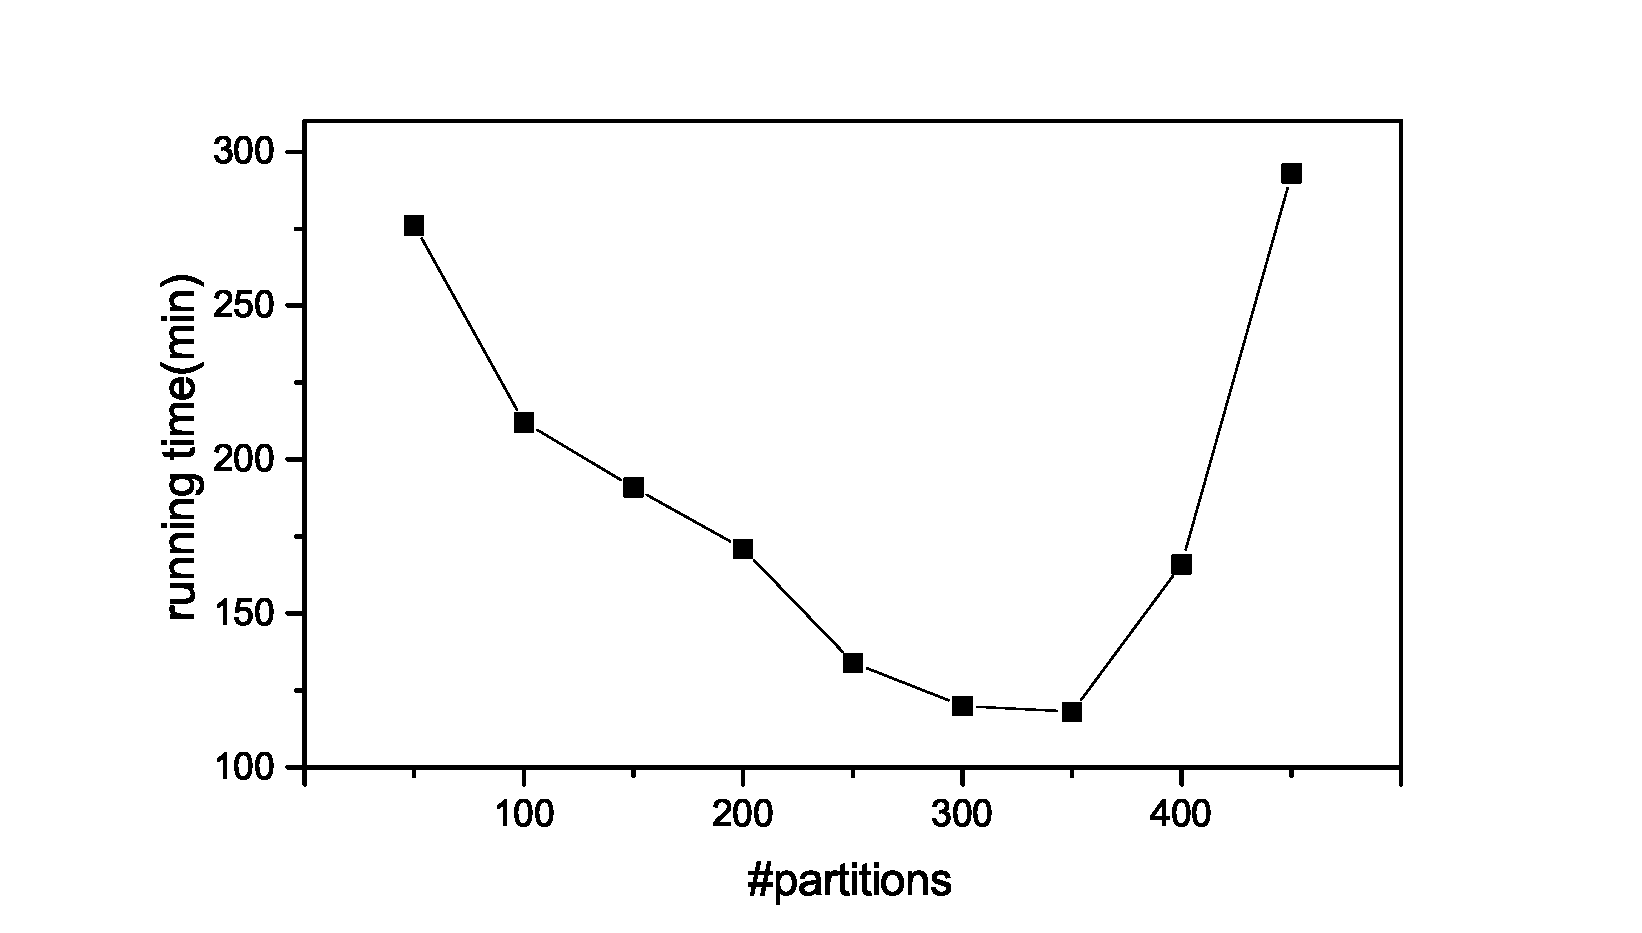
\includegraphics[width= 0.75\textwidth]{figure/ch3_partition_time.eps}\\
  \caption{arabic-2005数据分块数目与运行时间的关系}
  \label{fig:ch3_partition_time}
\end{figure}

图\ref{fig:ch3_partition_time}考察预处理得到的分块数目与算法总体运行时间的关系,这里的时间也包括了图划分的运行时间。
算法的输入数据是三个图中规模最大的图arabic-2005,SimRank计算的迭代次数设置为$k=6$,
运行时使用集群全部的计算节点,其它参数固定不变,只变化分块数$\alpha$的值。
从图中可以看出,运行时间曲线表现为明显的凸性。
分块数目较少意味着图划分算法迭代次数较多,因为只有充分迭代划分算法才可以得到充分少的分块的数量。
当分块数目逐渐增大时,划分算法的迭代次数也随之减少,但此时计算每个分块的块内SimRank相似度代价很高,
因为我们的集群总共大约只有144个核心可以利用,这是并行度的上限。更多的计算任务使得有限的CPU资源成为瓶颈。
从图中还可以看出,分块数目的最优设置大约在300-350左右。
\subsection{算法的可扩展性}
\begin{figure}[h]
\centering
\begin{subfigure}[b]{0.48\textwidth}
	\center
	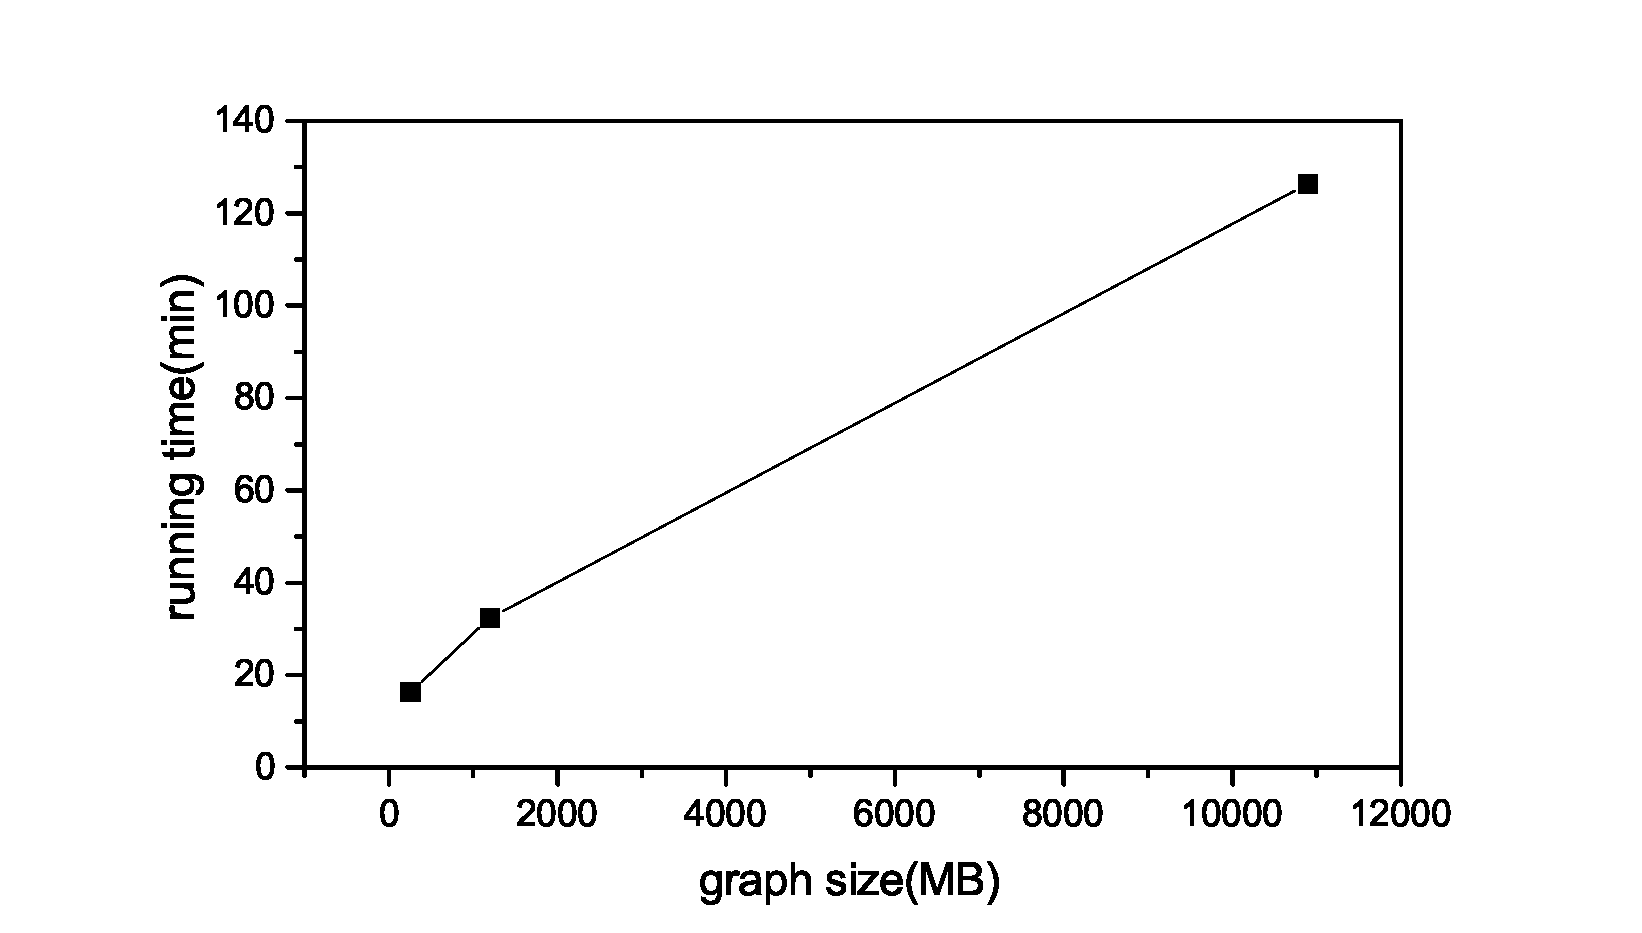
\includegraphics[width=1\textwidth]{figure/ch3_data_scalabity.eps}
	\caption{运行时间与输入图大小的变化关系}
	\label{fig:ch3:data_scalabity}
\end{subfigure}
\begin{subfigure}[b]{0.48\textwidth}
	\centering
	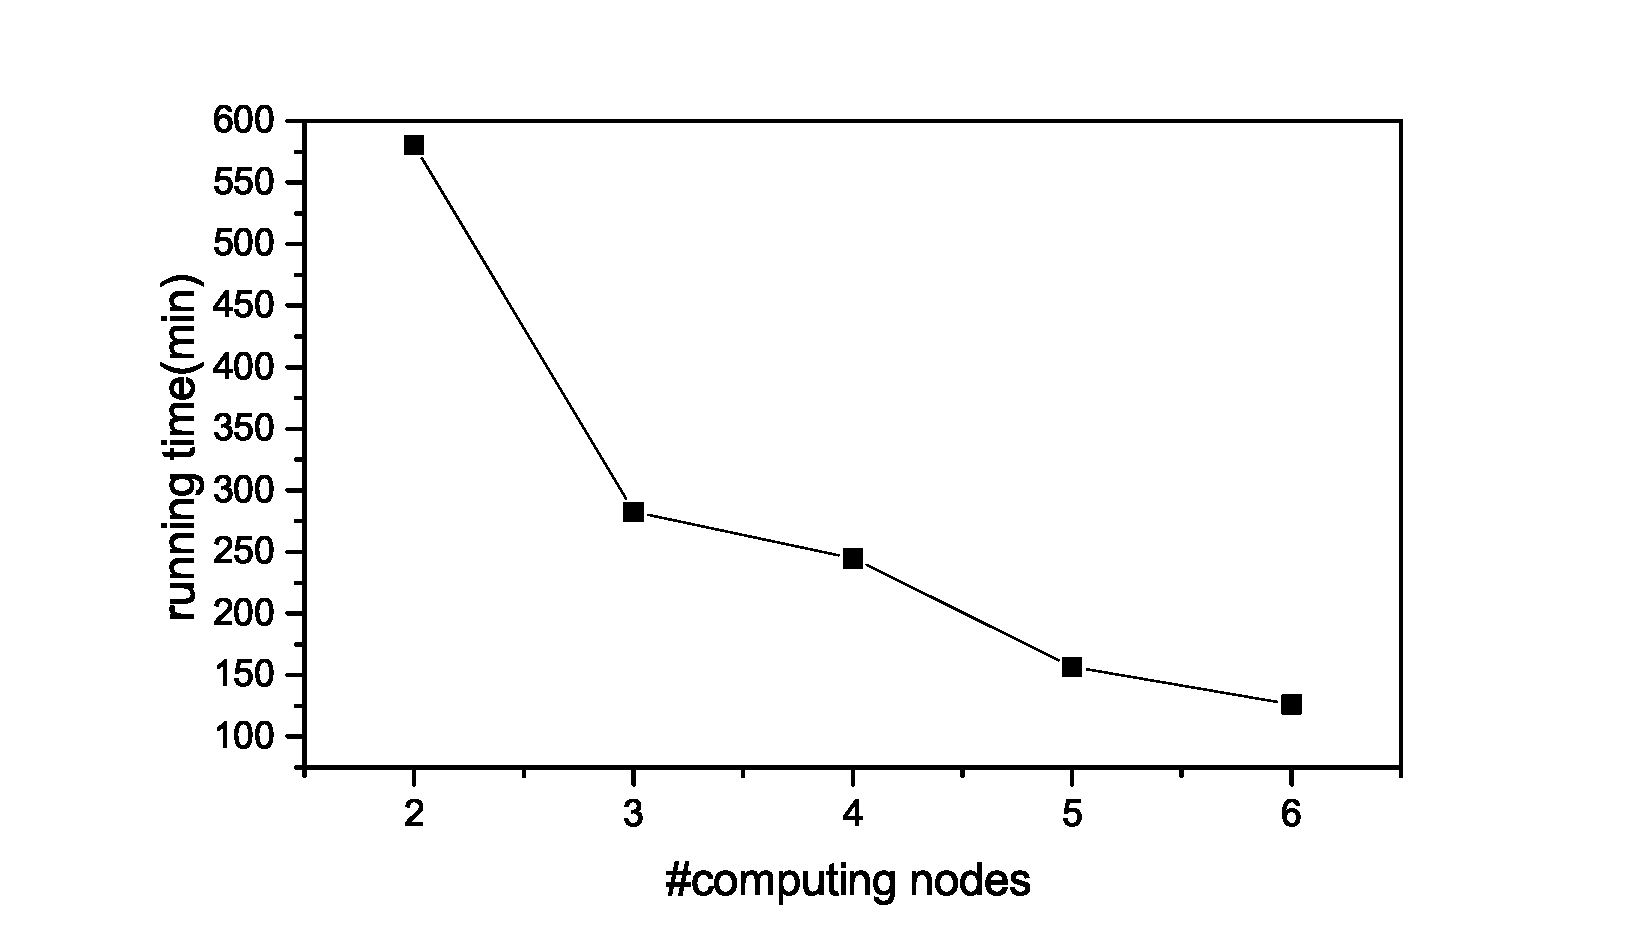
\includegraphics[width=1\textwidth]{figure/ch3_node_scalability.eps}
	\caption{运行时间与计算节点数量的变化关系}
	\label{fig:ch3:node_scalabity}
\end{subfigure}
\caption{算法的可扩展性}
\label{fig:ch3:scala}
\end{figure}
图\ref{fig:ch3:scala}展示了算法的可扩展性。
首先考察算法运行时间随着输入图的大小的变化关系,结果如图\ref{fig:ch3:data_scalabity}所示。
图中展示了当集群计算节点数目固定时,对于不同的图数据,运行时间随输入图规模大小变化的情况。 
算法运行时,设置参数分块数$\alpha=300$,SimRank迭代次数$k=6$,其它参数固定不变。
可以看出,输入图的规模从256MB增长到10.9GB,而对应的运行时间基本上近似的随着输入规模大小线性地变化,
这表明mod\string_MLP具有良好的数据可扩展性。
我们还考察了当输入图的规模固定时,算法运行效率随集群中计算节点数量变化的情况。
输入图为三个图中规模最大的图arabic-2005,运行时固定所有参数,计算节点数量从2增加到6。
实验结果如图\ref{fig:ch3:node_scalabity}所示。
从图中可以看到,对不同规模的输入图,算法的运行时间随集群计算节点的增加而近乎线性地减少,
这表明算法在分布式环境下具有良好的节点可扩展性。

\section{本章小结}
前面章节叙述了计算单源点相似度的计算问题,本章更进一步,把对大规模图数据中的点对SimRank相似度计算推进到全点对问题。
然而考对于现实生活中的拥有数百万节点的大规模图数据,其邻接矩阵的元素规模达到万亿级别($|V|^2$ ),
现有的方法无法对其进行有效计算。

为了能够有效降低问题的复杂度,本章基于图中稠密的分块往往蕴含了最多的人们感兴趣的信息这一事实,
提出一基于种分而治之思想的算法,将点对全局的相似度从两个层次上进行分解:
所属分块间的相似度以及分块内点对的相似度。
然后通过这两个相似度计算任意点对的全局相似度。
实验证明本算法具有高有效性和良好的可并行度。
%%%%%%%%%%%%%%%%%%%%%%%%%%%%%%%%%%%%%%%%%%%%%%%%%%%%%%%%%%%%%%%%%%%%%%%%%%%%%%%
% 学位论文的正文应以《结论》作为最后一章
\chapter{总结与展望}\label{chapter_concludes}
\section{全文工作总结}
图作为能够刻画事物之间联系的通用数据结构,在现实生活中无处不在。
而图中顶点的相似度衡量在众多领域有大量的运用。
本文关注SimRank相似度的计算。
相比于其它度量它能够更好地反映图的拓扑结构,因此成为近年来比较流行的相似度指标。
但是SimRank的计算复杂度较高,而在目前的大数据时代,图数据的规模急剧增长,传统的单机计算方法已经远远不能处理大规模图数据中的点对相似度计算。
另一方面,伴随着Hadoop、Spark等通用分布式计算引擎的流行,分布式计算成为当下的潮流。

在这样的背景下,本文着重研究设计并实现了基于Spark平台的分布式SimRank相似度计算方法,取得的主要成果如下:
\begin{enumerate}
 \item 针对单源点SimRank相似度的计算问题,即给定一个查询节点$u$,计算它与图中其它所有点对的相似度,提出并实现了一种基于随机游走模型的分布式计算方法。
 本文还充分优化了算法中的关键步骤。该算法具有效率高、并行度好的特点。
 \item 为了能够将图进行划分以方便后续处理,本文提出了一种基于模块度优化的大规模图数据的分布式划分方法。 该算法能够较好地保留图中的稠密子图,
 并且划分结果做到了顶点分配均衡。实验结果表明算法具有极好的划分质量,同时拥有较高的执行效率和良好的可扩展性。
 \item 基于上述图划分结果,提出了一种基于分而治之思想的全点对相似度计算方法。 算法将相似性分为两个层次:分块之间的相似性,以及同一分块内点对的相似性。
 任意点对的全局相似度通过它们计算得出。 算法在实际数据集上表现出了高有效性,并且极大地降低了计算时间。
\end{enumerate}

\section{下一步工作展望}
本文提出的算法已经在真实数据集上证明了其优越性,但仍存在一定的不足,还需要进一步研究,这主要体现在以下几个方面:
\begin{enumerate}
 \item 本文提出的图划分算法只考虑了最终划分结果的顶点数量的分配均衡,并没有考虑每个分块内边的数量的相对均衡。
 由于边的数量往往超过顶点的数量,因此对于一些结构特殊的图,这样的策略无法得到最佳的划分结果。
 \item 由于本文单源点、全点对的相似度算法都基于Spark实现,出于对平台的一致性考虑本文提出的分布式图划分算法也基于构建于Spark之上的库GraphX。
 然而,全点对相似度算法要求我们的图划分算法以顶点为基本划分单位,但GraphX底层实现机制中图是按边划分的。这两者的差异虽然不会对最终划分质量造成影响,
 但有可能一定程度上降低了算法的运行效率。
 \item 本文提出的计算全点对复杂度的分布式计算方法计算的是近似的SimRank,虽然其有效性在真实数据集上得到了验证,
 但是我们的近似过程比较粗糙,并没有严密理论来源。 对于一些结构特殊的图,我们提出的计算方式可能会与实际SimRank数值存在偏差。
 
\end{enumerate}



%%%%%%%%%%%%%%%%%%%%%%%%%%%%%%%%%%%%%%%%%%%%%%%%%%%%%%%%%%%%%%%%%%%%%%%%%%%%%%%
% 致谢,应放在《结论》之后
\begin{acknowledgement}
白驹过隙间,我的三年硕士研究生生涯就要结束,我在南京大学七年的学习生活就要划上句号。
即将离别校园之际,回想三年的校园生活,很多情景都历历在目。
研究生阶段,我的科研能力得到了提升,生活上也变得更加独立。
在这里我衷心感谢我的导师、师兄弟、同学、朋友们,你们平时对我的教导、支持、帮助让我愉快地走完了这不平凡的三年,感谢你们!

首先感谢我的导师唐杰。唐老师为人谦和,工作负责,在学术上对我们尽心尽力地指导,在生活上对我们也多有照顾。
无论是本课题的研究及论文的撰写,还是平时对我科研能力的塑造,唐老师都以身作则,对我提供了很多帮助。
唐老师宽厚谦和的生活作风也潜移默化地影响着我,指导着我做一个脚踏实地的南大人。

我还要感谢武港山老师。武老师是多媒体教研室主任,他作风严瑾,要求严格,把握着最新的科研动向,同时管理着整个大组的研究学习工作。
在此特别感谢武老师对我学习和生活上提供的种种帮助。

还要感谢实验室的师兄师弟以及师妹们。三年以来你们给了我很多的关心和支持,很高兴能和你们同门,你们让我留下了很多美好的回忆。
祝愿两位老师身体健康,万事如意! 也祝各位同学学业有成,科研顺利!
最后感谢我的家人,他们永远是我最大的支柱和依靠!

\end{acknowledgement}

% 推荐使用BibTeX,若不使用BibTeX时注释掉下面一句。
\nocite{*}
\bibliography{sample-master}
% 不使用 BibTeX
%\begin{thebibliography}{2}
%
%\bibitem{deng:01a}
%{邓建松,彭冉冉,陈长松}.
%\newblock {\em \LaTeXe{}科技排版指南}.
%\newblock 科学出版社,书号:7-03-009239-2/TP.1516, 北京, 2001.
%
%\bibitem{wang:00a}
%王磊.
%\newblock {\em \LaTeXe{}插图指南}.
%\newblock 2000.
%\end{thebibliography}

% 附录,必须放在参考文献后,backmatter前
%\appendix


%%%%%%%%%%%%%%%%%%%%%%%%%%%%%%%%%%%%%%%%%%%%%%%%%%%%%%%%%%%%%%%%%%%%%%%%%%%%%%%
% 书籍附件
%\backmatter
%%%%%%%%%%%%%%%%%%%%%%%%%%%%%%%%%%%%%%%%%%%%%%%%%%%%%%%%%%%%%%%%%%%%%%%%%%%%%%%
% 作者简历与科研成果页,应放在backmatter之后
\begin{resume}
% 论文作者身份简介,一句话即可。
\begin{authorinfo}
\noindent 高兴坤,男,汉族,1993年01月出生,江苏省泰州人。
\end{authorinfo}
% 论文作者教育经历列表,按日期从近到远排列,不包括将要申请的学位。
\begin{education}
\item[2015年9月 --- 2018年6月] 南京大学计算机科学与技术系 \hfill 硕士
\item[2011年9月 --- 2015年6月] 南京大学计算机科学与技术系 \hfill 本科
\end{education}
% 论文作者在攻读学位期间所发表的文章的列表,按发表日期从近到远排列。
\begin{publications}
\item Xingkun Gao,Nianyuan Bao,Jie Liu,Jie Tang,Gangshan Wu, 
``Scalable Single-Source SimRank Computation for Large Graphs,'' in \textsl{Proc. 22nd IEEE International
    Conference on Parallel and Distributed Systems (ICPADS) 2016}, Dec. 2016.
\end{publications}
% 论文作者在攻读学位期间参与的科研课题的列表,按照日期从近到远排列。
\iffalse
\begin{projects}
\item 国家自然科学基金面上项目``无线传感器网络在知识获取过程中的若干安全问题研究''
(课题年限~2010年1月 --- 2012年12月),负责位置相关安全问题的研究。
\item 江苏省知识创新工程重要方向项目下属课题``下一代移动通信安全机制研究''
(课题年限~2010年1月 --- 2010年12月),负责LTE/SAE认证相关的安全问题研究。
\end{projects}
\fi
\end{resume}

%%%%%%%%%%%%%%%%%%%%%%%%%%%%%%%%%%%%%%%%%%%%%%%%%%%%%%%%%%%%%%%%%%%%%%%%%%%%%%%
% 生成《学位论文出版授权书》页面,应放在最后一页
%\makelicense

%%%%%%%%%%%%%%%%%%%%%%%%%%%%%%%%%%%%%%%%%%%%%%%%%%%%%%%%%%%%%%%%%%%%%%%%%%%%%%%
\end{document}

